\pdfinfoomitdate=1
\pdftrailerid{}
\pdfsuppressptexinfo=-1
\documentclass[10pt,a4paper]{article}
\usepackage{cmap}
\usepackage[margin=1.8cm,headheight=14pt,headsep=10pt]{geometry}
\usepackage[leqno]{amsmath}
\usepackage{amssymb,booktabs,longtable,array,ragged2e,multicol,multirow,xcolor,fancyhdr,tikz}
\definecolor{linkblue}{rgb}{0.08,0.33,0.58}
\usepackage[colorlinks=true,linkcolor=linkblue,urlcolor=linkblue,citecolor=linkblue,
  filecolor=linkblue,linktoc=all,pdfborder={0 0 0},bookmarksnumbered=true]{hyperref}
\setlength{\parindent}{0pt}\setlength{\parskip}{4pt}
\setcounter{secnumdepth}{2}\setcounter{tocdepth}{2}
\definecolor{partshade}{gray}{0.9}
\definecolor{parttitle}{rgb}{0.6,0.1,0.1}
\definecolor{parttitlelight}{HTML}{EC6B60}
\makeatletter
\renewcommand\section{\@startsection{section}{1}{\z@}{-3ex plus -1ex minus -.2ex}%
  {1.2ex plus .2ex}{\normalfont\large\sffamily\bfseries\color{parttitle}}}
\renewcommand\subsection{\@startsection{subsection}{2}{\z@}{-2.5ex plus -1ex minus -.2ex}%
  {.8ex plus .2ex}{\normalfont\sffamily\bfseries\color{parttitle}}}
\renewcommand\subsubsection{\@startsection{subsubsection}{3}{\z@}{-2ex plus -1ex minus -.2ex}%
  {.6ex plus .2ex}{\normalfont\small\sffamily\bfseries\color{parttitle}}}
\renewcommand\paragraph{\@startsection{paragraph}{4}{\z@}{1.5ex plus .5ex minus .2ex}{-1em}%
  {\normalfont\small\sffamily\bfseries\color{parttitle}}}
\renewcommand\tagform@[1]{\maketag@@@{\textsf{\bfseries\footnotesize (#1)}}}
\renewcommand*\l@part[2]{\par\addvspace{1.6ex}\noindent{\sffamily\bfseries #1}\hfill
  {\sffamily\bfseries #2}\par\nobreak}
\newcommand\tocnumber{1.8em}
\newcommand\tocline[4]{\par{\rightskip \tocnumber plus 1fil\relax\parfillskip -\rightskip
  \noindent\hangindent\dimexpr#1+#2\relax\hspace*{#1}%
  \@tempdima #2{\sffamily\small #3}\nobreak\leaders\hbox{$\m@th\mkern 4.5mu\hbox{.}%
  \mkern 4.5mu$}\hfill\nobreak\hbox to \tocnumber{\hfil\sffamily\small #4}\par}}
\renewcommand*\l@section[2]{\tocline{0em}{2.2em}{#1}{#2}}
\renewcommand*\l@subsection[2]{\tocline{2.2em}{2.6em}{#1}{#2}}
\newcommand\contentspage{{\setlength{\columnsep}{24pt}\begin{multicols}{2}\@starttoc{toc}%
  \end{multicols}}}
\newcounter{docpart}\@addtoreset{section}{docpart}
\renewcommand\thesection{\ifnum\value{docpart}>0 \arabic{docpart}.\fi\arabic{section}}
\renewcommand\theHsection{\arabic{docpart}.\arabic{section}}
\newcommand\partnumber[1]{#1\enspace}
\pdfstringdefDisableCommands{\def\partnumber#1{#1 }}
\newcommand{\partbox}[1]{\par\addvspace{12pt}\refstepcounter{docpart}\phantomsection
  \addcontentsline{toc}{part}{\protect\partnumber{\thedocpart}#1}%
  \noindent\colorbox{partshade}{\makebox[%
  \dimexpr\textwidth-2\fboxsep\relax]{\rule[-6pt]{0pt}{20pt}\Large\sffamily\bfseries%
  \textcolor{parttitle}{\thedocpart\quad #1}}}\par\nobreak\@nobreaktrue\addvspace{2pt}}
\newmarks\LTstartmarks\newcount\LTstartcount
\let\LT@startplain\LT@start
\def\LT@start{\global\advance\LTstartcount\@ne\LT@startplain
  \marks\LTstartmarks{\the\LTstartcount}}
\newmarks\LTgroupmarks
\newcount\LTspacebreak\LTspacebreak=-1
\newcount\LTrulebreak\LTrulebreak=-2
\def\grouprule#1#2{\noalign{\marks\LTgroupmarks{\the\belowrulesep}\nobreak\vskip#1%
  \vskip\aboverulesep}\multispan\LT@cols\unskip{\leaders\hrule\@height#2\hfill\kern\z@}\cr
  \noalign{\penalty\LTrulebreak\vskip\belowrulesep\global\@lastruleclass\z@}}
\def\groupspace#1{\noalign{\marks\LTgroupmarks{\the\dimexpr#1\relax}\penalty\LTspacebreak
  \vskip#1\global\@lastruleclass\z@}}
\def\LT@unskips{\unskip\unpenalty\unskip\unpenalty\unskip\unpenalty\unskip\unpenalty}
\def\LT@groupcut{\ifnum\outputpenalty=\LTrulebreak
  \setbox\@cclv\vbox{\unvbox\@cclv\setbox\z@\lastbox\LT@unskips}\fi}
\def\LT@groupjoin{\ifnum\outputpenalty=\LTspacebreak\vskip-\botmarks\LTgroupmarks\relax\fi
  \ifnum\outputpenalty=\LTrulebreak\vskip-\botmarks\LTgroupmarks\relax\fi}
\let\LT@outputplain\LT@output
\def\LT@output{\ifnum\outputpenalty<-\@Mi\LT@outputplain\else
  \edef\LT@marka{\botmarks\LTstartmarks}\edef\LT@markb{\the\LTstartcount}%
  \ifx\LT@marka\LT@markb\LT@groupcut\LT@outputplain\LT@groupjoin
  \else\setbox\LT@head\box\voidb@x\LT@outputplain\fi\fi}
\makeatother
\newcommand{\needspace}[1]{\par\penalty-100\begingroup\dimen0=#1\relax\dimen2=\pagegoal
  \advance\dimen2-\pagetotal\ifdim\dimen0>\dimen2\relax\ifdim\dimen2>0pt\vfil\break\fi\fi
  \endgroup}
\numberwithin{equation}{section}
\pagestyle{fancy}\fancyhf{}
\renewcommand{\headrulewidth}{0pt}
\renewcommand{\sectionmark}[1]{\markright{\thesection\enspace #1}}
\renewcommand{\subsectionmark}[1]{}
\fancyhead[R]{\small\textsc{\rightmark}\quad\thepage}
\fancypagestyle{plain}{\fancyhf{}\fancyfoot[C]{\small\thepage}}
\definecolor{atlasI}{HTML}{991A1A}\definecolor{atlasIl}{HTML}{EC6B60}
\definecolor{atlasII}{HTML}{295A2C}\definecolor{atlasIIl}{HTML}{6C9F6D}
\definecolor{atlasIII}{HTML}{7A1466}\definecolor{atlasIIIl}{HTML}{D66EBC}
\definecolor{atlasIV}{HTML}{9B690B}\definecolor{atlasIVl}{HTML}{F2A618}
\makeatletter
\newcommand\atlas@full{%
\fill[atlasIII] (0.0394,0.0163) -- (0.3978,0.0163) arc[start angle=0.668, end angle=13.836, radius=1.3979] -- cycle;
\fill[atlasI] (-0.0163,0.0394) -- (-0.0163,0.3978) arc[start angle=90.668, end angle=103.836, radius=1.3979] -- cycle;
\fill[atlasIV] (-0.0394,-0.0163) -- (-0.3978,-0.0163) arc[start angle=-179.332, end angle=-166.164, radius=1.3979] -- cycle;
\fill[atlasII] (0.0163,-0.0394) -- (0.0163,-0.3978) arc[start angle=-89.332, end angle=-76.164, radius=1.3979] -- cycle;
\fill[atlasIIIl] (0.0163,0.0394) -- (0.3343,0.3573) arc[start angle=76.164, end angle=89.332, radius=1.3979] -- cycle;
\fill[atlasIl] (-0.0394,0.0163) -- (-0.3573,0.3343) arc[start angle=166.164, end angle=179.332, radius=1.3979] -- cycle;
\fill[atlasIVl] (-0.0163,-0.0394) -- (-0.3343,-0.3573) arc[start angle=-103.836, end angle=-90.668, radius=1.3979] -- cycle;
\fill[atlasIIl] (0.0394,-0.0163) -- (0.3573,-0.3343) arc[start angle=-13.836, end angle=-0.668, radius=1.3979] -- cycle;
\fill[atlasIIIl] (0.4304,0.0163) -- (0.9598,0.0163) arc[start angle=46.637, end angle=73.849, radius=1.3979] arc[start angle=13.862, end angle=0.653, radius=1.4305] -- cycle;
\fill[atlasIl] (-0.0163,0.4304) -- (-0.0163,0.9598) arc[start angle=136.637, end angle=163.849, radius=1.3979] arc[start angle=103.862, end angle=90.653, radius=1.4305] -- cycle;
\fill[atlasIVl] (-0.4304,-0.0163) -- (-0.9598,-0.0163) arc[start angle=-133.363, end angle=-106.151, radius=1.3979] arc[start angle=-166.138, end angle=-179.347, radius=1.4305] -- cycle;
\fill[atlasIIl] (0.0163,-0.4304) -- (0.0163,-0.9598) arc[start angle=-43.363, end angle=-16.151, radius=1.3979] arc[start angle=-76.138, end angle=-89.347, radius=1.4305] -- cycle;
\fill[atlasIII] (0.0163,0.4304) arc[start angle=89.347, end angle=76.138, radius=1.4305] arc[start angle=16.151, end angle=43.363, radius=1.3979] -- cycle;
\fill[atlasI] (-0.4304,0.0163) arc[start angle=179.347, end angle=166.138, radius=1.4305] arc[start angle=106.151, end angle=133.363, radius=1.3979] -- cycle;
\fill[atlasIV] (-0.0163,-0.4304) arc[start angle=-90.653, end angle=-103.862, radius=1.4305] arc[start angle=-163.849, end angle=-136.637, radius=1.3979] -- cycle;
\fill[atlasII] (0.4304,-0.0163) arc[start angle=-0.653, end angle=-13.862, radius=1.4305] arc[start angle=-73.849, end angle=-46.637, radius=1.3979] -- cycle;
\fill[atlasIII] (0.9997,0.0232) arc[start angle=1.329, end angle=44.066, radius=1] -- (0.3973,0.3742) arc[start angle=73.875, end angle=45.664, radius=1.4305] -- cycle;
\fill[atlasI] (-0.0232,0.9997) arc[start angle=91.329, end angle=134.066, radius=1] -- (-0.3742,0.3973) arc[start angle=163.875, end angle=135.664, radius=1.4305] -- cycle;
\fill[atlasIV] (-0.9997,-0.0232) arc[start angle=-178.671, end angle=-135.934, radius=1] -- (-0.3973,-0.3742) arc[start angle=-106.125, end angle=-134.336, radius=1.4305] -- cycle;
\fill[atlasII] (0.0232,-0.9997) arc[start angle=-88.671, end angle=-45.934, radius=1] -- (0.3742,-0.3973) arc[start angle=-16.125, end angle=-44.336, radius=1.4305] -- cycle;
\fill[atlasIIIl] (0.0232,0.9997) arc[start angle=44.336, end angle=16.125, radius=1.4305] -- (0.6955,0.7185) arc[start angle=45.934, end angle=88.671, radius=1] -- cycle;
\fill[atlasIl] (-0.9997,0.0232) arc[start angle=134.336, end angle=106.125, radius=1.4305] -- (-0.7185,0.6955) arc[start angle=135.934, end angle=178.671, radius=1] -- cycle;
\fill[atlasIVl] (-0.0232,-0.9997) arc[start angle=-135.664, end angle=-163.875, radius=1.4305] -- (-0.6955,-0.7185) arc[start angle=-134.066, end angle=-91.329, radius=1] -- cycle;
\fill[atlasIIl] (0.9997,-0.0232) arc[start angle=-45.664, end angle=-73.875, radius=1.4305] -- (0.7185,-0.6955) arc[start angle=-44.066, end angle=-1.329, radius=1] -- cycle;
}
\newcommand\atlas@draw[2]{\begin{tikzpicture}[x=\dimexpr(#1)/2\relax,y=\dimexpr(#1)/2\relax]
\useasboundingbox (-1,-1) rectangle (1,1);#2\end{tikzpicture}}
\newcommand\atlas@volume[1]{{%
\colorlet{atlasI}{parttitle}\colorlet{atlasIl}{parttitlelight}%
\colorlet{atlasII}{parttitle}\colorlet{atlasIIl}{parttitlelight}%
\colorlet{atlasIII}{parttitle}\colorlet{atlasIIIl}{parttitlelight}%
\colorlet{atlasIV}{parttitle}\colorlet{atlasIVl}{parttitlelight}%
#1}}
\newcommand\atlasmark[1]{\atlas@draw{#1}{\atlas@full}}
\newcommand\volumemark[1]{\atlas@volume{\atlasmark{#1}}}
\makeatother
\fancypagestyle{opening}{\fancyhf{}\fancyfoot[C]{\small\thepage}%
  \fancyhead[L]{\smash{\raisebox{-9.5mm}{\volumemark{12mm}}}}}
\hypersetup{pdftitle={Dinfh: Point Group Atlas, volume I: point groups}, pdfauthor={Victor V. Albert}, pdfsubject={Point Group Atlas record Dinfh, schema point-group-atlas/group-continuous/1}}
\fancyhead[L]{\small $\grp{D_{\infty h}}$}
\DeclareMathAlphabet{\mathelt}{OT1}{cmss}{m}{sl}
\DeclareSymbolFont{eltgreek}{OML}{cmssm}{m}{it}
\DeclareMathSymbol{\eltsigma}{\mathord}{eltgreek}{"1B}
\DeclareSymbolFont{eltletters}{OT1}{cmss}{m}{sl}
\DeclareMathSymbol{g}{\mathalpha}{eltletters}{`g}
\DeclareMathSymbol{h}{\mathalpha}{eltletters}{`h}
\DeclareMathSymbol{Q}{\mathalpha}{eltletters}{`Q}
\DeclareMathSymbol{R}{\mathalpha}{eltletters}{`R}
\DeclareMathSymbol{\xi}{\mathord}{eltgreek}{"18}
\newcommand{\eltfont}[1]{{\let\sigma\eltsigma\mathelt{#1}}}
\newcommand{\grp}[1]{\mathsf{#1}}
\newcommand{\irr}[1]{\text{\normalfont\scshape #1}}
\newcommand{\conjpair}[1]{{}^{#1}}
\newcommand{\detbox}[1]{{\setlength{\fboxsep}{1pt}\fbox{#1}}}
\newcommand{\cls}[1]{\eltfont{#1}}
\newcommand{\comp}[1]{\eltfont{#1}}
\newcommand{\elt}[1]{\eltfont{#1}}
\newcommand{\hmname}[1]{#1}
\newcommand{\orbname}[1]{#1}
\newcommand{\conwayname}[1]{#1}
\newcommand{\igname}[1]{#1}
\newcommand{\olivename}[1]{#1}
\newcommand{\spec}[1]{\mathrm{#1}}
\newcommand{\ptag}[1]{\mathrm{#1}}
\newcommand{\orbital}[1]{\mathrm{#1}}
\newcommand{\dirprod}{\times}
\newcommand{\sdprod}{\rtimes}
\newcommand{\samecls}{\cong}
\newcommand{\nconj}[1]{{\scriptsize$\times#1$}}
\newcommand{\clsletter}[1]{\,{\scriptsize\color{black!55}#1}}
\newcommand{\metclasses}[1]{\,{\scriptsize$\{#1\}$}}
\newcommand{\Cyc}[1]{\grp{Z_{#1}}}
\newcommand{\Dih}[1]{\grp{Dih_{#1}}}
\newcommand{\Alt}[1]{\grp{Alt_{#1}}}
\newcommand{\Sym}[1]{\grp{Sym_{#1}}}
\newcommand{\dirvec}[3]{(#1, #2, #3)}
\newcommand{\grpindex}[2]{[#1 : #2]}
\newcommand{\iverson}[1]{[#1]}
\newcommand{\restr}[2]{#1\!\downarrow#2}
\newcommand{\Ind}[2]{\operatorname{Ind}_{#1}^{#2}}
\newcommand{\genidx}[2]{#1^{[\mathrm{#2}]}}
\newcommand{\pointr}{\mathbf{r}}
\newcommand{\unitaxis}{\hat{\mathbf{v}}}
\newcommand{\vv}{\mathbf{v}}
\newcommand{\iunit}{\mathrm{i}}
\newcommand{\expe}{\mathrm{e}}
\newcommand{\diff}{\mathrm{d}}
\newcommand{\goldenratio}{\varphi}
\newcommand{\rootunity}[1]{\zeta_{#1}}
\newcommand{\irrJ}[1]{D^{(#1)}}
\newcommand{\irrJp}[2]{D^{(#1,#2)}}
\newcommand{\repD}[1]{D^{#1}}
\newcommand{\wignerD}[1]{D^{#1}}
\newcommand{\wignerd}[1]{d^{#1}}
\newcommand{\irchar}[1]{\chi_{#1}}
\newcommand{\chiA}{\chi_{\grp{A}}}
\newcommand{\fsind}{\nu_{\mathrm{FS}}}
\newcommand{\conj}[1]{{#1}^{*}}
\newcommand{\diag}{\operatorname{diag}}
\newcommand{\trace}{\operatorname{tr}}
\newcommand{\irrprod}{\otimes}
\newcommand{\mult}{\kappa}
\newcommand{\intx}{\mu}
\newcommand{\cgnorm}{\mathcal{N}}
\newcommand{\period}{L}
\newcommand{\jm}[2]{\bigl\lvert{}^{#1}_{\,#2}\bigr\rangle}
\newcommand{\cgket}[3]{\bigl\lvert{}^{#1}_{\,#2};#3\bigr\rangle}
\newcommand{\irket}[2]{\bigl\lvert{}^{#1}_{\,#2}\bigr\rangle}
\newcommand{\prodket}[2]{\lvert {#1}\,{#2}\rangle}
\newcommand{\ket}[1]{\lvert #1\rangle}
\newcommand{\matel}[5]{\bigl\langle{}^{#1}_{\,#2}\bigm\vert #3\bigm\vert{}^{#4}_{\,#5}\bigr\rangle}
\newcommand{\cgc}[6]{\bigl\langle{}^{#1}_{\,#2}\,{}^{#3}_{\,#4}\bigm\vert{}^{#5}_{\,#6}\bigr\rangle}
\newcommand{\cgcp}[9]{\bigl\langle{}^{#1,#3}_{\,#2}\,{}^{#4,#6}_{\,#5}\bigm\vert{}^{#7,#9}_{\,#8}\bigr\rangle}
\newcommand{\cgck}[7]{\bigl\langle{}^{#1}_{\,#2}\,{}^{#3}_{\,#4}\bigm\vert{}^{#5}_{\,#6};#7\bigr\rangle}
\newcommand{\cgcone}[3]{\langle #1\,#2\mid #3\rangle}
\newcommand{\irrangle}{\text{--}}
\newcommand{\jahn}[1]{\mathrm{#1}}
\newcommand{\vol}{\operatorname{vol}}
\newcommand{\rodrigues}{\boldsymbol{\rho}}
\newcommand{\fcell}{\mathcal{D}}
\newcommand{\fdomain}{\mathcal{F}}
\newcommand{\lensspace}[2]{\mathsf{L}(#1, #2)}
\newcommand{\twosphere}{\mathsf{S}^{2}}
\newcommand{\projplane}{\mathbb{R}\mathsf{P}^{2}}
\newcommand{\schur}[1]{\mathbb{S}_{#1}}
\newcommand{\shape}[1]{[#1]}
\newcommand{\term}[2]{{}^{#1}#2}
\newcommand{\occ}[1]{\lvert #1\rangle}
\newcommand{\sdet}[1]{\lvert #1\rvert}
\newcommand{\hairsp}{\mkern1mu}
\newenvironment{romanlist}{\begin{enumerate}%
\renewcommand{\labelenumi}{(\roman{enumi})}}%
  {\end{enumerate}}
\makeatletter
\newenvironment{irmatrix}[1]{\null\,\vcenter\bgroup\Let@\restore@math@cr\default@tag
  \baselineskip8\ex@ \lineskip3\ex@ \lineskiplimit\lineskip
  \ialign\bgroup\hfil$\m@th\scriptstyle##$\hfil&&\hskip#1\hfil$\m@th\scriptstyle##$\hfil\crcr}%
  {\crcr\egroup\egroup\,}
\makeatother
\newlength{\fillwidth}\newlength{\cellwidth}\newlength{\colwidth}
\newcommand{\cellmax}[1]{\settowidth{\cellwidth}{#1}%
  \ifdim\cellwidth>\colwidth\setlength{\colwidth}{\cellwidth}\fi}
\newcommand{\fillcap}{\ifdim\colwidth<\fillwidth\setlength{\fillwidth}{\colwidth}\fi}
\newcommand{\signbreak}{\penalty100\relax}
\begin{document}
\thispagestyle{opening}
\begin{center}
{\LARGE\sffamily\bfseries\color{parttitle}The $\grp{D_{\infty h}}$ subgroup of $\grp{O(3)}$}
\end{center}
\contentspage
\needspace{194pt}
\partbox{The group}
\section{Names and structure}\label{s:identification}
Conventions: \href{../../CONVENTIONS.pdf}{CONVENTIONS.pdf}, sections \href{../../CONVENTIONS.pdf\#conv.0.1}{0.1}, \href{../../CONVENTIONS.pdf\#conv.2}{2}, \href{../../CONVENTIONS.pdf\#conv.3}{3} and \href{../../CONVENTIONS.pdf\#conv.12}{12}.
\label{n:index.family.N}\label{n:mark.conjugates}\label{n:mark.classes}{\small\setlength{\fillwidth}{\textwidth}\addtolength{\fillwidth}{-2\tabcolsep}\setlength{\colwidth}{0pt}\cellmax{\texttt{commutator\symbol{95}subgroup}}\cellmax{\texttt{contains\symbol{95}inversion}}\cellmax{\texttt{rotation\symbol{95}subgroup}}\cellmax{\texttt{contains\symbol{95}sigma\symbol{95}h}}\cellmax{\texttt{crystallographic}}\cellmax{\texttt{ihrig\symbol{95}golubitsky}}\cellmax{\texttt{hermann\symbol{95}mauguin}}\cellmax{\texttt{principal\symbol{95}axis}}\cellmax{\texttt{abstract\symbol{95}type}}\cellmax{\texttt{product\symbol{95}form}}\cellmax{\texttt{centralizer}}\cellmax{\texttt{schoenflies}}\cellmax{\texttt{laue\symbol{95}class}}\cellmax{\texttt{normalizer}}\cellmax{\texttt{altmann\symbol{95}T}}\cellmax{\texttt{limit\symbol{95}of}}\cellmax{\texttt{center}}\cellmax{\texttt{olive}}\cellmax{\texttt{polar}}\cellmax{\texttt{type}}\addtolength{\fillwidth}{-\colwidth}\setlength{\colwidth}{0pt}\cellmax{semidirect: $\grp{C_{\infty h}}$${}\sdprod{}$$\grp{C_{s}}$\metclasses{\cls{E}, \comp{\infty\sigma_v}}\,\nconj{\infty}; $\grp{C_{\infty h}}$${}\sdprod{}$$\grp{C_{2}}$\metclasses{\cls{E}, \comp{\infty C_2'}}\,\nconj{\infty}; $\grp{C_{\infty v}}$${}\sdprod{}$$\grp{C_{2}}$\metclasses{\cls{E}, \comp{\infty C_2'}}\,\nconj{\infty}; $\grp{D_{\infty}}$${}\sdprod{}$$\grp{C_{s}}$\metclasses{\cls{E}, \comp{\infty\sigma_v}}\,\nconj{\infty}; $\grp{C_{\infty}}$${}\sdprod{}$$\grp{C_{2h}}$\metclasses{\cls{E}, \comp{\infty C_2'}, \cls{i}, \comp{\infty\sigma_v}}\,\nconj{\infty}; $\grp{C_{\infty}}$${}\sdprod{}$$\grp{C_{2v}}$\metclasses{\cls{E}, \comp{\infty C_2'}, \cls{\sigma_h}, \comp{\infty\sigma_v}}\,\nconj{\infty}}\cellmax{direct: $\grp{C_{\infty v}}$${}\dirprod{}$$\grp{C_{s}}$\metclasses{\cls{E}, \cls{\sigma_h}}; $\grp{C_{\infty v}}$${}\dirprod{}$$\grp{C_{i}}$\metclasses{\cls{E}, \cls{i}}; $\grp{D_{\infty}}$${}\dirprod{}$$\grp{C_{s}}$\metclasses{\cls{E}, \cls{\sigma_h}}; $\grp{D_{\infty}}$${}\dirprod{}$$\grp{C_{i}}$\metclasses{\cls{E}, \cls{i}}}\cellmax{$\grp{D_{\infty h}}$, index 1}\cellmax{$\grp{C_{\infty}}$, index 4}\cellmax{$\grp{D_{\infty}}$, index 2}\cellmax{$\igname{\grp{O(2)} \oplus \grp{Z_{2}^{c}}}$}\cellmax{$\olivename{\grp{O(2)} + \grp{Z_{2}^{c}}}$}\cellmax{$\grp{O(2)}\dirprod\Cyc{2}$}\cellmax{$\grp{D_{\mathnormal{N}h}}$, $N\to\infty$}\cellmax{$\dirvec{0}{0}{1}$}\cellmax{$\grp{C_{2h}}$}\cellmax{$\grp{D_{\infty h}}$}\cellmax{$\hmname{\infty /mm}$}\cellmax{yes}\cellmax{40}\cellmax{II}\cellmax{no}\fillcap\begin{longtable}{@{}l>{\RaggedRight\arraybackslash}p{\fillwidth}@{}}\toprule
\texttt{type} & II\\
\texttt{limit\symbol{95}of} & $\grp{D_{\mathnormal{N}h}}$, $N\to\infty$\\
\grouprule{0pt}{\lightrulewidth}
\texttt{abstract\symbol{95}type} & $\grp{O(2)}\dirprod\Cyc{2}$\\
\grouprule{0pt}{\lightrulewidth}
\texttt{principal\symbol{95}axis} & $\dirvec{0}{0}{1}$\\
\texttt{contains\symbol{95}inversion} & yes\\
\texttt{contains\symbol{95}sigma\symbol{95}h} & yes\\
\texttt{polar} & no\\
\texttt{crystallographic} & no\\
\grouprule{0pt}{\lightrulewidth}
\texttt{laue\symbol{95}class} & \href{Dinfh.pdf}{$\grp{D_{\infty h}}$}, index 1\\
\grouprule{0pt}{\lightrulewidth}
\texttt{rotation\symbol{95}subgroup} & \href{Dinf.pdf}{$\grp{D_{\infty}}$}, index 2\\
\texttt{center} & \href{C2h.pdf}{$\grp{C_{2h}}$}\\
\texttt{commutator\symbol{95}subgroup} & \href{Cinf.pdf}{$\grp{C_{\infty}}$}, index 4\\
\texttt{normalizer} & \href{Dinfh.pdf}{$\grp{D_{\infty h}}$}, index 1\\
\texttt{centralizer} & \href{C2h.pdf}{$\grp{C_{2h}}$}\\
\texttt{product\symbol{95}form} & direct: \href{Cinfv.pdf}{$\grp{C_{\infty v}}$}${}\dirprod{}$\href{C1v.pdf}{$\grp{C_{s}}$}\metclasses{\cls{E}, \cls{\sigma_h}}; \href{Cinfv.pdf}{$\grp{C_{\infty v}}$}${}\dirprod{}$\href{S2.pdf}{$\grp{C_{i}}$}\metclasses{\cls{E}, \cls{i}}; \href{Dinf.pdf}{$\grp{D_{\infty}}$}${}\dirprod{}$\href{C1v.pdf}{$\grp{C_{s}}$}\metclasses{\cls{E}, \cls{\sigma_h}}; \href{Dinf.pdf}{$\grp{D_{\infty}}$}${}\dirprod{}$\href{S2.pdf}{$\grp{C_{i}}$}\metclasses{\cls{E}, \cls{i}}\newline semidirect: \href{Cinfh.pdf}{$\grp{C_{\infty h}}$}${}\sdprod{}$\href{C1v.pdf}{$\grp{C_{s}}$}\metclasses{\cls{E}, \comp{\infty\sigma_v}}\,\nconj{\infty}; \href{Cinfh.pdf}{$\grp{C_{\infty h}}$}${}\sdprod{}$\href{C2.pdf}{$\grp{C_{2}}$}\metclasses{\cls{E}, \comp{\infty C_2'}}\,\nconj{\infty}; \href{Cinfv.pdf}{$\grp{C_{\infty v}}$}${}\sdprod{}$\href{C2.pdf}{$\grp{C_{2}}$}\metclasses{\cls{E}, \comp{\infty C_2'}}\,\nconj{\infty}; \href{Dinf.pdf}{$\grp{D_{\infty}}$}${}\sdprod{}$\href{C1v.pdf}{$\grp{C_{s}}$}\metclasses{\cls{E}, \comp{\infty\sigma_v}}\,\nconj{\infty}; \href{Cinf.pdf}{$\grp{C_{\infty}}$}${}\sdprod{}$\href{C2h.pdf}{$\grp{C_{2h}}$}\metclasses{\cls{E}, \comp{\infty C_2'}, \cls{i}, \comp{\infty\sigma_v}}\,\nconj{\infty}; \href{Cinf.pdf}{$\grp{C_{\infty}}$}${}\sdprod{}$\href{C2v.pdf}{$\grp{C_{2v}}$}\metclasses{\cls{E}, \comp{\infty C_2'}, \cls{\sigma_h}, \comp{\infty\sigma_v}}\,\nconj{\infty}\\
\grouprule{0pt}{\lightrulewidth}
\texttt{altmann\symbol{95}T} & 40\\
\texttt{hermann\symbol{95}mauguin} & $\hmname{\infty /mm}$\\
\texttt{ihrig\symbol{95}golubitsky} & $\igname{\grp{O(2)} \oplus \grp{Z_{2}^{c}}}$\\
\texttt{olive} & $\olivename{\grp{O(2)} + \grp{Z_{2}^{c}}}$\\
\texttt{schoenflies} & \href{Dinfh.pdf}{$\grp{D_{\infty h}}$}\\
\bottomrule\end{longtable}}
\leavevmode\label{n:element.inversion}In this table, \texttt{type} is I when every element of $\grp{D_{\infty h}}$ is a rotation, II when $\grp{D_{\infty h}}$ contains the inversion $\elt{i}$ and III otherwise; \texttt{polar} is yes when $\grp{D_{\infty h}}$ fixes a nonzero vector; crystallographers call a group chiral, or enantiomorphic, when its type is I, and centrosymmetric when it contains $\elt{i}$; \texttt{laue\symbol{95}class} is the group that $\grp{D_{\infty h}}$ and $\elt{i}$ generate.
In \texttt{product\symbol{95}form}, after a semidirect product, ${\times}\infty$ marks infinitely many subgroups conjugate to its second factor; the braces hold the classes of $\grp{D_{\infty h}}$ that the finite second factor meets: atoms of the class space (section~\ref{s:class_space}) and distinguished points of its arcs (\href{../../CONVENTIONS.pdf}{CONVENTIONS.pdf}, section \href{../../CONVENTIONS.pdf\#conv.16}{16}).
\needspace{242pt}
\section{Class space}\label{s:class_space}
Conventions: \href{../../CONVENTIONS.pdf}{CONVENTIONS.pdf}, section \href{../../CONVENTIONS.pdf\#conv.16}{16}.
\leavevmode\label{n:angle.phi}\label{n:mark.atom}\label{n:angle.psi}\label{n:head.component}\label{n:head.coset}\label{n:head.element}A row is a component of the class space, an arc of classes or an atom, a single class; coset tells whether its elements are proper or improper, element gives the element at its angle, and $P$ is the matrix of that element, in the row-vector convention of \href{../../CONVENTIONS.pdf}{CONVENTIONS.pdf}, section \href{../../CONVENTIONS.pdf\#conv.4}{4}; on column vectors it is the transpose $P^{\top}$, and products compose in the reverse order.
\begin{center}\begin{tabular}{@{}llll@{}}\toprule
component & coset & element & $P$\\\midrule
$\comp{C_{\infty}(\phi)}$ & proper & $\elt{C_{\infty}}(\phi)$ & $\left(\begin{smallmatrix}\cos\phi & \sin\phi & 0\\-\sin\phi & \cos\phi & 0\\0 & 0 & 1\end{smallmatrix}\right)$\\
$\comp{\infty C_2'}$ & proper & $\elt{C_2'}(\psi)$ & $\left(\begin{smallmatrix}\cos(2\psi) & \sin(2\psi) & 0\\\sin(2\psi) & -\cos(2\psi) & 0\\0 & 0 & -1\end{smallmatrix}\right)$\\
$\comp{i\,C_{\infty}(\phi)}$ & improper & $\elt{i\,C_{\infty}}(\phi)$ & $\left(\begin{smallmatrix}-\cos\phi & -\sin\phi & 0\\\sin\phi & -\cos\phi & 0\\0 & 0 & -1\end{smallmatrix}\right)$\\
$\comp{\infty\sigma_v}$ & improper & $\elt{\sigma_v}(\psi)$ & $\left(\begin{smallmatrix}\cos(2\psi) & \sin(2\psi) & 0\\\sin(2\psi) & -\cos(2\psi) & 0\\0 & 0 & 1\end{smallmatrix}\right)$\\
\bottomrule\end{tabular}\end{center}
$\comp{\infty C_2'}$ is the class of the binary rotations $\elt{C_2'}(\psi)$ about the horizontal axes at every azimuth $\psi$, $\comp{\infty\sigma_v}$ that of the vertical mirrors $\elt{\sigma_v}(\psi)$.
\leavevmode\label{n:local.haar.h}The Haar measure, of total mass 1, is $\diff h = \diff\phi/(4\pi)$ on $\comp{C_{\infty}(\phi)}$, $\phi\in\bigl[0, \pi\bigr]$, of mass $\tfrac{1}{4}$; $\diff h = \diff\phi/(4\pi)$ on $\comp{i\,C_{\infty}(\phi)}$, $\phi\in\bigl[0, \pi\bigr]$, of mass $\tfrac{1}{4}$; the atoms $\comp{\infty C_2'}$ and $\comp{\infty\sigma_v}$ have mass $\tfrac{1}{4}$ each.
\needspace{103pt}
\section{Fundamental domain}\label{s:fundamental_domain}
Conventions: \href{../../CONVENTIONS.pdf}{CONVENTIONS.pdf}, sections \href{../../CONVENTIONS.pdf\#conv.4.2}{4.2} and \href{../../CONVENTIONS.pdf\#conv.17}{17}.
\leavevmode\label{n:element.placement}\label{n:operator.cosets}A molecule with symmetry $\grp{D_{\infty h}}$ placed by $Q \in \grp{O(3)}$ is the same set of atoms when placed by $gQ$ with $g \in \grp{D_{\infty h}}$, as $P(gQ) = P(g)\,P(Q)$: its orientations are the cosets $\grp{D_{\infty h}}Q = \{gQ : g \in \grp{D_{\infty h}}\}$, the points of the space $\grp{D_{\infty h}}\backslash\grp{O(3)}$. On column vectors the matrices of a coset are $P(Q)^{\top}P(g)^{\top}$, a left coset of the transposes and a point of $\grp{O(3)}/\grp{D_{\infty h}}$.
\leavevmode\label{n:operator.volume}Volumes are those of the invariant metric of \href{O3.pdf}{$\grp{O(3)}$} in which the distance from $\elt{E}$ to a rotation by $\omega \le \pi$ is $\omega$, so that $\vol\grp{SO(3)} = 8\pi^2$ and $\vol\grp{O(3)} = 16\pi^2$; $\grp{D_{\infty h}}$ is the union of the circles $\elt{C_{\infty}}(\phi)$, $\elt{C_2'}(\psi)$, $\elt{i\,C_{\infty}}(\phi)$ and $\elt{\sigma_v}(\psi)$, $\phi \in [0, 2\pi)$ and $\psi \in [0, \pi)$, each of length $2\pi$, so that $\vol\grp{D_{\infty h}} = 8\pi$.

\leavevmode\label{n:angle.euler.alpha}\label{n:angle.euler.beta}\label{n:angle.euler.gamma}$(\alpha,\beta,\gamma)$ are the Euler angles of the rotation $(\det Q)\,Q$: by $\alpha$ about $z$, then by $\beta$ about $y$, then by $\gamma$ about $z$ (fixed axes); the volume element of \href{SO3.pdf}{$\grp{SO(3)}$} is $\sin\beta\,\diff\alpha\,\diff\beta\,\diff\gamma$. As $\elt{C_{\infty}}(\phi)\,Q$ has the angles $(\alpha + \phi, \beta, \gamma)$, a coset of \href{Cinf.pdf}{$\grp{C_{\infty}}$} is a circle of $\alpha$, and $(\beta, \gamma)$ are the polar and azimuthal angles of the axis $\dirvec{0}{0}{1}P((\det Q)\,Q)$ of the molecule: the cosets have the metric of the unit sphere of the axes, of area element $\sin\beta\,\diff\beta\,\diff\gamma$. $\elt{C_2'}(\psi)$ carries the rotation of the angles $(0, \beta, \gamma)$ to that of $(-2\psi, \pi - \beta, \gamma + \pi)$, of the opposite axis.
\leavevmode\label{n:set.cell}The cell $\fcell$ of the rotations with $\alpha = 0$, $\beta \in [0, \tfrac{\pi}{2}]$ and $\gamma \in (-\pi, \pi]$ meets every coset of $\grp{D_{\infty h}} \cap \grp{SO(3)} = \grp{D_{\infty}}$ once, except on its boundary ($\beta = 0$ and $\beta = \tfrac{\pi}{2}$), and, in the metric of the cosets, $\vol\fcell = 2\pi$.

\leavevmode\label{n:set.fundamental}As $\grp{D_{\infty h}}$ holds an improper element, every coset $\grp{D_{\infty h}}Q$ meets \href{SO3.pdf}{$\grp{SO(3)}$} in one coset of $\grp{D_{\infty h}} \cap \grp{SO(3)}$, so that $\fdomain = \fcell$ is a fundamental domain: it holds one element of every coset, more only on its boundary.
\leavevmode\label{n:set.projective}$\grp{D_{\infty h}}\backslash\grp{O(3)}$ is $\grp{D_{\infty}}\backslash\grp{SO(3)}$, the projective plane $\projplane$, and
\begin{equation}\label{e:volume}\vol\fdomain = \vol\fcell = 2\pi,\qquad \vol\grp{D_{\infty h}}\cdot\vol\fdomain = 8\pi\cdot 2\pi = 16\pi^2 = \vol\grp{O(3)}.\end{equation}
\needspace{171pt}
\partbox{Representations}
\section{Families of irreps}\label{s:families}
Conventions: \href{../../CONVENTIONS.pdf}{CONVENTIONS.pdf}, sections \href{../../CONVENTIONS.pdf\#conv.6}{6}, \href{../../CONVENTIONS.pdf\#conv.7}{7} and \href{../../CONVENTIONS.pdf\#conv.16}{16}.
\leavevmode\label{n:irrep.Gamma}\label{n:index.dimension}\label{n:index.frobenius}\label{n:index.family}\label{n:mark.determinant}\label{n:irrep.alias.greek}\label{n:head.family.irreps}\label{n:head.index.family}\label{n:head.aliases}\label{n:head.kernel}\label{n:head.image}A family is a family of irreps, by its label, $d$ the dimension of its irreps and $\fsind$ their Frobenius--Schur indicator (real: $+1$), index the range of the index of its instances, kernel the subgroup $\ker\Gamma$ of the elements that an irrep $\Gamma$ of the family maps to the identity, image the group that its matrices form, isomorphic to $\grp{D_{\infty h}}/\ker\Gamma$, and aliases its other names; a dash stands for none. The image is named by a group of the catalogue: for $d = 1$ the group of the characters, turning the complex plane; for $d = 2$ the group of the matrices in a real basis, in $\grp{O(2)}$ acting on the plane. The irreps are irreducible over $\mathbb{C}$. Each is real, and in a basis with real matrices it is also an irrep over $\mathbb{R}$ (\href{../../CONVENTIONS.pdf}{CONVENTIONS.pdf}, section \href{../../CONVENTIONS.pdf\#conv.7}{7}). The boxed family, of one irrep, is the determinant character (\texttt{determinant\symbol{95}character}), whose character is $\det g$.
{\small\renewcommand{\arraystretch}{1.25}\setlength{\fillwidth}{\textwidth}\addtolength{\fillwidth}{-12\tabcolsep}\setlength{\colwidth}{0pt}\cellmax{family}\cellmax{$\irr{e}_{n,\ptag{g}}$}\cellmax{$\irr{e}_{n,\ptag{u}}$}\cellmax{\detbox{$\irr{a}_{1\ptag{u}}$}}\cellmax{$\irr{a}_{1\ptag{g}}$}\cellmax{$\irr{a}_{2\ptag{g}}$}\cellmax{$\irr{a}_{2\ptag{u}}$}\addtolength{\fillwidth}{-\colwidth}\setlength{\colwidth}{0pt}\cellmax{$d$}\cellmax{1}\cellmax{2}\addtolength{\fillwidth}{-\colwidth}\setlength{\colwidth}{0pt}\cellmax{$\fsind$}\cellmax{$+1$}\addtolength{\fillwidth}{-\colwidth}\setlength{\colwidth}{0pt}\cellmax{index}\cellmax{$n \ge 1$}\cellmax{---}\addtolength{\fillwidth}{-\colwidth}\setlength{\colwidth}{0pt}\cellmax{$\grp{C_{\mathnormal{n}h}}$, $n$ even}\cellmax{$\grp{S_{2\mathnormal{n}}}$, $n$ even}\cellmax{$\grp{C_{\mathnormal{n}h}}$, $n$ odd}\cellmax{$\grp{S_{2\mathnormal{n}}}$, $n$ odd}\cellmax{kernel}\cellmax{$\grp{C_{\infty h}}$}\cellmax{$\grp{C_{\infty v}}$}\cellmax{$\grp{D_{\infty h}}$}\cellmax{$\grp{D_{\infty}}$}\addtolength{\fillwidth}{-\colwidth}\setlength{\colwidth}{0pt}\cellmax{image}\cellmax{$\grp{C_{\infty v}}$}\cellmax{$\grp{C_{1}}$}\cellmax{$\grp{C_{2}}$}\addtolength{\fillwidth}{-\colwidth}\setlength{\colwidth}{0pt}\cellmax{$\Pi_{\ptag{g}}$ ($n = 1$), $\Delta_{\ptag{g}}$ ($n = 2$), $\Phi_{\ptag{g}}$ ($n = 3$)}\cellmax{$\Pi_{\ptag{u}}$ ($n = 1$), $\Delta_{\ptag{u}}$ ($n = 2$), $\Phi_{\ptag{u}}$ ($n = 3$)}\cellmax{aliases}\cellmax{$\Sigma_{\ptag{g}}^{+}$}\cellmax{$\Sigma_{\ptag{g}}^{-}$}\cellmax{$\Sigma_{\ptag{u}}^{+}$}\cellmax{$\Sigma_{\ptag{u}}^{-}$}\fillcap\begin{longtable}{@{}lrrlll>{\RaggedRight\arraybackslash}p{\fillwidth}@{}}\toprule
family & $d$ & $\fsind$ & index & kernel & image & aliases\\\midrule\endhead
\bottomrule\endfoot\endlastfoot
$\irr{a}_{1\ptag{g}}$ & 1 & $+1$ & --- & \href{Dinfh.pdf}{$\grp{D_{\infty h}}$} & \href{C1.pdf}{$\grp{C_{1}}$} & $\Sigma_{\ptag{g}}^{+}$\\*
$\irr{a}_{2\ptag{g}}$ & 1 & $+1$ & --- & \href{Cinfh.pdf}{$\grp{C_{\infty h}}$} & \href{C2.pdf}{$\grp{C_{2}}$} & $\Sigma_{\ptag{g}}^{-}$\\
\multirow{2}{*}{$\irr{e}_{n,\ptag{g}}$} & \multirow{2}{*}{2} & \multirow{2}{*}{$+1$} & \multirow{2}{*}{$n \ge 1$} & $\grp{C_{\mathnormal{n}h}}$, $n$ even & \multirow{2}{*}{\href{Cinfv.pdf}{$\grp{C_{\infty v}}$}} & \multirow{2}{=}{\RaggedRight $\Pi_{\ptag{g}}$ ($n = 1$), $\Delta_{\ptag{g}}$ ($n = 2$), $\Phi_{\ptag{g}}$ ($n = 3$)}\\*
 &  &  &  & $\grp{S_{2\mathnormal{n}}}$, $n$ odd &  & \\
\detbox{$\irr{a}_{1\ptag{u}}$} & 1 & $+1$ & --- & \href{Dinf.pdf}{$\grp{D_{\infty}}$} & \href{C2.pdf}{$\grp{C_{2}}$} & $\Sigma_{\ptag{u}}^{-}$\\
$\irr{a}_{2\ptag{u}}$ & 1 & $+1$ & --- & \href{Cinfv.pdf}{$\grp{C_{\infty v}}$} & \href{C2.pdf}{$\grp{C_{2}}$} & $\Sigma_{\ptag{u}}^{+}$\\
\multirow{2}{*}{$\irr{e}_{n,\ptag{u}}$} & \multirow{2}{*}{2} & \multirow{2}{*}{$+1$} & \multirow{2}{*}{$n \ge 1$} & $\grp{S_{2\mathnormal{n}}}$, $n$ even & \multirow{2}{*}{\href{Cinfv.pdf}{$\grp{C_{\infty v}}$}} & \multirow{2}{=}{\RaggedRight $\Pi_{\ptag{u}}$ ($n = 1$), $\Delta_{\ptag{u}}$ ($n = 2$), $\Phi_{\ptag{u}}$ ($n = 3$)}\\*
 &  &  &  & $\grp{C_{\mathnormal{n}h}}$, $n$ odd &  & \\
\bottomrule\end{longtable}}
\needspace{110pt}
\section{Representation matrices}\label{s:continuous_irreps}
Conventions: \href{../../CONVENTIONS.pdf}{CONVENTIONS.pdf}, sections \href{../../CONVENTIONS.pdf\#conv.9}{9} and \href{../../CONVENTIONS.pdf\#conv.16}{16}.
$\iunit$ is the imaginary unit and $\expe$ the base of the natural logarithm.
\leavevmode\label{n:vector.ket.partner}\label{n:index.partner}\label{n:matrix.irrep}A basis $(\irket{\Gamma}{1}, \dots, \irket{\Gamma}{d})$ of the irrep $\Gamma$ obeys
\begin{equation}\label{e:partner}g\irket{\Gamma}{\intx} = \sum_\nu \irket{\Gamma}{\nu}\, \repD{\Gamma}_{\nu,\intx}(g);\end{equation}
the irreps form families, and a row of a table holds $\repD{\Gamma}(g)$ for the elements of a component of the class space (section~\ref{s:class_space}), as a function of their angle.
\leavevmode\label{n:function.character}The character is the trace, $\irchar{\Gamma}(g) = \trace\repD{\Gamma}(g)$; the record also gives it in closed form on each component (\texttt{character\symbol{95}functions.\allowbreak irrep\symbol{95}families[].\allowbreak chi}).
\needspace{139pt}
\subsection{The irreps of dimension 1}
$\repD{\Gamma}(g) = \irchar{\Gamma}(g)$.
{\small\setlength{\tabcolsep}{4pt}
\begin{longtable}{@{}lllll@{}}\toprule
$g$ & $\irr{a}_{1\ptag{g}}$ & $\irr{a}_{2\ptag{g}}$ & $\irr{a}_{1\ptag{u}}$ & $\irr{a}_{2\ptag{u}}$\\\midrule\endhead
\bottomrule\endfoot\endlastfoot
$\elt{C_{\infty}}(\phi)$ & $1$ & $1$ & $1$ & $1$\\*
$\elt{C_2'}(\psi)$ & $1$ & $-1$ & $1$ & $-1$\\*
$\elt{i\,C_{\infty}}(\phi)$ & $1$ & $1$ & $-1$ & $-1$\\*
$\elt{\sigma_v}(\psi)$ & $1$ & $-1$ & $-1$ & $1$\\
\bottomrule\end{longtable}}
\needspace{168pt}
\subsection{The irreps of dimension 2}\label{s:irreps2}
\leavevmode\label{n:vector.ket.one}\label{n:vector.basis.e}\label{n:index.harmonic}\label{n:index.harmonic.a}\label{n:matrix.real}\label{n:matrix.unitary}\label{n:head.real}In the rotation-diagonal basis $(\ket{e_1}, \ket{e_2}) = \bigl((x-\iunit y)^n z^{\delta}, (x+\iunit y)^n z^{\delta}\bigr)$, $\delta = n \bmod 2$ for $\irr{e}_{n,\ptag{g}}$, $\delta = (n+1) \bmod 2$ for $\irr{e}_{n,\ptag{u}}$, the rotations about $z$ are diagonal; in the real basis $\bigl(\tfrac{1}{2}\sqrt{2}\,(\ket{e_1} + \ket{e_2}), -\tfrac{1}{2}\iunit\sqrt{2}\,(\ket{e_1} - \ket{e_2})\bigr)$ the matrices are $D_{\mathrm{real}} = U D U^\dagger$, $U = \tfrac{1}{2}\sqrt{2}\left(\begin{smallmatrix}1 & 1\\ \iunit & -\iunit\end{smallmatrix}\right)$.
{\small\setlength{\tabcolsep}{4pt}
\begin{longtable}{@{}lll@{}}\toprule
 & \multicolumn{2}{c}{$\repD{\irr{e}_{n,\ptag{g}}}(g)$}\\\cmidrule(lr){2-3}
$g$ & real & rotation-diagonal\\\midrule\endhead
\bottomrule\endfoot\endlastfoot
$\elt{C_{\infty}}(\phi)$ & $\left(\begin{irmatrix}{0.2778em}\cos(n\phi) & -\sin(n\phi)\\\sin(n\phi) & \cos(n\phi)\end{irmatrix}\right)$ & $\left(\begin{irmatrix}{0.2778em}\expe^{-\iunit n\phi} & 0\\0 & \expe^{+\iunit n\phi}\end{irmatrix}\right)$\\*\addlinespace[6pt]
$\elt{C_2'}(\psi)$ & $\left(\begin{irmatrix}{0.2778em}(-1)^n\cos(2n\psi) & -(-1)^n\sin(2n\psi)\\-(-1)^n\sin(2n\psi) & -(-1)^n\cos(2n\psi)\end{irmatrix}\right)$ & $\left(\begin{irmatrix}{0.2778em}0 & (-1)^n\expe^{+\iunit 2n\psi}\\(-1)^n\expe^{-\iunit 2n\psi} & 0\end{irmatrix}\right)$\\\groupspace{6pt}
$\elt{i\,C_{\infty}}(\phi)$ & $\left(\begin{irmatrix}{0.2778em}\cos(n\phi) & -\sin(n\phi)\\\sin(n\phi) & \cos(n\phi)\end{irmatrix}\right)$ & $\left(\begin{irmatrix}{0.2778em}\expe^{-\iunit n\phi} & 0\\0 & \expe^{+\iunit n\phi}\end{irmatrix}\right)$\\*\addlinespace[6pt]
$\elt{\sigma_v}(\psi)$ & $\left(\begin{irmatrix}{0.2778em}\cos(2n\psi) & -\sin(2n\psi)\\-\sin(2n\psi) & -\cos(2n\psi)\end{irmatrix}\right)$ & $\left(\begin{irmatrix}{0.2778em}0 & \expe^{+\iunit 2n\psi}\\\expe^{-\iunit 2n\psi} & 0\end{irmatrix}\right)$\\
\bottomrule\end{longtable}}
{\small\setlength{\tabcolsep}{4pt}
\begin{longtable}{@{}lll@{}}\toprule
 & \multicolumn{2}{c}{$\repD{\irr{e}_{n,\ptag{u}}}(g)$}\\\cmidrule(lr){2-3}
$g$ & real & rotation-diagonal\\\midrule\endhead
\bottomrule\endfoot\endlastfoot
$\elt{C_{\infty}}(\phi)$ & $\left(\begin{irmatrix}{0.2778em}\cos(n\phi) & -\sin(n\phi)\\\sin(n\phi) & \cos(n\phi)\end{irmatrix}\right)$ & $\left(\begin{irmatrix}{0.2778em}\expe^{-\iunit n\phi} & 0\\0 & \expe^{+\iunit n\phi}\end{irmatrix}\right)$\\*\addlinespace[6pt]
$\elt{C_2'}(\psi)$ & $\left(\begin{irmatrix}{0.2778em}-(-1)^n\cos(2n\psi) & (-1)^n\sin(2n\psi)\\(-1)^n\sin(2n\psi) & (-1)^n\cos(2n\psi)\end{irmatrix}\right)$ & $\left(\begin{irmatrix}{0.2778em}0 & -(-1)^n\expe^{+\iunit 2n\psi}\\-(-1)^n\expe^{-\iunit 2n\psi} & 0\end{irmatrix}\right)$\\\groupspace{6pt}
$\elt{i\,C_{\infty}}(\phi)$ & $\left(\begin{irmatrix}{0.2778em}-\cos(n\phi) & \sin(n\phi)\\-\sin(n\phi) & -\cos(n\phi)\end{irmatrix}\right)$ & $\left(\begin{irmatrix}{0.2778em}-\expe^{-\iunit n\phi} & 0\\0 & -\expe^{+\iunit n\phi}\end{irmatrix}\right)$\\*\addlinespace[6pt]
$\elt{\sigma_v}(\psi)$ & $\left(\begin{irmatrix}{0.2778em}\cos(2n\psi) & -\sin(2n\psi)\\-\sin(2n\psi) & -\cos(2n\psi)\end{irmatrix}\right)$ & $\left(\begin{irmatrix}{0.2778em}0 & \expe^{+\iunit 2n\psi}\\\expe^{-\iunit 2n\psi} & 0\end{irmatrix}\right)$\\
\bottomrule\end{longtable}}
\needspace{161pt}
\section{Direct products of irreps}\label{s:fusion}
Conventions: \href{../../CONVENTIONS.pdf}{CONVENTIONS.pdf}, section \href{../../CONVENTIONS.pdf\#conv.10}{10}.
A rule for every pair of families, $n$ and $n'$ their indices; the squares $\Gamma\irrprod\Gamma$ follow, with the antisymmetric part in braces.
\needspace{95pt}
\paragraph{Products.}
{\small\begin{longtable}{@{}l@{${}={}$}ll@{}}\toprule
$\irr{a}_{1\ptag{g}}\irrprod \irr{a}_{1\ptag{g}}$ & $\irr{a}_{1\ptag{g}}$ & \\
$\irr{a}_{1\ptag{g}}\irrprod \irr{a}_{2\ptag{g}}$ & $\irr{a}_{2\ptag{g}}$ & \\
$\irr{a}_{1\ptag{g}}\irrprod \irr{e}_{n,\ptag{g}}$ & $\irr{e}_{n,\ptag{g}}$ & \\
$\irr{a}_{1\ptag{g}}\irrprod \irr{a}_{1\ptag{u}}$ & $\irr{a}_{1\ptag{u}}$ & \\
$\irr{a}_{1\ptag{g}}\irrprod \irr{a}_{2\ptag{u}}$ & $\irr{a}_{2\ptag{u}}$ & \\
$\irr{a}_{1\ptag{g}}\irrprod \irr{e}_{n,\ptag{u}}$ & $\irr{e}_{n,\ptag{u}}$ & \\
$\irr{a}_{2\ptag{g}}\irrprod \irr{a}_{2\ptag{g}}$ & $\irr{a}_{1\ptag{g}}$ & \\
$\irr{a}_{2\ptag{g}}\irrprod \irr{e}_{n,\ptag{g}}$ & $\irr{e}_{n,\ptag{g}}$ & \\
$\irr{a}_{2\ptag{g}}\irrprod \irr{a}_{1\ptag{u}}$ & $\irr{a}_{2\ptag{u}}$ & \\
$\irr{a}_{2\ptag{g}}\irrprod \irr{a}_{2\ptag{u}}$ & $\irr{a}_{1\ptag{u}}$ & \\
$\irr{a}_{2\ptag{g}}\irrprod \irr{e}_{n,\ptag{u}}$ & $\irr{e}_{n,\ptag{u}}$ & \\
$\irr{e}_{n,\ptag{g}}\irrprod \irr{e}_{n',\ptag{g}}$ & $\irr{e}_{n+n',\ptag{g}}\oplus \irr{e}_{\lvert n-n'\rvert,\ptag{g}}$ & $n \ne n'$\\
$\irr{e}_{n,\ptag{g}}\irrprod \irr{e}_{n',\ptag{g}}$ & $\irr{a}_{1\ptag{g}}\oplus \irr{a}_{2\ptag{g}}\oplus \irr{e}_{2n',\ptag{g}}$ & $n = n'$\\
$\irr{e}_{n,\ptag{g}}\irrprod \irr{a}_{1\ptag{u}}$ & $\irr{e}_{n,\ptag{u}}$ & \\
$\irr{e}_{n,\ptag{g}}\irrprod \irr{a}_{2\ptag{u}}$ & $\irr{e}_{n,\ptag{u}}$ & \\
$\irr{e}_{n,\ptag{g}}\irrprod \irr{e}_{n',\ptag{u}}$ & $\irr{e}_{n+n',\ptag{u}}\oplus \irr{e}_{\lvert n-n'\rvert,\ptag{u}}$ & $n \ne n'$\\
$\irr{e}_{n,\ptag{g}}\irrprod \irr{e}_{n',\ptag{u}}$ & $\irr{a}_{1\ptag{u}}\oplus \irr{a}_{2\ptag{u}}\oplus \irr{e}_{2n',\ptag{u}}$ & $n = n'$\\
$\irr{a}_{1\ptag{u}}\irrprod \irr{a}_{1\ptag{u}}$ & $\irr{a}_{1\ptag{g}}$ & \\
$\irr{a}_{1\ptag{u}}\irrprod \irr{a}_{2\ptag{u}}$ & $\irr{a}_{2\ptag{g}}$ & \\
$\irr{a}_{1\ptag{u}}\irrprod \irr{e}_{n,\ptag{u}}$ & $\irr{e}_{n,\ptag{g}}$ & \\
$\irr{a}_{2\ptag{u}}\irrprod \irr{a}_{2\ptag{u}}$ & $\irr{a}_{1\ptag{g}}$ & \\
$\irr{a}_{2\ptag{u}}\irrprod \irr{e}_{n,\ptag{u}}$ & $\irr{e}_{n,\ptag{g}}$ & \\
$\irr{e}_{n,\ptag{u}}\irrprod \irr{e}_{n',\ptag{u}}$ & $\irr{e}_{n+n',\ptag{g}}\oplus \irr{e}_{\lvert n-n'\rvert,\ptag{g}}$ & $n \ne n'$\\
$\irr{e}_{n,\ptag{u}}\irrprod \irr{e}_{n',\ptag{u}}$ & $\irr{a}_{1\ptag{g}}\oplus \irr{a}_{2\ptag{g}}\oplus \irr{e}_{2n',\ptag{g}}$ & $n = n'$\\
\bottomrule\end{longtable}}
\needspace{95pt}
\paragraph{Squares.}
{\small\begin{longtable}{@{}l@{${}={}$}ll@{}}\toprule
$\irr{a}_{1\ptag{g}}\irrprod \irr{a}_{1\ptag{g}}$ & $\irr{a}_{1\ptag{g}}$ & \\
$\irr{a}_{2\ptag{g}}\irrprod \irr{a}_{2\ptag{g}}$ & $\irr{a}_{1\ptag{g}}$ & \\
$\irr{e}_{n,\ptag{g}}\irrprod \irr{e}_{n,\ptag{g}}$ & $\irr{a}_{1\ptag{g}}\oplus \irr{e}_{2n,\ptag{g}}\oplus \{\irr{a}_{2\ptag{g}}\}$ & \\
$\irr{a}_{1\ptag{u}}\irrprod \irr{a}_{1\ptag{u}}$ & $\irr{a}_{1\ptag{g}}$ & \\
$\irr{a}_{2\ptag{u}}\irrprod \irr{a}_{2\ptag{u}}$ & $\irr{a}_{1\ptag{g}}$ & \\
$\irr{e}_{n,\ptag{u}}\irrprod \irr{e}_{n,\ptag{u}}$ & $\irr{a}_{1\ptag{g}}\oplus \irr{e}_{2n,\ptag{g}}\oplus \{\irr{a}_{2\ptag{g}}\}$ & \\
\bottomrule\end{longtable}}
\needspace{103pt}
\section{Clebsch--Gordan coefficients}\label{s:clebsch_gordan}
Conventions: \href{../../CONVENTIONS.pdf}{CONVENTIONS.pdf}, section \href{../../CONVENTIONS.pdf\#conv.10}{10}.
\leavevmode\label{n:vector.basis.factor}\label{n:irrep.lambda}\label{n:index.realpair}The coupling rules of every pair of irreps, with $\ket{e_1}, \ket{e_2}$ and $\ket{f_1}, \ket{f_2}$ the rotation-diagonal bases of the two factors (section~\ref{s:irreps2}) and $\ket{1}$, $\ket{2}$ the partners of the product:
\begin{romanlist}\raggedright
\item Two one-dimensional irreps: the characters multiply; the coefficient is 1.
\item $\lambda\irrprod\irr{e}_n = \irr{e}_n$ for a one-dimensional $\lambda$: $\ket{1} = \ket{e_1}$, $\ket{2} = \lambda(\elt{\sigma_v}(0))\ket{e_2}$ in \href{Cinfv.pdf}{$\grp{C_{\infty v}}$} and $\grp{D_{\infty h}}$ and $\ket{2} = \lambda(\elt{C_{2x}})\ket{e_2}$ in \href{Dinf.pdf}{$\grp{D_{\infty}}$}; $\irr{e}_n\irrprod\lambda$ has the same coefficients with the factors in the other order.
\item $\irr{e}_n\irrprod\irr{e}_{n'} = \irr{e}_{n+n'}\oplus\irr{e}_{\lvert n-n'\rvert}$ for $n \ne n'$, every coefficient $+1$: $\irr{e}_{n+n'}$ has $\ket{1} = \ket{e_1}\ket{f_1}$, $\ket{2} = \ket{e_2}\ket{f_2}$; $\irr{e}_{\lvert n-n'\rvert}$ has $\ket{1} = \ket{e_1}\ket{f_2}$, $\ket{2} = \ket{e_2}\ket{f_1}$ if $n > n'$, and $\ket{1} = \ket{e_2}\ket{f_1}$, $\ket{2} = \ket{e_1}\ket{f_2}$ if $n < n'$.
\item $\irr{e}_n\irrprod\irr{e}_n = \irr{a}_1\oplus\irr{a}_2\oplus\irr{e}_{2n}$: $\irr{a}_1$, $\irr{a}_2 = \tfrac{1}{2}\sqrt{2}\,(\ket{e_1}\ket{f_2} \pm \varepsilon \ket{e_2}\ket{f_1})$ ($\cgnorm = 2$), $\varepsilon = -1$ only for $\irr{e}_{n,\ptag{g}}\irrprod\irr{e}_{n,\ptag{u}}$ of $\grp{D_{\infty h}}$, else $+1$; $\irr{e}_{2n}$ as above.
\item In $\grp{D_{\infty h}}$ the $\ptag{g}$ or $\ptag{u}$ of the result is the product of those of the factors.
\end{romanlist}
\needspace{171pt}
\partbox{Subgroups}
\section{Closed subgroups}\label{s:subgroups}
Conventions: \href{../../CONVENTIONS.pdf}{CONVENTIONS.pdf}, section \href{../../CONVENTIONS.pdf\#conv.15.2}{15.2}.
The closed subgroups of $\grp{D_{\infty h}}$ are, up to conjugacy in \href{O3.pdf}{$\grp{O(3)}$}, $\grp{D_{\infty h}}$, \href{Cinf.pdf}{$\grp{C_{\infty}}$}, \href{Cinfh.pdf}{$\grp{C_{\infty h}}$}, \href{Cinfv.pdf}{$\grp{C_{\infty v}}$}, \href{Dinf.pdf}{$\grp{D_{\infty}}$} and, for every $N \ge 1$, the members of the families $\grp{C_{\mathnormal{N}}}$, $\grp{S_{2\mathnormal{N}}}$, $\grp{C_{\mathnormal{N}h}}$, $\grp{C_{\mathnormal{N}v}}$, $\grp{D_{\mathnormal{N}}}$, $\grp{D_{\mathnormal{N}h}}$, $\grp{D_{\mathnormal{N}d}}$.
For $N = 1$: \href{S2.pdf}{$\grp{S_{2}}$} $\samecls$ \href{S2.pdf}{$\grp{C_{i}}$}, \href{C1h.pdf}{$\grp{C_{1h}}$} $\samecls$ \href{C1v.pdf}{$\grp{C_{s}}$}, \href{C1v.pdf}{$\grp{C_{1v}}$} $\samecls$ \href{C1v.pdf}{$\grp{C_{s}}$}, \href{D1.pdf}{$\grp{D_{1}}$} $\samecls$ \href{C2.pdf}{$\grp{C_{2}}$}, \href{D1h.pdf}{$\grp{D_{1h}}$} $\samecls$ \href{C2v.pdf}{$\grp{C_{2v}}$}, \href{D1d.pdf}{$\grp{D_{1d}}$} $\samecls$ \href{C2h.pdf}{$\grp{C_{2h}}$}.
In the diagram, where each group links to its document, a line joins a group to a maximal closed subgroup among the groups of the diagram; the groups that do not lie in $\grp{D_{\infty h}}$ are gray.
\begin{center}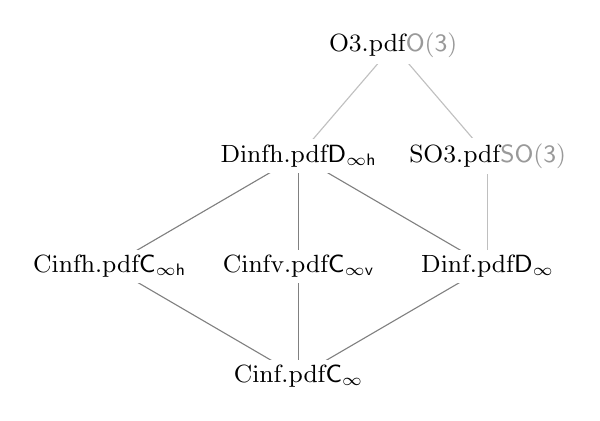
\begin{tikzpicture}[x=1cm, y=1cm, every node/.style={fill=white, font=\small, inner sep=2pt}]
\draw[black!50, line width=0.4pt] (0,0) -- (-2.4,1.4);
\draw[black!50, line width=0.4pt] (0,0) -- (0,1.4);
\draw[black!50, line width=0.4pt] (0,0) -- (2.4,1.4);
\draw[black!50, line width=0.4pt] (-2.4,1.4) -- (0,2.8);
\draw[black!50, line width=0.4pt] (0,1.4) -- (0,2.8);
\draw[black!50, line width=0.4pt] (2.4,1.4) -- (0,2.8);
\draw[black!25, line width=0.4pt] (2.4,1.4) -- (2.4,2.8);
\draw[black!25, line width=0.4pt] (0,2.8) -- (1.2,4.2);
\draw[black!25, line width=0.4pt] (2.4,2.8) -- (1.2,4.2);
\node at (0,0) {\href{Cinf.pdf}{\textcolor{black}{$\grp{C_{\infty}}$}}};
\node at (-2.4,1.4) {\href{Cinfh.pdf}{\textcolor{black}{$\grp{C_{\infty h}}$}}};
\node at (0,1.4) {\href{Cinfv.pdf}{\textcolor{black}{$\grp{C_{\infty v}}$}}};
\node at (2.4,1.4) {\href{Dinf.pdf}{\textcolor{black}{$\grp{D_{\infty}}$}}};
\node at (0,2.8) {\href{Dinfh.pdf}{\textcolor{black}{$\grp{D_{\infty h}}$}}};
\node at (2.4,2.8) {\href{SO3.pdf}{\textcolor{black!40}{$\grp{SO(3)}$}}};
\node at (1.2,4.2) {\href{O3.pdf}{\textcolor{black!40}{$\grp{O(3)}$}}};
\end{tikzpicture}\end{center}
\leavevmode\label{n:group.H}The table lists the closed subgroups $\grp{H}$ other than $\grp{D_{\infty h}}$ up to conjugacy in $\grp{D_{\infty h}}$, one per row: the continuous subgroups, then, per family, its members, a row whose symbol holds $N$ standing for every $N$ of its range, its entries functions of $N$ (members of different families are not conjugate in $\grp{D_{\infty h}}$, also where they lie in one \href{O3.pdf}{$\grp{O(3)}$} class). \label{n:group.normalizer}\label{n:group.centralizer}\label{n:head.subgroup}\label{n:head.order}\label{n:head.conjugates}\label{n:head.normal}\label{n:head.components}In the table, subgrp is $\grp{H}$, order its order, conjugates the number of subgroups conjugate to $\grp{H}$ in $\grp{D_{\infty h}}$ and normal whether $\grp{H}$ is normal, and $\grp{N}_{\hairsp \grp{D_{\infty h}}}(\grp{H})$ and $\grp{C}_{\hairsp \grp{D_{\infty h}}}(\grp{H})$ are its normalizer and its centralizer in $\grp{D_{\infty h}}$ (\texttt{normalizer}, \texttt{centralizer}); components lists the components of the class space (section~\ref{s:class_space}) that it meets. A subgroup's other names in its class of \href{O3.pdf}{$\grp{O(3)}$} follow $\samecls$ (\href{../../CONVENTIONS.pdf}{CONVENTIONS.pdf}, section \href{../../CONVENTIONS.pdf\#conv.2.1}{2.1}).
{\small\setlength{\fillwidth}{\textwidth}\addtolength{\fillwidth}{-12\tabcolsep}\setlength{\colwidth}{0pt}\cellmax{$\grp{C_{1h}}$ $\samecls$ $\grp{C_{s}}$ $\samecls$ $\grp{C_{1v}}$}\cellmax{$\grp{C_{1v}}$ $\samecls$ $\grp{C_{s}}$ $\samecls$ $\grp{C_{1h}}$}\cellmax{$\grp{C_{2h}}$ $\samecls$ $\grp{D_{1d}}$}\cellmax{$\grp{C_{2v}}$ $\samecls$ $\grp{D_{1h}}$}\cellmax{$\grp{D_{1d}}$ $\samecls$ $\grp{C_{2h}}$}\cellmax{$\grp{D_{1h}}$ $\samecls$ $\grp{C_{2v}}$}\cellmax{$\grp{C_{\infty h}}$ $\samecls$ $\grp{S_{\infty}}$}\cellmax{$\grp{C_{\mathnormal{N}h}}$, $N \ge 3$}\cellmax{$\grp{C_{\mathnormal{N}v}}$, $N \ge 3$}\cellmax{$\grp{D_{\mathnormal{N}d}}$, $N \ge 2$}\cellmax{$\grp{D_{\mathnormal{N}h}}$, $N \ge 3$}\cellmax{$\grp{S_{2\mathnormal{N}}}$, $N \ge 2$}\cellmax{$\grp{C_{2}}$ $\samecls$ $\grp{D_{1}}$}\cellmax{$\grp{C_{\mathnormal{N}}}$, $N \ge 3$}\cellmax{$\grp{D_{1}}$ $\samecls$ $\grp{C_{2}}$}\cellmax{$\grp{D_{\mathnormal{N}}}$, $N \ge 3$}\cellmax{$\grp{S_{2}}$ $\samecls$ $\grp{C_{i}}$}\cellmax{subgrp}\cellmax{$\grp{C_{\infty v}}$}\cellmax{$\grp{D_{2h}}$}\cellmax{$\grp{C_{1}}$}\cellmax{$\grp{C_{\infty}}$}\cellmax{$\grp{D_{2}}$}\cellmax{$\grp{D_{\infty}}$}\addtolength{\fillwidth}{-\colwidth}\setlength{\colwidth}{0pt}\cellmax{order}\cellmax{$2N$}\cellmax{$4N$}\cellmax{$N$}\cellmax{$\infty$}\cellmax{1}\cellmax{2}\cellmax{4}\cellmax{8}\addtolength{\fillwidth}{-\colwidth}\setlength{\colwidth}{0pt}\cellmax{conjugates}\cellmax{$\infty$}\cellmax{1}\addtolength{\fillwidth}{-\colwidth}\setlength{\colwidth}{0pt}\cellmax{normal}\cellmax{yes}\cellmax{no}\addtolength{\fillwidth}{-\colwidth}\setlength{\colwidth}{0pt}\cellmax{$\grp{N}_{\hairsp \grp{D_{\infty h}}}(\grp{H})$}\cellmax{$\grp{D_{2\mathnormal{N}h}}$}\cellmax{$\grp{D_{2h}}$}\cellmax{$\grp{D_{4h}}$}\cellmax{$\grp{D_{\infty h}}$}\addtolength{\fillwidth}{-\colwidth}\setlength{\colwidth}{0pt}\cellmax{$\grp{C}_{\hairsp \grp{D_{\infty h}}}(\grp{H})$}\cellmax{$\grp{C_{2h}}$}\cellmax{$\grp{C_{\infty h}}$}\cellmax{$\grp{D_{2h}}$}\cellmax{$\grp{D_{\infty h}}$}\addtolength{\fillwidth}{-\colwidth}\setlength{\colwidth}{0pt}\cellmax{$\comp{C_{\infty}(\phi)}$, $\comp{\infty C_2'}$, $\comp{i\,C_{\infty}(\phi)}$, $\comp{\infty\sigma_v}$}\cellmax{$\comp{C_{\infty}(\phi)}$, $\comp{i\,C_{\infty}(\phi)}$}\cellmax{$\comp{C_{\infty}(\phi)}$, $\comp{\infty C_2'}$}\cellmax{components}\cellmax{$\comp{C_{\infty}(\phi)}$, $\comp{\infty\sigma_v}$}\cellmax{$\comp{C_{\infty}(\phi)}$}\fillcap\begin{longtable}{@{}lrrlll>{\RaggedRight\arraybackslash}p{\fillwidth}@{}}\toprule
subgrp & order & conjugates & normal & $\grp{N}_{\hairsp \grp{D_{\infty h}}}(\grp{H})$ & $\grp{C}_{\hairsp \grp{D_{\infty h}}}(\grp{H})$ & components\\\midrule\endhead
\bottomrule\endfoot\endlastfoot
\href{Cinf.pdf}{$\grp{C_{\infty}}$} & $\infty$ & 1 & yes & \href{Dinfh.pdf}{$\grp{D_{\infty h}}$} & \href{Cinfh.pdf}{$\grp{C_{\infty h}}$} & $\comp{C_{\infty}(\phi)}$\\*
\href{Cinfh.pdf}{$\grp{C_{\infty h}}$} $\samecls$ \href{Cinfh.pdf}{$\grp{S_{\infty}}$} & $\infty$ & 1 & yes & \href{Dinfh.pdf}{$\grp{D_{\infty h}}$} & \href{Cinfh.pdf}{$\grp{C_{\infty h}}$} & $\comp{C_{\infty}(\phi)}$, $\comp{i\,C_{\infty}(\phi)}$\\
\href{Cinfv.pdf}{$\grp{C_{\infty v}}$} & $\infty$ & 1 & yes & \href{Dinfh.pdf}{$\grp{D_{\infty h}}$} & \href{C2h.pdf}{$\grp{C_{2h}}$} & $\comp{C_{\infty}(\phi)}$, $\comp{\infty\sigma_v}$\\
\href{Dinf.pdf}{$\grp{D_{\infty}}$} & $\infty$ & 1 & yes & \href{Dinfh.pdf}{$\grp{D_{\infty h}}$} & \href{C2h.pdf}{$\grp{C_{2h}}$} & $\comp{C_{\infty}(\phi)}$, $\comp{\infty C_2'}$\\
\grouprule{0pt}{\lightrulewidth}
\href{C1.pdf}{$\grp{C_{1}}$} & 1 & 1 & yes & \href{Dinfh.pdf}{$\grp{D_{\infty h}}$} & \href{Dinfh.pdf}{$\grp{D_{\infty h}}$} & $\comp{C_{\infty}(\phi)}$\\
\href{C2.pdf}{$\grp{C_{2}}$} $\samecls$ \href{D1.pdf}{$\grp{D_{1}}$} & 2 & 1 & yes & \href{Dinfh.pdf}{$\grp{D_{\infty h}}$} & \href{Dinfh.pdf}{$\grp{D_{\infty h}}$} & $\comp{C_{\infty}(\phi)}$\\
$\grp{C_{\mathnormal{N}}}$, $N \ge 3$ & $N$ & 1 & yes & \href{Dinfh.pdf}{$\grp{D_{\infty h}}$} & \href{Cinfh.pdf}{$\grp{C_{\infty h}}$} & $\comp{C_{\infty}(\phi)}$\\
\grouprule{0pt}{\lightrulewidth}
\href{S2.pdf}{$\grp{S_{2}}$} $\samecls$ \href{S2.pdf}{$\grp{C_{i}}$} & 2 & 1 & yes & \href{Dinfh.pdf}{$\grp{D_{\infty h}}$} & \href{Dinfh.pdf}{$\grp{D_{\infty h}}$} & $\comp{C_{\infty}(\phi)}$, $\comp{i\,C_{\infty}(\phi)}$\\
$\grp{S_{2\mathnormal{N}}}$, $N \ge 2$ & $2N$ & 1 & yes & \href{Dinfh.pdf}{$\grp{D_{\infty h}}$} & \href{Cinfh.pdf}{$\grp{C_{\infty h}}$} & $\comp{C_{\infty}(\phi)}$, $\comp{i\,C_{\infty}(\phi)}$\\
\grouprule{0pt}{\lightrulewidth}
\href{C1h.pdf}{$\grp{C_{1h}}$} $\samecls$ \href{C1v.pdf}{$\grp{C_{s}}$} $\samecls$ \href{C1v.pdf}{$\grp{C_{1v}}$} & 2 & 1 & yes & \href{Dinfh.pdf}{$\grp{D_{\infty h}}$} & \href{Dinfh.pdf}{$\grp{D_{\infty h}}$} & $\comp{C_{\infty}(\phi)}$, $\comp{i\,C_{\infty}(\phi)}$\\
\href{C2h.pdf}{$\grp{C_{2h}}$} $\samecls$ \href{D1d.pdf}{$\grp{D_{1d}}$} & 4 & 1 & yes & \href{Dinfh.pdf}{$\grp{D_{\infty h}}$} & \href{Dinfh.pdf}{$\grp{D_{\infty h}}$} & $\comp{C_{\infty}(\phi)}$, $\comp{i\,C_{\infty}(\phi)}$\\
$\grp{C_{\mathnormal{N}h}}$, $N \ge 3$ & $2N$ & 1 & yes & \href{Dinfh.pdf}{$\grp{D_{\infty h}}$} & \href{Cinfh.pdf}{$\grp{C_{\infty h}}$} & $\comp{C_{\infty}(\phi)}$, $\comp{i\,C_{\infty}(\phi)}$\\
\grouprule{0pt}{\lightrulewidth}
\href{C1v.pdf}{$\grp{C_{1v}}$} $\samecls$ \href{C1v.pdf}{$\grp{C_{s}}$} $\samecls$ \href{C1h.pdf}{$\grp{C_{1h}}$} & 2 & $\infty$ & no & \href{D2h.pdf}{$\grp{D_{2h}}$} & \href{D2h.pdf}{$\grp{D_{2h}}$} & $\comp{C_{\infty}(\phi)}$, $\comp{\infty\sigma_v}$\\
\href{C2v.pdf}{$\grp{C_{2v}}$} $\samecls$ \href{D1h.pdf}{$\grp{D_{1h}}$} & 4 & $\infty$ & no & \href{D4h.pdf}{$\grp{D_{4h}}$} & \href{D2h.pdf}{$\grp{D_{2h}}$} & $\comp{C_{\infty}(\phi)}$, $\comp{\infty\sigma_v}$\\
$\grp{C_{\mathnormal{N}v}}$, $N \ge 3$ & $2N$ & $\infty$ & no & $\grp{D_{2\mathnormal{N}h}}$ & \href{C2h.pdf}{$\grp{C_{2h}}$} & $\comp{C_{\infty}(\phi)}$, $\comp{\infty\sigma_v}$\\
\grouprule{0pt}{\lightrulewidth}
\href{D1.pdf}{$\grp{D_{1}}$} $\samecls$ \href{C2.pdf}{$\grp{C_{2}}$} & 2 & $\infty$ & no & \href{D2h.pdf}{$\grp{D_{2h}}$} & \href{D2h.pdf}{$\grp{D_{2h}}$} & $\comp{C_{\infty}(\phi)}$, $\comp{\infty C_2'}$\\
\href{D2.pdf}{$\grp{D_{2}}$} & 4 & $\infty$ & no & \href{D4h.pdf}{$\grp{D_{4h}}$} & \href{D2h.pdf}{$\grp{D_{2h}}$} & $\comp{C_{\infty}(\phi)}$, $\comp{\infty C_2'}$\\
$\grp{D_{\mathnormal{N}}}$, $N \ge 3$ & $2N$ & $\infty$ & no & $\grp{D_{2\mathnormal{N}h}}$ & \href{C2h.pdf}{$\grp{C_{2h}}$} & $\comp{C_{\infty}(\phi)}$, $\comp{\infty C_2'}$\\
\grouprule{0pt}{\lightrulewidth}
\href{D1h.pdf}{$\grp{D_{1h}}$} $\samecls$ \href{C2v.pdf}{$\grp{C_{2v}}$} & 4 & $\infty$ & no & \href{D2h.pdf}{$\grp{D_{2h}}$} & \href{D2h.pdf}{$\grp{D_{2h}}$} & $\comp{C_{\infty}(\phi)}$, $\comp{\infty C_2'}$, $\comp{i\,C_{\infty}(\phi)}$, $\comp{\infty\sigma_v}$\\
\href{D2h.pdf}{$\grp{D_{2h}}$} & 8 & $\infty$ & no & \href{D4h.pdf}{$\grp{D_{4h}}$} & \href{D2h.pdf}{$\grp{D_{2h}}$} & $\comp{C_{\infty}(\phi)}$, $\comp{\infty C_2'}$, $\comp{i\,C_{\infty}(\phi)}$, $\comp{\infty\sigma_v}$\\
$\grp{D_{\mathnormal{N}h}}$, $N \ge 3$ & $4N$ & $\infty$ & no & $\grp{D_{2\mathnormal{N}h}}$ & \href{C2h.pdf}{$\grp{C_{2h}}$} & $\comp{C_{\infty}(\phi)}$, $\comp{\infty C_2'}$, $\comp{i\,C_{\infty}(\phi)}$, $\comp{\infty\sigma_v}$\\
\grouprule{0pt}{\lightrulewidth}
\href{D1d.pdf}{$\grp{D_{1d}}$} $\samecls$ \href{C2h.pdf}{$\grp{C_{2h}}$} & 4 & $\infty$ & no & \href{D2h.pdf}{$\grp{D_{2h}}$} & \href{D2h.pdf}{$\grp{D_{2h}}$} & $\comp{C_{\infty}(\phi)}$, $\comp{\infty C_2'}$, $\comp{i\,C_{\infty}(\phi)}$, $\comp{\infty\sigma_v}$\\*
$\grp{D_{\mathnormal{N}d}}$, $N \ge 2$ & $4N$ & $\infty$ & no & $\grp{D_{2\mathnormal{N}h}}$ & \href{C2h.pdf}{$\grp{C_{2h}}$} & $\comp{C_{\infty}(\phi)}$, $\comp{\infty C_2'}$, $\comp{i\,C_{\infty}(\phi)}$, $\comp{\infty\sigma_v}$\\
\bottomrule\end{longtable}}
\needspace{103pt}
\section{Descent of symmetry}\label{s:subduction}
Conventions: \href{../../CONVENTIONS.pdf}{CONVENTIONS.pdf}, section \href{../../CONVENTIONS.pdf\#conv.16.1}{16.1}.
The closed subgroups of $\grp{D_{\infty h}}$ other than $\grp{D_{\infty h}}$, up to conjugacy in $\grp{D_{\infty h}}$, are its continuous subgroups and, for every $N \ge 1$, one subgroup per member of each family of section~\ref{s:subgroups}: the group of that member's document, in its own frame. Members of different families are not conjugate in $\grp{D_{\infty h}}$, also where they lie in one \href{O3.pdf}{$\grp{O(3)}$} class, such as \href{D1.pdf}{$\grp{D_{1}}$} and \href{C2.pdf}{$\grp{C_{2}}$} (a binary axis perpendicular to $z$ and along $z$). The entry of row $\Gamma$ is $\restr{\Gamma}{\grp{H}}$ as a sum of the irreps of $\grp{H}$.
\needspace{149pt}
\paragraph{Continuous subgroups.} \label{n:head.index.subgroup}The row subgrp gives each continuous subgroup $\grp{H}$ and the row index its index $\grpindex{\grp{D_{\infty h}}}{\grp{H}}$. The intertwiners, in the rotation-diagonal basis $(\ket{e_1}, \ket{e_2})$ of a family of dimension 2, are the identity, except: to \href{Cinf.pdf}{$\grp{C_{\infty}}$} and \href{Cinfh.pdf}{$\grp{C_{\infty h}}$}, the exchange of $\ket{e_1}$ and $\ket{e_2}$ of $\irr{e}_{n,\ptag{g}}$ and $\irr{e}_{n,\ptag{u}}$; to \href{Dinf.pdf}{$\grp{D_{\infty}}$}, the sign $(-1)^n$ on $\ket{e_2}$ of $\irr{e}_{n,\ptag{g}}$ and $(-1)^{n+1}$ on that of $\irr{e}_{n,\ptag{u}}$ (\texttt{subduction\symbol{95}subgroups.continuous[]}).
{\small\begin{longtable}{@{}lcccc@{}}\toprule
subgrp & \href{Cinf.pdf}{$\grp{C_{\infty}}$} & \href{Cinfh.pdf}{$\grp{C_{\infty h}}$} & \href{Cinfv.pdf}{$\grp{C_{\infty v}}$} & \href{Dinf.pdf}{$\grp{D_{\infty}}$}\\
index & 4 & 2 & 2 & 2\\\midrule\endhead
\bottomrule\endfoot\endlastfoot
$\irr{a}_{1\ptag{g}}$ & $\irr{a}$ & $\irr{a}_{\ptag{g}}$ & $\irr{a}_{1}$ & $\irr{a}_{1}$\\*
$\irr{a}_{2\ptag{g}}$ & $\irr{a}$ & $\irr{a}_{\ptag{g}}$ & $\irr{a}_{2}$ & $\irr{a}_{2}$\\*
$\irr{e}_{n,\ptag{g}}$ & $\conjpair{1}\irr{e}_{n}\oplus \conjpair{2}\irr{e}_{n}$ & $\conjpair{1}\irr{e}_{n,\ptag{g}}\oplus \conjpair{2}\irr{e}_{n,\ptag{g}}$ & $\irr{e}_{n}$ & $\irr{e}_{n}$\\*
$\irr{a}_{1\ptag{u}}$ & $\irr{a}$ & $\irr{a}_{\ptag{u}}$ & $\irr{a}_{2}$ & $\irr{a}_{1}$\\*
$\irr{a}_{2\ptag{u}}$ & $\irr{a}$ & $\irr{a}_{\ptag{u}}$ & $\irr{a}_{1}$ & $\irr{a}_{2}$\\*
$\irr{e}_{n,\ptag{u}}$ & $\conjpair{1}\irr{e}_{n}\oplus \conjpair{2}\irr{e}_{n}$ & $\conjpair{1}\irr{e}_{n,\ptag{u}}\oplus \conjpair{2}\irr{e}_{n,\ptag{u}}$ & $\irr{e}_{n}$ & $\irr{e}_{n}$\\
\bottomrule\end{longtable}}
\needspace{116pt}
\paragraph{Finite subgroups.} \label{n:function.character.plain}\label{n:element.principal}\label{n:constant.root}\label{n:index.residue}\label{n:index.order.principal}For each family, the rule gives the restriction for every $N$ as the label of \href{../../CONVENTIONS.pdf}{CONVENTIONS.pdf}, section \href{../../CONVENTIONS.pdf\#conv.6.1}{6.1}, of the irrep with $\chi(g_p) = \rootunity{N_p}^{q}$ (the pair $\rootunity{N_p}^{\pm q}$ for an $\irr{e}_n$), $\rootunity{N_p} = \expe^{2\pi\iunit/N_p}$, where $g_p = \elt{C_\infty}(2\pi/N)$ and $N_p = N$, or $g_p = \elt{\sigma_h C_\infty}(\pi/N)$ and $N_p = 2N$ in $\grp{S_{2\mathnormal{N}}}$ and in $\grp{D_{\mathnormal{N}d}}$ with $N$ even; for $N = 1$ and $2$ the labels take the names of \href{../../CONVENTIONS.pdf}{CONVENTIONS.pdf}, section \href{../../CONVENTIONS.pdf\#conv.6.3}{6.3}. \label{n:index.period}The tables list $N \le 12$ and $n \le 6$; the restriction of the instance $n$ depends on $n$ only modulo the period $\period$ of the member, and the JSON lists $n = 1, 2, \dots, \period$ with the intertwiners (\texttt{subduction\symbol{95}subgroups.finite[]}). \label{n:group.normalizer.o3}\label{n:group.centralizer.o3}\label{n:element.h}The record of $\grp{H}$ maps onto the subgroup in $\grpindex{\grp{N}}{\grp{C}}$ ways, $h \mapsto g h g^{-1}$ ($h \in \grp{H}$) for the $g \in \grp{O(3)}$ that carry $\grp{H}$ to it, $\grp{N}$ and $\grp{C}$ the normalizer and the centralizer of $\grp{H}$ in \href{O3.pdf}{$\grp{O(3)}$}; the row centralizer of section Names and structure of the document of $\grp{H}$ gives $\grp{C}$ and this index (the index in the row normalizer is $\grpindex{\grp{N}}{\grp{H}}$). Two maps related by a conjugation in $\grp{D_{\infty h}}$ give the same restriction, so the maps fall into $\grpindex{\grp{N}}{\grp{C}}/\grpindex{\grp{N}_{\hairsp \grp{D_{\infty h}}}}{\grp{C}_{\hairsp \grp{D_{\infty h}}}}$ classes, $\grp{N}_{\hairsp \grp{D_{\infty h}}}$ and $\grp{C}_{\hairsp \grp{D_{\infty h}}}$ the normalizer and the centralizer of the subgroup in $\grp{D_{\infty h}}$ (the table of section~\ref{s:subgroups}). \label{n:head.setting}A subgroup whose classes give different tables has one column per table, its settings: 1 for the stored monomorphism (\texttt{monomorphism}) and 2, 3, \dots{} for the \texttt{alternative\symbol{95}settings}, each with the images of the generators of $\grp{H}$ (\texttt{setting}). \label{n:head.images}\label{n:element.generator.index}The row images gives, under each setting, each generator of $\grp{H}$ whose image differs between the settings, in their order, by the symbol of its class (\href{../../CONVENTIONS.pdf}{CONVENTIONS.pdf}, section \href{../../CONVENTIONS.pdf\#conv.5.1}{5.1}), mapped to its image, the element of its component of the class space at its angle; where two generators share a symbol, a superscript number in brackets gives the generator's index in the document of $\grp{H}$. \label{n:irrep.Delta}Each other column under a subgroup is column 1 with each irrep $\Lambda$ of $\grp{H}$ replaced by $\Lambda$ composed with one automorphism of $\grp{H}$ that a conjugation in \href{O3.pdf}{$\grp{O(3)}$} induces and none in $\grp{D_{\infty h}}$ does (\href{../../CONVENTIONS.pdf}{CONVENTIONS.pdf}, section \href{../../CONVENTIONS.pdf\#conv.12.1}{12.1}).
\needspace{95pt}
\paragraph{Subduction to the $\grp{C_{\mathnormal{N}}}$ family.}
{\small\setlength{\fillwidth}{\textwidth}\addtolength{\fillwidth}{-2\tabcolsep}\setlength{\colwidth}{0pt}\cellmax{$\irr{e}_{n,\ptag{g}}$}\cellmax{$\irr{e}_{n,\ptag{u}}$}\cellmax{$\irr{a}_{1\ptag{g}}$}\cellmax{$\irr{a}_{1\ptag{u}}$}\cellmax{$\irr{a}_{2\ptag{g}}$}\cellmax{$\irr{a}_{2\ptag{u}}$}\addtolength{\fillwidth}{-\colwidth}\setlength{\colwidth}{0pt}\cellmax{$2\,\irr{a}$ if $q = 0$, $2\,\irr{b}$ if $q = N/2$, $\conjpair{1}\irr{e}_{\min(q, N-q)}\oplus \conjpair{2}\irr{e}_{\min(q, N-q)}$ otherwise; $q = n \bmod N$}\cellmax{$\irr{a}$}\fillcap\begin{longtable}{@{}l>{\raggedright\arraybackslash}p{\fillwidth}@{}}\toprule
\multicolumn{2}{@{}c@{}}{every $N$}\\*
$\irr{a}_{1\ptag{g}}$ & $\irr{a}$\\*
$\irr{a}_{2\ptag{g}}$ & $\irr{a}$\\*
$\irr{e}_{n,\ptag{g}}$ & $2\,\irr{a}$ if $q = 0$, $2\,\irr{b}$ if $q = N/2$, $\conjpair{1}\irr{e}_{\min(q, N-q)}\oplus \conjpair{2}\irr{e}_{\min(q, N-q)}$ otherwise; $q = n \bmod N$\\*
$\irr{a}_{1\ptag{u}}$ & $\irr{a}$\\*
$\irr{a}_{2\ptag{u}}$ & $\irr{a}$\\*
$\irr{e}_{n,\ptag{u}}$ & $2\,\irr{a}$ if $q = 0$, $2\,\irr{b}$ if $q = N/2$, $\conjpair{1}\irr{e}_{\min(q, N-q)}\oplus \conjpair{2}\irr{e}_{\min(q, N-q)}$ otherwise; $q = n \bmod N$\\
\bottomrule\end{longtable}}
{\small\begin{longtable}{@{}lcccccccc@{}}\toprule
subgrp & \href{C2.pdf}{$\grp{C_{2}}$} & \href{C3.pdf}{$\grp{C_{3}}$} & \href{C4.pdf}{$\grp{C_{4}}$} & \href{C5.pdf}{$\grp{C_{5}}$} & \href{C6.pdf}{$\grp{C_{6}}$} & \href{C7.pdf}{$\grp{C_{7}}$} & \href{C8.pdf}{$\grp{C_{8}}$} & \href{C9.pdf}{$\grp{C_{9}}$}\\\midrule\endhead
\bottomrule\endfoot\endlastfoot
$\irr{a}_{1\ptag{g}}$ & $\irr{a}$ & $\irr{a}$ & $\irr{a}$ & $\irr{a}$ & $\irr{a}$ & $\irr{a}$ & $\irr{a}$ & $\irr{a}$\\*
$\irr{a}_{2\ptag{g}}$ & $\irr{a}$ & $\irr{a}$ & $\irr{a}$ & $\irr{a}$ & $\irr{a}$ & $\irr{a}$ & $\irr{a}$ & $\irr{a}$\\
$\irr{e}_{1\ptag{g}}$ & $2\,\irr{b}$ & $\conjpair{1}\irr{e}\oplus \conjpair{2}\irr{e}$ & $\conjpair{1}\irr{e}\oplus \conjpair{2}\irr{e}$ & $\conjpair{1}\irr{e}_{1}\oplus \conjpair{2}\irr{e}_{1}$ & $\conjpair{1}\irr{e}_{1}\oplus \conjpair{2}\irr{e}_{1}$ & $\conjpair{1}\irr{e}_{1}\oplus \conjpair{2}\irr{e}_{1}$ & $\conjpair{1}\irr{e}_{1}\oplus \conjpair{2}\irr{e}_{1}$ & $\conjpair{1}\irr{e}_{1}\oplus \conjpair{2}\irr{e}_{1}$\\
$\irr{e}_{2\ptag{g}}$ & $2\,\irr{a}$ & $\conjpair{1}\irr{e}\oplus \conjpair{2}\irr{e}$ & $2\,\irr{b}$ & $\conjpair{1}\irr{e}_{2}\oplus \conjpair{2}\irr{e}_{2}$ & $\conjpair{1}\irr{e}_{2}\oplus \conjpair{2}\irr{e}_{2}$ & $\conjpair{1}\irr{e}_{2}\oplus \conjpair{2}\irr{e}_{2}$ & $\conjpair{1}\irr{e}_{2}\oplus \conjpair{2}\irr{e}_{2}$ & $\conjpair{1}\irr{e}_{2}\oplus \conjpair{2}\irr{e}_{2}$\\
$\irr{e}_{3\ptag{g}}$ & $2\,\irr{b}$ & $2\,\irr{a}$ & $\conjpair{1}\irr{e}\oplus \conjpair{2}\irr{e}$ & $\conjpair{1}\irr{e}_{2}\oplus \conjpair{2}\irr{e}_{2}$ & $2\,\irr{b}$ & $\conjpair{1}\irr{e}_{3}\oplus \conjpair{2}\irr{e}_{3}$ & $\conjpair{1}\irr{e}_{3}\oplus \conjpair{2}\irr{e}_{3}$ & $\conjpair{1}\irr{e}_{3}\oplus \conjpair{2}\irr{e}_{3}$\\
$\irr{e}_{4\ptag{g}}$ & $2\,\irr{a}$ & $\conjpair{1}\irr{e}\oplus \conjpair{2}\irr{e}$ & $2\,\irr{a}$ & $\conjpair{1}\irr{e}_{1}\oplus \conjpair{2}\irr{e}_{1}$ & $\conjpair{1}\irr{e}_{2}\oplus \conjpair{2}\irr{e}_{2}$ & $\conjpair{1}\irr{e}_{3}\oplus \conjpair{2}\irr{e}_{3}$ & $2\,\irr{b}$ & $\conjpair{1}\irr{e}_{4}\oplus \conjpair{2}\irr{e}_{4}$\\
$\irr{e}_{5\ptag{g}}$ & $2\,\irr{b}$ & $\conjpair{1}\irr{e}\oplus \conjpair{2}\irr{e}$ & $\conjpair{1}\irr{e}\oplus \conjpair{2}\irr{e}$ & $2\,\irr{a}$ & $\conjpair{1}\irr{e}_{1}\oplus \conjpair{2}\irr{e}_{1}$ & $\conjpair{1}\irr{e}_{2}\oplus \conjpair{2}\irr{e}_{2}$ & $\conjpair{1}\irr{e}_{3}\oplus \conjpair{2}\irr{e}_{3}$ & $\conjpair{1}\irr{e}_{4}\oplus \conjpair{2}\irr{e}_{4}$\\
$\irr{e}_{6\ptag{g}}$ & $2\,\irr{a}$ & $2\,\irr{a}$ & $2\,\irr{b}$ & $\conjpair{1}\irr{e}_{1}\oplus \conjpair{2}\irr{e}_{1}$ & $2\,\irr{a}$ & $\conjpair{1}\irr{e}_{1}\oplus \conjpair{2}\irr{e}_{1}$ & $\conjpair{1}\irr{e}_{2}\oplus \conjpair{2}\irr{e}_{2}$ & $\conjpair{1}\irr{e}_{3}\oplus \conjpair{2}\irr{e}_{3}$\\
$\irr{a}_{1\ptag{u}}$ & $\irr{a}$ & $\irr{a}$ & $\irr{a}$ & $\irr{a}$ & $\irr{a}$ & $\irr{a}$ & $\irr{a}$ & $\irr{a}$\\
$\irr{a}_{2\ptag{u}}$ & $\irr{a}$ & $\irr{a}$ & $\irr{a}$ & $\irr{a}$ & $\irr{a}$ & $\irr{a}$ & $\irr{a}$ & $\irr{a}$\\
$\irr{e}_{1\ptag{u}}$ & $2\,\irr{b}$ & $\conjpair{1}\irr{e}\oplus \conjpair{2}\irr{e}$ & $\conjpair{1}\irr{e}\oplus \conjpair{2}\irr{e}$ & $\conjpair{1}\irr{e}_{1}\oplus \conjpair{2}\irr{e}_{1}$ & $\conjpair{1}\irr{e}_{1}\oplus \conjpair{2}\irr{e}_{1}$ & $\conjpair{1}\irr{e}_{1}\oplus \conjpair{2}\irr{e}_{1}$ & $\conjpair{1}\irr{e}_{1}\oplus \conjpair{2}\irr{e}_{1}$ & $\conjpair{1}\irr{e}_{1}\oplus \conjpair{2}\irr{e}_{1}$\\
$\irr{e}_{2\ptag{u}}$ & $2\,\irr{a}$ & $\conjpair{1}\irr{e}\oplus \conjpair{2}\irr{e}$ & $2\,\irr{b}$ & $\conjpair{1}\irr{e}_{2}\oplus \conjpair{2}\irr{e}_{2}$ & $\conjpair{1}\irr{e}_{2}\oplus \conjpair{2}\irr{e}_{2}$ & $\conjpair{1}\irr{e}_{2}\oplus \conjpair{2}\irr{e}_{2}$ & $\conjpair{1}\irr{e}_{2}\oplus \conjpair{2}\irr{e}_{2}$ & $\conjpair{1}\irr{e}_{2}\oplus \conjpair{2}\irr{e}_{2}$\\
$\irr{e}_{3\ptag{u}}$ & $2\,\irr{b}$ & $2\,\irr{a}$ & $\conjpair{1}\irr{e}\oplus \conjpair{2}\irr{e}$ & $\conjpair{1}\irr{e}_{2}\oplus \conjpair{2}\irr{e}_{2}$ & $2\,\irr{b}$ & $\conjpair{1}\irr{e}_{3}\oplus \conjpair{2}\irr{e}_{3}$ & $\conjpair{1}\irr{e}_{3}\oplus \conjpair{2}\irr{e}_{3}$ & $\conjpair{1}\irr{e}_{3}\oplus \conjpair{2}\irr{e}_{3}$\\
$\irr{e}_{4\ptag{u}}$ & $2\,\irr{a}$ & $\conjpair{1}\irr{e}\oplus \conjpair{2}\irr{e}$ & $2\,\irr{a}$ & $\conjpair{1}\irr{e}_{1}\oplus \conjpair{2}\irr{e}_{1}$ & $\conjpair{1}\irr{e}_{2}\oplus \conjpair{2}\irr{e}_{2}$ & $\conjpair{1}\irr{e}_{3}\oplus \conjpair{2}\irr{e}_{3}$ & $2\,\irr{b}$ & $\conjpair{1}\irr{e}_{4}\oplus \conjpair{2}\irr{e}_{4}$\\
$\irr{e}_{5\ptag{u}}$ & $2\,\irr{b}$ & $\conjpair{1}\irr{e}\oplus \conjpair{2}\irr{e}$ & $\conjpair{1}\irr{e}\oplus \conjpair{2}\irr{e}$ & $2\,\irr{a}$ & $\conjpair{1}\irr{e}_{1}\oplus \conjpair{2}\irr{e}_{1}$ & $\conjpair{1}\irr{e}_{2}\oplus \conjpair{2}\irr{e}_{2}$ & $\conjpair{1}\irr{e}_{3}\oplus \conjpair{2}\irr{e}_{3}$ & $\conjpair{1}\irr{e}_{4}\oplus \conjpair{2}\irr{e}_{4}$\\*
$\irr{e}_{6\ptag{u}}$ & $2\,\irr{a}$ & $2\,\irr{a}$ & $2\,\irr{b}$ & $\conjpair{1}\irr{e}_{1}\oplus \conjpair{2}\irr{e}_{1}$ & $2\,\irr{a}$ & $\conjpair{1}\irr{e}_{1}\oplus \conjpair{2}\irr{e}_{1}$ & $\conjpair{1}\irr{e}_{2}\oplus \conjpair{2}\irr{e}_{2}$ & $\conjpair{1}\irr{e}_{3}\oplus \conjpair{2}\irr{e}_{3}$\\
\bottomrule\end{longtable}}
{\small\begin{longtable}{@{}lccc@{}}\toprule
subgrp & \href{C10.pdf}{$\grp{C_{10}}$} & \href{C11.pdf}{$\grp{C_{11}}$} & \href{C12.pdf}{$\grp{C_{12}}$}\\\midrule\endhead
\bottomrule\endfoot\endlastfoot
$\irr{a}_{1\ptag{g}}$ & $\irr{a}$ & $\irr{a}$ & $\irr{a}$\\*
$\irr{a}_{2\ptag{g}}$ & $\irr{a}$ & $\irr{a}$ & $\irr{a}$\\
$\irr{e}_{1\ptag{g}}$ & $\conjpair{1}\irr{e}_{1}\oplus \conjpair{2}\irr{e}_{1}$ & $\conjpair{1}\irr{e}_{1}\oplus \conjpair{2}\irr{e}_{1}$ & $\conjpair{1}\irr{e}_{1}\oplus \conjpair{2}\irr{e}_{1}$\\
$\irr{e}_{2\ptag{g}}$ & $\conjpair{1}\irr{e}_{2}\oplus \conjpair{2}\irr{e}_{2}$ & $\conjpair{1}\irr{e}_{2}\oplus \conjpair{2}\irr{e}_{2}$ & $\conjpair{1}\irr{e}_{2}\oplus \conjpair{2}\irr{e}_{2}$\\
$\irr{e}_{3\ptag{g}}$ & $\conjpair{1}\irr{e}_{3}\oplus \conjpair{2}\irr{e}_{3}$ & $\conjpair{1}\irr{e}_{3}\oplus \conjpair{2}\irr{e}_{3}$ & $\conjpair{1}\irr{e}_{3}\oplus \conjpair{2}\irr{e}_{3}$\\
$\irr{e}_{4\ptag{g}}$ & $\conjpair{1}\irr{e}_{4}\oplus \conjpair{2}\irr{e}_{4}$ & $\conjpair{1}\irr{e}_{4}\oplus \conjpair{2}\irr{e}_{4}$ & $\conjpair{1}\irr{e}_{4}\oplus \conjpair{2}\irr{e}_{4}$\\
$\irr{e}_{5\ptag{g}}$ & $2\,\irr{b}$ & $\conjpair{1}\irr{e}_{5}\oplus \conjpair{2}\irr{e}_{5}$ & $\conjpair{1}\irr{e}_{5}\oplus \conjpair{2}\irr{e}_{5}$\\
$\irr{e}_{6\ptag{g}}$ & $\conjpair{1}\irr{e}_{4}\oplus \conjpair{2}\irr{e}_{4}$ & $\conjpair{1}\irr{e}_{5}\oplus \conjpair{2}\irr{e}_{5}$ & $2\,\irr{b}$\\
$\irr{a}_{1\ptag{u}}$ & $\irr{a}$ & $\irr{a}$ & $\irr{a}$\\
$\irr{a}_{2\ptag{u}}$ & $\irr{a}$ & $\irr{a}$ & $\irr{a}$\\
$\irr{e}_{1\ptag{u}}$ & $\conjpair{1}\irr{e}_{1}\oplus \conjpair{2}\irr{e}_{1}$ & $\conjpair{1}\irr{e}_{1}\oplus \conjpair{2}\irr{e}_{1}$ & $\conjpair{1}\irr{e}_{1}\oplus \conjpair{2}\irr{e}_{1}$\\
$\irr{e}_{2\ptag{u}}$ & $\conjpair{1}\irr{e}_{2}\oplus \conjpair{2}\irr{e}_{2}$ & $\conjpair{1}\irr{e}_{2}\oplus \conjpair{2}\irr{e}_{2}$ & $\conjpair{1}\irr{e}_{2}\oplus \conjpair{2}\irr{e}_{2}$\\
$\irr{e}_{3\ptag{u}}$ & $\conjpair{1}\irr{e}_{3}\oplus \conjpair{2}\irr{e}_{3}$ & $\conjpair{1}\irr{e}_{3}\oplus \conjpair{2}\irr{e}_{3}$ & $\conjpair{1}\irr{e}_{3}\oplus \conjpair{2}\irr{e}_{3}$\\
$\irr{e}_{4\ptag{u}}$ & $\conjpair{1}\irr{e}_{4}\oplus \conjpair{2}\irr{e}_{4}$ & $\conjpair{1}\irr{e}_{4}\oplus \conjpair{2}\irr{e}_{4}$ & $\conjpair{1}\irr{e}_{4}\oplus \conjpair{2}\irr{e}_{4}$\\
$\irr{e}_{5\ptag{u}}$ & $2\,\irr{b}$ & $\conjpair{1}\irr{e}_{5}\oplus \conjpair{2}\irr{e}_{5}$ & $\conjpair{1}\irr{e}_{5}\oplus \conjpair{2}\irr{e}_{5}$\\*
$\irr{e}_{6\ptag{u}}$ & $\conjpair{1}\irr{e}_{4}\oplus \conjpair{2}\irr{e}_{4}$ & $\conjpair{1}\irr{e}_{5}\oplus \conjpair{2}\irr{e}_{5}$ & $2\,\irr{b}$\\
\bottomrule\end{longtable}}
\needspace{95pt}
\paragraph{Subduction to the $\grp{S_{2\mathnormal{N}}}$ family.}
{\small\setlength{\fillwidth}{\textwidth}\addtolength{\fillwidth}{-2\tabcolsep}\setlength{\colwidth}{0pt}\cellmax{$\irr{e}_{n,\ptag{g}}$}\cellmax{$\irr{e}_{n,\ptag{u}}$}\cellmax{$\irr{a}_{1\ptag{g}}$}\cellmax{$\irr{a}_{1\ptag{u}}$}\cellmax{$\irr{a}_{2\ptag{g}}$}\cellmax{$\irr{a}_{2\ptag{u}}$}\addtolength{\fillwidth}{-\colwidth}\setlength{\colwidth}{0pt}\cellmax{$2\,\irr{a}$ if $q = 0$, $2\,\irr{b}$ if $q = N$, $\conjpair{1}\irr{e}_{\min(q, 2N-q)}\oplus \conjpair{2}\irr{e}_{\min(q, 2N-q)}$ otherwise; $q = ((N+1)n + N) \bmod 2N$}\cellmax{$2\,\irr{a}$ if $q = 0$, $2\,\irr{b}$ if $q = N$, $\conjpair{1}\irr{e}_{\min(q, 2N-q)}\oplus \conjpair{2}\irr{e}_{\min(q, 2N-q)}$ otherwise; $q = (N+1)n \bmod 2N$}\cellmax{$2\,\irr{a}_{\ptag{g}}$ if $q = 0$, $\conjpair{1}\irr{e}_{\min(q, N-q),\ptag{g}}\oplus \conjpair{2}\irr{e}_{\min(q, N-q),\ptag{g}}$ otherwise; $q = n \bmod N$}\cellmax{$2\,\irr{a}_{\ptag{u}}$ if $q = 0$, $\conjpair{1}\irr{e}_{\min(q, N-q),\ptag{u}}\oplus \conjpair{2}\irr{e}_{\min(q, N-q),\ptag{u}}$ otherwise; $q = n \bmod N$}\cellmax{$\irr{a}_{\ptag{g}}$}\cellmax{$\irr{a}_{\ptag{u}}$}\cellmax{$\irr{a}$}\cellmax{$\irr{b}$}\fillcap\begin{longtable}{@{}l>{\raggedright\arraybackslash}p{\fillwidth}@{}}\toprule
\multicolumn{2}{@{}c@{}}{odd $N$}\\*
$\irr{a}_{1\ptag{g}}$ & $\irr{a}_{\ptag{g}}$\\*
$\irr{a}_{2\ptag{g}}$ & $\irr{a}_{\ptag{g}}$\\*
$\irr{e}_{n,\ptag{g}}$ & $2\,\irr{a}_{\ptag{g}}$ if $q = 0$, $\conjpair{1}\irr{e}_{\min(q, N-q),\ptag{g}}\oplus \conjpair{2}\irr{e}_{\min(q, N-q),\ptag{g}}$ otherwise; $q = n \bmod N$\\*
$\irr{a}_{1\ptag{u}}$ & $\irr{a}_{\ptag{u}}$\\*
$\irr{a}_{2\ptag{u}}$ & $\irr{a}_{\ptag{u}}$\\*
$\irr{e}_{n,\ptag{u}}$ & $2\,\irr{a}_{\ptag{u}}$ if $q = 0$, $\conjpair{1}\irr{e}_{\min(q, N-q),\ptag{u}}\oplus \conjpair{2}\irr{e}_{\min(q, N-q),\ptag{u}}$ otherwise; $q = n \bmod N$\\
\grouprule{0pt}{\lightrulewidth}
\multicolumn{2}{@{}c@{}}{even $N$}\\*
$\irr{a}_{1\ptag{g}}$ & $\irr{a}$\\*
$\irr{a}_{2\ptag{g}}$ & $\irr{a}$\\*
$\irr{e}_{n,\ptag{g}}$ & $2\,\irr{a}$ if $q = 0$, $2\,\irr{b}$ if $q = N$, $\conjpair{1}\irr{e}_{\min(q, 2N-q)}\oplus \conjpair{2}\irr{e}_{\min(q, 2N-q)}$ otherwise; $q = (N+1)n \bmod 2N$\\*
$\irr{a}_{1\ptag{u}}$ & $\irr{b}$\\*
$\irr{a}_{2\ptag{u}}$ & $\irr{b}$\\*
$\irr{e}_{n,\ptag{u}}$ & $2\,\irr{a}$ if $q = 0$, $2\,\irr{b}$ if $q = N$, $\conjpair{1}\irr{e}_{\min(q, 2N-q)}\oplus \conjpair{2}\irr{e}_{\min(q, 2N-q)}$ otherwise; $q = ((N+1)n + N) \bmod 2N$\\
\bottomrule\end{longtable}}
{\small\begin{longtable}{@{}lccccccc@{}}\toprule
subgrp & \href{S2.pdf}{$\grp{S_{2}}$} & \href{S4.pdf}{$\grp{S_{4}}$} & \href{S6.pdf}{$\grp{S_{6}}$} & \href{S8.pdf}{$\grp{S_{8}}$} & \href{S10.pdf}{$\grp{S_{10}}$} & \href{S12.pdf}{$\grp{S_{12}}$} & \href{S14.pdf}{$\grp{S_{14}}$}\\\midrule\endhead
\bottomrule\endfoot\endlastfoot
$\irr{a}_{1\ptag{g}}$ & $\irr{a}_{\ptag{g}}$ & $\irr{a}$ & $\irr{a}_{\ptag{g}}$ & $\irr{a}$ & $\irr{a}_{\ptag{g}}$ & $\irr{a}$ & $\irr{a}_{\ptag{g}}$\\*
$\irr{a}_{2\ptag{g}}$ & $\irr{a}_{\ptag{g}}$ & $\irr{a}$ & $\irr{a}_{\ptag{g}}$ & $\irr{a}$ & $\irr{a}_{\ptag{g}}$ & $\irr{a}$ & $\irr{a}_{\ptag{g}}$\\
$\irr{e}_{1\ptag{g}}$ & $2\,\irr{a}_{\ptag{g}}$ & $\conjpair{1}\irr{e}\oplus \conjpair{2}\irr{e}$ & $\conjpair{1}\irr{e}_{\ptag{g}}\oplus \conjpair{2}\irr{e}_{\ptag{g}}$ & $\conjpair{1}\irr{e}_{3}\oplus \conjpair{2}\irr{e}_{3}$ & $\conjpair{1}\irr{e}_{1\ptag{g}}\oplus \conjpair{2}\irr{e}_{1\ptag{g}}$ & $\conjpair{1}\irr{e}_{5}\oplus \conjpair{2}\irr{e}_{5}$ & $\conjpair{1}\irr{e}_{1\ptag{g}}\oplus \conjpair{2}\irr{e}_{1\ptag{g}}$\\
$\irr{e}_{2\ptag{g}}$ & $2\,\irr{a}_{\ptag{g}}$ & $2\,\irr{b}$ & $\conjpair{1}\irr{e}_{\ptag{g}}\oplus \conjpair{2}\irr{e}_{\ptag{g}}$ & $\conjpair{1}\irr{e}_{2}\oplus \conjpair{2}\irr{e}_{2}$ & $\conjpair{1}\irr{e}_{2\ptag{g}}\oplus \conjpair{2}\irr{e}_{2\ptag{g}}$ & $\conjpair{1}\irr{e}_{2}\oplus \conjpair{2}\irr{e}_{2}$ & $\conjpair{1}\irr{e}_{2\ptag{g}}\oplus \conjpair{2}\irr{e}_{2\ptag{g}}$\\
$\irr{e}_{3\ptag{g}}$ & $2\,\irr{a}_{\ptag{g}}$ & $\conjpair{1}\irr{e}\oplus \conjpair{2}\irr{e}$ & $2\,\irr{a}_{\ptag{g}}$ & $\conjpair{1}\irr{e}_{1}\oplus \conjpair{2}\irr{e}_{1}$ & $\conjpair{1}\irr{e}_{2\ptag{g}}\oplus \conjpair{2}\irr{e}_{2\ptag{g}}$ & $\conjpair{1}\irr{e}_{3}\oplus \conjpair{2}\irr{e}_{3}$ & $\conjpair{1}\irr{e}_{3\ptag{g}}\oplus \conjpair{2}\irr{e}_{3\ptag{g}}$\\
$\irr{e}_{4\ptag{g}}$ & $2\,\irr{a}_{\ptag{g}}$ & $2\,\irr{a}$ & $\conjpair{1}\irr{e}_{\ptag{g}}\oplus \conjpair{2}\irr{e}_{\ptag{g}}$ & $2\,\irr{b}$ & $\conjpair{1}\irr{e}_{1\ptag{g}}\oplus \conjpair{2}\irr{e}_{1\ptag{g}}$ & $\conjpair{1}\irr{e}_{4}\oplus \conjpair{2}\irr{e}_{4}$ & $\conjpair{1}\irr{e}_{3\ptag{g}}\oplus \conjpair{2}\irr{e}_{3\ptag{g}}$\\
$\irr{e}_{5\ptag{g}}$ & $2\,\irr{a}_{\ptag{g}}$ & $\conjpair{1}\irr{e}\oplus \conjpair{2}\irr{e}$ & $\conjpair{1}\irr{e}_{\ptag{g}}\oplus \conjpair{2}\irr{e}_{\ptag{g}}$ & $\conjpair{1}\irr{e}_{1}\oplus \conjpair{2}\irr{e}_{1}$ & $2\,\irr{a}_{\ptag{g}}$ & $\conjpair{1}\irr{e}_{1}\oplus \conjpair{2}\irr{e}_{1}$ & $\conjpair{1}\irr{e}_{2\ptag{g}}\oplus \conjpair{2}\irr{e}_{2\ptag{g}}$\\
$\irr{e}_{6\ptag{g}}$ & $2\,\irr{a}_{\ptag{g}}$ & $2\,\irr{b}$ & $2\,\irr{a}_{\ptag{g}}$ & $\conjpair{1}\irr{e}_{2}\oplus \conjpair{2}\irr{e}_{2}$ & $\conjpair{1}\irr{e}_{1\ptag{g}}\oplus \conjpair{2}\irr{e}_{1\ptag{g}}$ & $2\,\irr{b}$ & $\conjpair{1}\irr{e}_{1\ptag{g}}\oplus \conjpair{2}\irr{e}_{1\ptag{g}}$\\
$\irr{a}_{1\ptag{u}}$ & $\irr{a}_{\ptag{u}}$ & $\irr{b}$ & $\irr{a}_{\ptag{u}}$ & $\irr{b}$ & $\irr{a}_{\ptag{u}}$ & $\irr{b}$ & $\irr{a}_{\ptag{u}}$\\
$\irr{a}_{2\ptag{u}}$ & $\irr{a}_{\ptag{u}}$ & $\irr{b}$ & $\irr{a}_{\ptag{u}}$ & $\irr{b}$ & $\irr{a}_{\ptag{u}}$ & $\irr{b}$ & $\irr{a}_{\ptag{u}}$\\
$\irr{e}_{1\ptag{u}}$ & $2\,\irr{a}_{\ptag{u}}$ & $\conjpair{1}\irr{e}\oplus \conjpair{2}\irr{e}$ & $\conjpair{1}\irr{e}_{\ptag{u}}\oplus \conjpair{2}\irr{e}_{\ptag{u}}$ & $\conjpair{1}\irr{e}_{1}\oplus \conjpair{2}\irr{e}_{1}$ & $\conjpair{1}\irr{e}_{1\ptag{u}}\oplus \conjpair{2}\irr{e}_{1\ptag{u}}$ & $\conjpair{1}\irr{e}_{1}\oplus \conjpair{2}\irr{e}_{1}$ & $\conjpair{1}\irr{e}_{1\ptag{u}}\oplus \conjpair{2}\irr{e}_{1\ptag{u}}$\\
$\irr{e}_{2\ptag{u}}$ & $2\,\irr{a}_{\ptag{u}}$ & $2\,\irr{a}$ & $\conjpair{1}\irr{e}_{\ptag{u}}\oplus \conjpair{2}\irr{e}_{\ptag{u}}$ & $\conjpair{1}\irr{e}_{2}\oplus \conjpair{2}\irr{e}_{2}$ & $\conjpair{1}\irr{e}_{2\ptag{u}}\oplus \conjpair{2}\irr{e}_{2\ptag{u}}$ & $\conjpair{1}\irr{e}_{4}\oplus \conjpair{2}\irr{e}_{4}$ & $\conjpair{1}\irr{e}_{2\ptag{u}}\oplus \conjpair{2}\irr{e}_{2\ptag{u}}$\\
$\irr{e}_{3\ptag{u}}$ & $2\,\irr{a}_{\ptag{u}}$ & $\conjpair{1}\irr{e}\oplus \conjpair{2}\irr{e}$ & $2\,\irr{a}_{\ptag{u}}$ & $\conjpair{1}\irr{e}_{3}\oplus \conjpair{2}\irr{e}_{3}$ & $\conjpair{1}\irr{e}_{2\ptag{u}}\oplus \conjpair{2}\irr{e}_{2\ptag{u}}$ & $\conjpair{1}\irr{e}_{3}\oplus \conjpair{2}\irr{e}_{3}$ & $\conjpair{1}\irr{e}_{3\ptag{u}}\oplus \conjpair{2}\irr{e}_{3\ptag{u}}$\\
$\irr{e}_{4\ptag{u}}$ & $2\,\irr{a}_{\ptag{u}}$ & $2\,\irr{b}$ & $\conjpair{1}\irr{e}_{\ptag{u}}\oplus \conjpair{2}\irr{e}_{\ptag{u}}$ & $2\,\irr{a}$ & $\conjpair{1}\irr{e}_{1\ptag{u}}\oplus \conjpair{2}\irr{e}_{1\ptag{u}}$ & $\conjpair{1}\irr{e}_{2}\oplus \conjpair{2}\irr{e}_{2}$ & $\conjpair{1}\irr{e}_{3\ptag{u}}\oplus \conjpair{2}\irr{e}_{3\ptag{u}}$\\
$\irr{e}_{5\ptag{u}}$ & $2\,\irr{a}_{\ptag{u}}$ & $\conjpair{1}\irr{e}\oplus \conjpair{2}\irr{e}$ & $\conjpair{1}\irr{e}_{\ptag{u}}\oplus \conjpair{2}\irr{e}_{\ptag{u}}$ & $\conjpair{1}\irr{e}_{3}\oplus \conjpair{2}\irr{e}_{3}$ & $2\,\irr{a}_{\ptag{u}}$ & $\conjpair{1}\irr{e}_{5}\oplus \conjpair{2}\irr{e}_{5}$ & $\conjpair{1}\irr{e}_{2\ptag{u}}\oplus \conjpair{2}\irr{e}_{2\ptag{u}}$\\*
$\irr{e}_{6\ptag{u}}$ & $2\,\irr{a}_{\ptag{u}}$ & $2\,\irr{a}$ & $2\,\irr{a}_{\ptag{u}}$ & $\conjpair{1}\irr{e}_{2}\oplus \conjpair{2}\irr{e}_{2}$ & $\conjpair{1}\irr{e}_{1\ptag{u}}\oplus \conjpair{2}\irr{e}_{1\ptag{u}}$ & $2\,\irr{a}$ & $\conjpair{1}\irr{e}_{1\ptag{u}}\oplus \conjpair{2}\irr{e}_{1\ptag{u}}$\\
\bottomrule\end{longtable}}
{\small\begin{longtable}{@{}lccccc@{}}\toprule
subgrp & \href{S16.pdf}{$\grp{S_{16}}$} & \href{S18.pdf}{$\grp{S_{18}}$} & \href{S20.pdf}{$\grp{S_{20}}$} & \href{S22.pdf}{$\grp{S_{22}}$} & \href{S24.pdf}{$\grp{S_{24}}$}\\\midrule\endhead
\bottomrule\endfoot\endlastfoot
$\irr{a}_{1\ptag{g}}$ & $\irr{a}$ & $\irr{a}_{\ptag{g}}$ & $\irr{a}$ & $\irr{a}_{\ptag{g}}$ & $\irr{a}$\\*
$\irr{a}_{2\ptag{g}}$ & $\irr{a}$ & $\irr{a}_{\ptag{g}}$ & $\irr{a}$ & $\irr{a}_{\ptag{g}}$ & $\irr{a}$\\
$\irr{e}_{1\ptag{g}}$ & $\conjpair{1}\irr{e}_{7}\oplus \conjpair{2}\irr{e}_{7}$ & $\conjpair{1}\irr{e}_{1\ptag{g}}\oplus \conjpair{2}\irr{e}_{1\ptag{g}}$ & $\conjpair{1}\irr{e}_{9}\oplus \conjpair{2}\irr{e}_{9}$ & $\conjpair{1}\irr{e}_{1\ptag{g}}\oplus \conjpair{2}\irr{e}_{1\ptag{g}}$ & $\conjpair{1}\irr{e}_{11}\oplus \conjpair{2}\irr{e}_{11}$\\
$\irr{e}_{2\ptag{g}}$ & $\conjpair{1}\irr{e}_{2}\oplus \conjpair{2}\irr{e}_{2}$ & $\conjpair{1}\irr{e}_{2\ptag{g}}\oplus \conjpair{2}\irr{e}_{2\ptag{g}}$ & $\conjpair{1}\irr{e}_{2}\oplus \conjpair{2}\irr{e}_{2}$ & $\conjpair{1}\irr{e}_{2\ptag{g}}\oplus \conjpair{2}\irr{e}_{2\ptag{g}}$ & $\conjpair{1}\irr{e}_{2}\oplus \conjpair{2}\irr{e}_{2}$\\
$\irr{e}_{3\ptag{g}}$ & $\conjpair{1}\irr{e}_{5}\oplus \conjpair{2}\irr{e}_{5}$ & $\conjpair{1}\irr{e}_{3\ptag{g}}\oplus \conjpair{2}\irr{e}_{3\ptag{g}}$ & $\conjpair{1}\irr{e}_{7}\oplus \conjpair{2}\irr{e}_{7}$ & $\conjpair{1}\irr{e}_{3\ptag{g}}\oplus \conjpair{2}\irr{e}_{3\ptag{g}}$ & $\conjpair{1}\irr{e}_{9}\oplus \conjpair{2}\irr{e}_{9}$\\
$\irr{e}_{4\ptag{g}}$ & $\conjpair{1}\irr{e}_{4}\oplus \conjpair{2}\irr{e}_{4}$ & $\conjpair{1}\irr{e}_{4\ptag{g}}\oplus \conjpair{2}\irr{e}_{4\ptag{g}}$ & $\conjpair{1}\irr{e}_{4}\oplus \conjpair{2}\irr{e}_{4}$ & $\conjpair{1}\irr{e}_{4\ptag{g}}\oplus \conjpair{2}\irr{e}_{4\ptag{g}}$ & $\conjpair{1}\irr{e}_{4}\oplus \conjpair{2}\irr{e}_{4}$\\
$\irr{e}_{5\ptag{g}}$ & $\conjpair{1}\irr{e}_{3}\oplus \conjpair{2}\irr{e}_{3}$ & $\conjpair{1}\irr{e}_{4\ptag{g}}\oplus \conjpair{2}\irr{e}_{4\ptag{g}}$ & $\conjpair{1}\irr{e}_{5}\oplus \conjpair{2}\irr{e}_{5}$ & $\conjpair{1}\irr{e}_{5\ptag{g}}\oplus \conjpair{2}\irr{e}_{5\ptag{g}}$ & $\conjpair{1}\irr{e}_{7}\oplus \conjpair{2}\irr{e}_{7}$\\
$\irr{e}_{6\ptag{g}}$ & $\conjpair{1}\irr{e}_{6}\oplus \conjpair{2}\irr{e}_{6}$ & $\conjpair{1}\irr{e}_{3\ptag{g}}\oplus \conjpair{2}\irr{e}_{3\ptag{g}}$ & $\conjpair{1}\irr{e}_{6}\oplus \conjpair{2}\irr{e}_{6}$ & $\conjpair{1}\irr{e}_{5\ptag{g}}\oplus \conjpair{2}\irr{e}_{5\ptag{g}}$ & $\conjpair{1}\irr{e}_{6}\oplus \conjpair{2}\irr{e}_{6}$\\
$\irr{a}_{1\ptag{u}}$ & $\irr{b}$ & $\irr{a}_{\ptag{u}}$ & $\irr{b}$ & $\irr{a}_{\ptag{u}}$ & $\irr{b}$\\
$\irr{a}_{2\ptag{u}}$ & $\irr{b}$ & $\irr{a}_{\ptag{u}}$ & $\irr{b}$ & $\irr{a}_{\ptag{u}}$ & $\irr{b}$\\
$\irr{e}_{1\ptag{u}}$ & $\conjpair{1}\irr{e}_{1}\oplus \conjpair{2}\irr{e}_{1}$ & $\conjpair{1}\irr{e}_{1\ptag{u}}\oplus \conjpair{2}\irr{e}_{1\ptag{u}}$ & $\conjpair{1}\irr{e}_{1}\oplus \conjpair{2}\irr{e}_{1}$ & $\conjpair{1}\irr{e}_{1\ptag{u}}\oplus \conjpair{2}\irr{e}_{1\ptag{u}}$ & $\conjpair{1}\irr{e}_{1}\oplus \conjpair{2}\irr{e}_{1}$\\
$\irr{e}_{2\ptag{u}}$ & $\conjpair{1}\irr{e}_{6}\oplus \conjpair{2}\irr{e}_{6}$ & $\conjpair{1}\irr{e}_{2\ptag{u}}\oplus \conjpair{2}\irr{e}_{2\ptag{u}}$ & $\conjpair{1}\irr{e}_{8}\oplus \conjpair{2}\irr{e}_{8}$ & $\conjpair{1}\irr{e}_{2\ptag{u}}\oplus \conjpair{2}\irr{e}_{2\ptag{u}}$ & $\conjpair{1}\irr{e}_{10}\oplus \conjpair{2}\irr{e}_{10}$\\
$\irr{e}_{3\ptag{u}}$ & $\conjpair{1}\irr{e}_{3}\oplus \conjpair{2}\irr{e}_{3}$ & $\conjpair{1}\irr{e}_{3\ptag{u}}\oplus \conjpair{2}\irr{e}_{3\ptag{u}}$ & $\conjpair{1}\irr{e}_{3}\oplus \conjpair{2}\irr{e}_{3}$ & $\conjpair{1}\irr{e}_{3\ptag{u}}\oplus \conjpair{2}\irr{e}_{3\ptag{u}}$ & $\conjpair{1}\irr{e}_{3}\oplus \conjpair{2}\irr{e}_{3}$\\
$\irr{e}_{4\ptag{u}}$ & $\conjpair{1}\irr{e}_{4}\oplus \conjpair{2}\irr{e}_{4}$ & $\conjpair{1}\irr{e}_{4\ptag{u}}\oplus \conjpair{2}\irr{e}_{4\ptag{u}}$ & $\conjpair{1}\irr{e}_{6}\oplus \conjpair{2}\irr{e}_{6}$ & $\conjpair{1}\irr{e}_{4\ptag{u}}\oplus \conjpair{2}\irr{e}_{4\ptag{u}}$ & $\conjpair{1}\irr{e}_{8}\oplus \conjpair{2}\irr{e}_{8}$\\
$\irr{e}_{5\ptag{u}}$ & $\conjpair{1}\irr{e}_{5}\oplus \conjpair{2}\irr{e}_{5}$ & $\conjpair{1}\irr{e}_{4\ptag{u}}\oplus \conjpair{2}\irr{e}_{4\ptag{u}}$ & $\conjpair{1}\irr{e}_{5}\oplus \conjpair{2}\irr{e}_{5}$ & $\conjpair{1}\irr{e}_{5\ptag{u}}\oplus \conjpair{2}\irr{e}_{5\ptag{u}}$ & $\conjpair{1}\irr{e}_{5}\oplus \conjpair{2}\irr{e}_{5}$\\*
$\irr{e}_{6\ptag{u}}$ & $\conjpair{1}\irr{e}_{2}\oplus \conjpair{2}\irr{e}_{2}$ & $\conjpair{1}\irr{e}_{3\ptag{u}}\oplus \conjpair{2}\irr{e}_{3\ptag{u}}$ & $\conjpair{1}\irr{e}_{4}\oplus \conjpair{2}\irr{e}_{4}$ & $\conjpair{1}\irr{e}_{5\ptag{u}}\oplus \conjpair{2}\irr{e}_{5\ptag{u}}$ & $\conjpair{1}\irr{e}_{6}\oplus \conjpair{2}\irr{e}_{6}$\\
\bottomrule\end{longtable}}
\needspace{95pt}
\paragraph{Subduction to the $\grp{C_{\mathnormal{N}h}}$ family.}
{\small\setlength{\fillwidth}{\textwidth}\addtolength{\fillwidth}{-2\tabcolsep}\setlength{\colwidth}{0pt}\cellmax{$\irr{e}_{n,\ptag{g}}$}\cellmax{$\irr{e}_{n,\ptag{u}}$}\cellmax{$\irr{a}_{1\ptag{g}}$}\cellmax{$\irr{a}_{1\ptag{u}}$}\cellmax{$\irr{a}_{2\ptag{g}}$}\cellmax{$\irr{a}_{2\ptag{u}}$}\addtolength{\fillwidth}{-\colwidth}\setlength{\colwidth}{0pt}\cellmax{$2\,\irr{a}$ if $q = 0$, $\conjpair{1}\irr{e}_{\min(q, N-q)}\oplus \conjpair{2}\irr{e}_{\min(q, N-q)}$ otherwise; $q = n \bmod N$; the labels take $'$ for $n$ even and $''$ for $n$ odd}\cellmax{$2\,\irr{a}$ if $q = 0$, $\conjpair{1}\irr{e}_{\min(q, N-q)}\oplus \conjpair{2}\irr{e}_{\min(q, N-q)}$ otherwise; $q = n \bmod N$; the labels take $''$ for $n$ even and $'$ for $n$ odd}\cellmax{$2\,\irr{a}_{\ptag{g}}$ if $q = 0$, $2\,\irr{b}_{\ptag{g}}$ if $q = N/2$, $\conjpair{1}\irr{e}_{\min(q, N-q),\ptag{g}}\oplus \conjpair{2}\irr{e}_{\min(q, N-q),\ptag{g}}$ otherwise; $q = n \bmod N$}\cellmax{$2\,\irr{a}_{\ptag{u}}$ if $q = 0$, $2\,\irr{b}_{\ptag{u}}$ if $q = N/2$, $\conjpair{1}\irr{e}_{\min(q, N-q),\ptag{u}}\oplus \conjpair{2}\irr{e}_{\min(q, N-q),\ptag{u}}$ otherwise; $q = n \bmod N$}\cellmax{$\irr{a}''$}\cellmax{$\irr{a}'$}\cellmax{$\irr{a}_{\ptag{g}}$}\cellmax{$\irr{a}_{\ptag{u}}$}\fillcap\begin{longtable}{@{}l>{\raggedright\arraybackslash}p{\fillwidth}@{}}\toprule
\multicolumn{2}{@{}c@{}}{odd $N$}\\*
$\irr{a}_{1\ptag{g}}$ & $\irr{a}'$\\*
$\irr{a}_{2\ptag{g}}$ & $\irr{a}'$\\*
$\irr{e}_{n,\ptag{g}}$ & $2\,\irr{a}$ if $q = 0$, $\conjpair{1}\irr{e}_{\min(q, N-q)}\oplus \conjpair{2}\irr{e}_{\min(q, N-q)}$ otherwise; $q = n \bmod N$; the labels take $'$ for $n$ even and $''$ for $n$ odd\\*
$\irr{a}_{1\ptag{u}}$ & $\irr{a}''$\\*
$\irr{a}_{2\ptag{u}}$ & $\irr{a}''$\\*
$\irr{e}_{n,\ptag{u}}$ & $2\,\irr{a}$ if $q = 0$, $\conjpair{1}\irr{e}_{\min(q, N-q)}\oplus \conjpair{2}\irr{e}_{\min(q, N-q)}$ otherwise; $q = n \bmod N$; the labels take $''$ for $n$ even and $'$ for $n$ odd\\
\grouprule{0pt}{\lightrulewidth}
\multicolumn{2}{@{}c@{}}{even $N$}\\*
$\irr{a}_{1\ptag{g}}$ & $\irr{a}_{\ptag{g}}$\\*
$\irr{a}_{2\ptag{g}}$ & $\irr{a}_{\ptag{g}}$\\*
$\irr{e}_{n,\ptag{g}}$ & $2\,\irr{a}_{\ptag{g}}$ if $q = 0$, $2\,\irr{b}_{\ptag{g}}$ if $q = N/2$, $\conjpair{1}\irr{e}_{\min(q, N-q),\ptag{g}}\oplus \conjpair{2}\irr{e}_{\min(q, N-q),\ptag{g}}$ otherwise; $q = n \bmod N$\\*
$\irr{a}_{1\ptag{u}}$ & $\irr{a}_{\ptag{u}}$\\*
$\irr{a}_{2\ptag{u}}$ & $\irr{a}_{\ptag{u}}$\\*
$\irr{e}_{n,\ptag{u}}$ & $2\,\irr{a}_{\ptag{u}}$ if $q = 0$, $2\,\irr{b}_{\ptag{u}}$ if $q = N/2$, $\conjpair{1}\irr{e}_{\min(q, N-q),\ptag{u}}\oplus \conjpair{2}\irr{e}_{\min(q, N-q),\ptag{u}}$ otherwise; $q = n \bmod N$\\
\bottomrule\end{longtable}}
{\small\begin{longtable}{@{}lccccccc@{}}\toprule
subgrp & \href{C1h.pdf}{$\grp{C_{1h}}$} & \href{C2h.pdf}{$\grp{C_{2h}}$} & \href{C3h.pdf}{$\grp{C_{3h}}$} & \href{C4h.pdf}{$\grp{C_{4h}}$} & \href{C5h.pdf}{$\grp{C_{5h}}$} & \href{C6h.pdf}{$\grp{C_{6h}}$} & \href{C7h.pdf}{$\grp{C_{7h}}$}\\\midrule\endhead
\bottomrule\endfoot\endlastfoot
$\irr{a}_{1\ptag{g}}$ & $\irr{a}'$ & $\irr{a}_{\ptag{g}}$ & $\irr{a}'$ & $\irr{a}_{\ptag{g}}$ & $\irr{a}'$ & $\irr{a}_{\ptag{g}}$ & $\irr{a}'$\\*
$\irr{a}_{2\ptag{g}}$ & $\irr{a}'$ & $\irr{a}_{\ptag{g}}$ & $\irr{a}'$ & $\irr{a}_{\ptag{g}}$ & $\irr{a}'$ & $\irr{a}_{\ptag{g}}$ & $\irr{a}'$\\
$\irr{e}_{1\ptag{g}}$ & $2\,\irr{a}''$ & $2\,\irr{b}_{\ptag{g}}$ & $\conjpair{1}\irr{e}''\oplus \conjpair{2}\irr{e}''$ & $\conjpair{1}\irr{e}_{\ptag{g}}\oplus \conjpair{2}\irr{e}_{\ptag{g}}$ & $\conjpair{1}\irr{e}_{1}''\oplus \conjpair{2}\irr{e}_{1}''$ & $\conjpair{1}\irr{e}_{1\ptag{g}}\oplus \conjpair{2}\irr{e}_{1\ptag{g}}$ & $\conjpair{1}\irr{e}_{1}''\oplus \conjpair{2}\irr{e}_{1}''$\\
$\irr{e}_{2\ptag{g}}$ & $2\,\irr{a}'$ & $2\,\irr{a}_{\ptag{g}}$ & $\conjpair{1}\irr{e}'\oplus \conjpair{2}\irr{e}'$ & $2\,\irr{b}_{\ptag{g}}$ & $\conjpair{1}\irr{e}_{2}'\oplus \conjpair{2}\irr{e}_{2}'$ & $\conjpair{1}\irr{e}_{2\ptag{g}}\oplus \conjpair{2}\irr{e}_{2\ptag{g}}$ & $\conjpair{1}\irr{e}_{2}'\oplus \conjpair{2}\irr{e}_{2}'$\\
$\irr{e}_{3\ptag{g}}$ & $2\,\irr{a}''$ & $2\,\irr{b}_{\ptag{g}}$ & $2\,\irr{a}''$ & $\conjpair{1}\irr{e}_{\ptag{g}}\oplus \conjpair{2}\irr{e}_{\ptag{g}}$ & $\conjpair{1}\irr{e}_{2}''\oplus \conjpair{2}\irr{e}_{2}''$ & $2\,\irr{b}_{\ptag{g}}$ & $\conjpair{1}\irr{e}_{3}''\oplus \conjpair{2}\irr{e}_{3}''$\\
$\irr{e}_{4\ptag{g}}$ & $2\,\irr{a}'$ & $2\,\irr{a}_{\ptag{g}}$ & $\conjpair{1}\irr{e}'\oplus \conjpair{2}\irr{e}'$ & $2\,\irr{a}_{\ptag{g}}$ & $\conjpair{1}\irr{e}_{1}'\oplus \conjpair{2}\irr{e}_{1}'$ & $\conjpair{1}\irr{e}_{2\ptag{g}}\oplus \conjpair{2}\irr{e}_{2\ptag{g}}$ & $\conjpair{1}\irr{e}_{3}'\oplus \conjpair{2}\irr{e}_{3}'$\\
$\irr{e}_{5\ptag{g}}$ & $2\,\irr{a}''$ & $2\,\irr{b}_{\ptag{g}}$ & $\conjpair{1}\irr{e}''\oplus \conjpair{2}\irr{e}''$ & $\conjpair{1}\irr{e}_{\ptag{g}}\oplus \conjpair{2}\irr{e}_{\ptag{g}}$ & $2\,\irr{a}''$ & $\conjpair{1}\irr{e}_{1\ptag{g}}\oplus \conjpair{2}\irr{e}_{1\ptag{g}}$ & $\conjpair{1}\irr{e}_{2}''\oplus \conjpair{2}\irr{e}_{2}''$\\
$\irr{e}_{6\ptag{g}}$ & $2\,\irr{a}'$ & $2\,\irr{a}_{\ptag{g}}$ & $2\,\irr{a}'$ & $2\,\irr{b}_{\ptag{g}}$ & $\conjpair{1}\irr{e}_{1}'\oplus \conjpair{2}\irr{e}_{1}'$ & $2\,\irr{a}_{\ptag{g}}$ & $\conjpair{1}\irr{e}_{1}'\oplus \conjpair{2}\irr{e}_{1}'$\\
$\irr{a}_{1\ptag{u}}$ & $\irr{a}''$ & $\irr{a}_{\ptag{u}}$ & $\irr{a}''$ & $\irr{a}_{\ptag{u}}$ & $\irr{a}''$ & $\irr{a}_{\ptag{u}}$ & $\irr{a}''$\\
$\irr{a}_{2\ptag{u}}$ & $\irr{a}''$ & $\irr{a}_{\ptag{u}}$ & $\irr{a}''$ & $\irr{a}_{\ptag{u}}$ & $\irr{a}''$ & $\irr{a}_{\ptag{u}}$ & $\irr{a}''$\\
$\irr{e}_{1\ptag{u}}$ & $2\,\irr{a}'$ & $2\,\irr{b}_{\ptag{u}}$ & $\conjpair{1}\irr{e}'\oplus \conjpair{2}\irr{e}'$ & $\conjpair{1}\irr{e}_{\ptag{u}}\oplus \conjpair{2}\irr{e}_{\ptag{u}}$ & $\conjpair{1}\irr{e}_{1}'\oplus \conjpair{2}\irr{e}_{1}'$ & $\conjpair{1}\irr{e}_{1\ptag{u}}\oplus \conjpair{2}\irr{e}_{1\ptag{u}}$ & $\conjpair{1}\irr{e}_{1}'\oplus \conjpair{2}\irr{e}_{1}'$\\
$\irr{e}_{2\ptag{u}}$ & $2\,\irr{a}''$ & $2\,\irr{a}_{\ptag{u}}$ & $\conjpair{1}\irr{e}''\oplus \conjpair{2}\irr{e}''$ & $2\,\irr{b}_{\ptag{u}}$ & $\conjpair{1}\irr{e}_{2}''\oplus \conjpair{2}\irr{e}_{2}''$ & $\conjpair{1}\irr{e}_{2\ptag{u}}\oplus \conjpair{2}\irr{e}_{2\ptag{u}}$ & $\conjpair{1}\irr{e}_{2}''\oplus \conjpair{2}\irr{e}_{2}''$\\
$\irr{e}_{3\ptag{u}}$ & $2\,\irr{a}'$ & $2\,\irr{b}_{\ptag{u}}$ & $2\,\irr{a}'$ & $\conjpair{1}\irr{e}_{\ptag{u}}\oplus \conjpair{2}\irr{e}_{\ptag{u}}$ & $\conjpair{1}\irr{e}_{2}'\oplus \conjpair{2}\irr{e}_{2}'$ & $2\,\irr{b}_{\ptag{u}}$ & $\conjpair{1}\irr{e}_{3}'\oplus \conjpair{2}\irr{e}_{3}'$\\
$\irr{e}_{4\ptag{u}}$ & $2\,\irr{a}''$ & $2\,\irr{a}_{\ptag{u}}$ & $\conjpair{1}\irr{e}''\oplus \conjpair{2}\irr{e}''$ & $2\,\irr{a}_{\ptag{u}}$ & $\conjpair{1}\irr{e}_{1}''\oplus \conjpair{2}\irr{e}_{1}''$ & $\conjpair{1}\irr{e}_{2\ptag{u}}\oplus \conjpair{2}\irr{e}_{2\ptag{u}}$ & $\conjpair{1}\irr{e}_{3}''\oplus \conjpair{2}\irr{e}_{3}''$\\
$\irr{e}_{5\ptag{u}}$ & $2\,\irr{a}'$ & $2\,\irr{b}_{\ptag{u}}$ & $\conjpair{1}\irr{e}'\oplus \conjpair{2}\irr{e}'$ & $\conjpair{1}\irr{e}_{\ptag{u}}\oplus \conjpair{2}\irr{e}_{\ptag{u}}$ & $2\,\irr{a}'$ & $\conjpair{1}\irr{e}_{1\ptag{u}}\oplus \conjpair{2}\irr{e}_{1\ptag{u}}$ & $\conjpair{1}\irr{e}_{2}'\oplus \conjpair{2}\irr{e}_{2}'$\\*
$\irr{e}_{6\ptag{u}}$ & $2\,\irr{a}''$ & $2\,\irr{a}_{\ptag{u}}$ & $2\,\irr{a}''$ & $2\,\irr{b}_{\ptag{u}}$ & $\conjpair{1}\irr{e}_{1}''\oplus \conjpair{2}\irr{e}_{1}''$ & $2\,\irr{a}_{\ptag{u}}$ & $\conjpair{1}\irr{e}_{1}''\oplus \conjpair{2}\irr{e}_{1}''$\\
\bottomrule\end{longtable}}
{\small\begin{longtable}{@{}lccccc@{}}\toprule
subgrp & \href{C8h.pdf}{$\grp{C_{8h}}$} & \href{C9h.pdf}{$\grp{C_{9h}}$} & \href{C10h.pdf}{$\grp{C_{10h}}$} & \href{C11h.pdf}{$\grp{C_{11h}}$} & \href{C12h.pdf}{$\grp{C_{12h}}$}\\\midrule\endhead
\bottomrule\endfoot\endlastfoot
$\irr{a}_{1\ptag{g}}$ & $\irr{a}_{\ptag{g}}$ & $\irr{a}'$ & $\irr{a}_{\ptag{g}}$ & $\irr{a}'$ & $\irr{a}_{\ptag{g}}$\\*
$\irr{a}_{2\ptag{g}}$ & $\irr{a}_{\ptag{g}}$ & $\irr{a}'$ & $\irr{a}_{\ptag{g}}$ & $\irr{a}'$ & $\irr{a}_{\ptag{g}}$\\
$\irr{e}_{1\ptag{g}}$ & $\conjpair{1}\irr{e}_{1\ptag{g}}\oplus \conjpair{2}\irr{e}_{1\ptag{g}}$ & $\conjpair{1}\irr{e}_{1}''\oplus \conjpair{2}\irr{e}_{1}''$ & $\conjpair{1}\irr{e}_{1\ptag{g}}\oplus \conjpair{2}\irr{e}_{1\ptag{g}}$ & $\conjpair{1}\irr{e}_{1}''\oplus \conjpair{2}\irr{e}_{1}''$ & $\conjpair{1}\irr{e}_{1\ptag{g}}\oplus \conjpair{2}\irr{e}_{1\ptag{g}}$\\
$\irr{e}_{2\ptag{g}}$ & $\conjpair{1}\irr{e}_{2\ptag{g}}\oplus \conjpair{2}\irr{e}_{2\ptag{g}}$ & $\conjpair{1}\irr{e}_{2}'\oplus \conjpair{2}\irr{e}_{2}'$ & $\conjpair{1}\irr{e}_{2\ptag{g}}\oplus \conjpair{2}\irr{e}_{2\ptag{g}}$ & $\conjpair{1}\irr{e}_{2}'\oplus \conjpair{2}\irr{e}_{2}'$ & $\conjpair{1}\irr{e}_{2\ptag{g}}\oplus \conjpair{2}\irr{e}_{2\ptag{g}}$\\
$\irr{e}_{3\ptag{g}}$ & $\conjpair{1}\irr{e}_{3\ptag{g}}\oplus \conjpair{2}\irr{e}_{3\ptag{g}}$ & $\conjpair{1}\irr{e}_{3}''\oplus \conjpair{2}\irr{e}_{3}''$ & $\conjpair{1}\irr{e}_{3\ptag{g}}\oplus \conjpair{2}\irr{e}_{3\ptag{g}}$ & $\conjpair{1}\irr{e}_{3}''\oplus \conjpair{2}\irr{e}_{3}''$ & $\conjpair{1}\irr{e}_{3\ptag{g}}\oplus \conjpair{2}\irr{e}_{3\ptag{g}}$\\
$\irr{e}_{4\ptag{g}}$ & $2\,\irr{b}_{\ptag{g}}$ & $\conjpair{1}\irr{e}_{4}'\oplus \conjpair{2}\irr{e}_{4}'$ & $\conjpair{1}\irr{e}_{4\ptag{g}}\oplus \conjpair{2}\irr{e}_{4\ptag{g}}$ & $\conjpair{1}\irr{e}_{4}'\oplus \conjpair{2}\irr{e}_{4}'$ & $\conjpair{1}\irr{e}_{4\ptag{g}}\oplus \conjpair{2}\irr{e}_{4\ptag{g}}$\\
$\irr{e}_{5\ptag{g}}$ & $\conjpair{1}\irr{e}_{3\ptag{g}}\oplus \conjpair{2}\irr{e}_{3\ptag{g}}$ & $\conjpair{1}\irr{e}_{4}''\oplus \conjpair{2}\irr{e}_{4}''$ & $2\,\irr{b}_{\ptag{g}}$ & $\conjpair{1}\irr{e}_{5}''\oplus \conjpair{2}\irr{e}_{5}''$ & $\conjpair{1}\irr{e}_{5\ptag{g}}\oplus \conjpair{2}\irr{e}_{5\ptag{g}}$\\
$\irr{e}_{6\ptag{g}}$ & $\conjpair{1}\irr{e}_{2\ptag{g}}\oplus \conjpair{2}\irr{e}_{2\ptag{g}}$ & $\conjpair{1}\irr{e}_{3}'\oplus \conjpair{2}\irr{e}_{3}'$ & $\conjpair{1}\irr{e}_{4\ptag{g}}\oplus \conjpair{2}\irr{e}_{4\ptag{g}}$ & $\conjpair{1}\irr{e}_{5}'\oplus \conjpair{2}\irr{e}_{5}'$ & $2\,\irr{b}_{\ptag{g}}$\\
$\irr{a}_{1\ptag{u}}$ & $\irr{a}_{\ptag{u}}$ & $\irr{a}''$ & $\irr{a}_{\ptag{u}}$ & $\irr{a}''$ & $\irr{a}_{\ptag{u}}$\\
$\irr{a}_{2\ptag{u}}$ & $\irr{a}_{\ptag{u}}$ & $\irr{a}''$ & $\irr{a}_{\ptag{u}}$ & $\irr{a}''$ & $\irr{a}_{\ptag{u}}$\\
$\irr{e}_{1\ptag{u}}$ & $\conjpair{1}\irr{e}_{1\ptag{u}}\oplus \conjpair{2}\irr{e}_{1\ptag{u}}$ & $\conjpair{1}\irr{e}_{1}'\oplus \conjpair{2}\irr{e}_{1}'$ & $\conjpair{1}\irr{e}_{1\ptag{u}}\oplus \conjpair{2}\irr{e}_{1\ptag{u}}$ & $\conjpair{1}\irr{e}_{1}'\oplus \conjpair{2}\irr{e}_{1}'$ & $\conjpair{1}\irr{e}_{1\ptag{u}}\oplus \conjpair{2}\irr{e}_{1\ptag{u}}$\\
$\irr{e}_{2\ptag{u}}$ & $\conjpair{1}\irr{e}_{2\ptag{u}}\oplus \conjpair{2}\irr{e}_{2\ptag{u}}$ & $\conjpair{1}\irr{e}_{2}''\oplus \conjpair{2}\irr{e}_{2}''$ & $\conjpair{1}\irr{e}_{2\ptag{u}}\oplus \conjpair{2}\irr{e}_{2\ptag{u}}$ & $\conjpair{1}\irr{e}_{2}''\oplus \conjpair{2}\irr{e}_{2}''$ & $\conjpair{1}\irr{e}_{2\ptag{u}}\oplus \conjpair{2}\irr{e}_{2\ptag{u}}$\\
$\irr{e}_{3\ptag{u}}$ & $\conjpair{1}\irr{e}_{3\ptag{u}}\oplus \conjpair{2}\irr{e}_{3\ptag{u}}$ & $\conjpair{1}\irr{e}_{3}'\oplus \conjpair{2}\irr{e}_{3}'$ & $\conjpair{1}\irr{e}_{3\ptag{u}}\oplus \conjpair{2}\irr{e}_{3\ptag{u}}$ & $\conjpair{1}\irr{e}_{3}'\oplus \conjpair{2}\irr{e}_{3}'$ & $\conjpair{1}\irr{e}_{3\ptag{u}}\oplus \conjpair{2}\irr{e}_{3\ptag{u}}$\\
$\irr{e}_{4\ptag{u}}$ & $2\,\irr{b}_{\ptag{u}}$ & $\conjpair{1}\irr{e}_{4}''\oplus \conjpair{2}\irr{e}_{4}''$ & $\conjpair{1}\irr{e}_{4\ptag{u}}\oplus \conjpair{2}\irr{e}_{4\ptag{u}}$ & $\conjpair{1}\irr{e}_{4}''\oplus \conjpair{2}\irr{e}_{4}''$ & $\conjpair{1}\irr{e}_{4\ptag{u}}\oplus \conjpair{2}\irr{e}_{4\ptag{u}}$\\
$\irr{e}_{5\ptag{u}}$ & $\conjpair{1}\irr{e}_{3\ptag{u}}\oplus \conjpair{2}\irr{e}_{3\ptag{u}}$ & $\conjpair{1}\irr{e}_{4}'\oplus \conjpair{2}\irr{e}_{4}'$ & $2\,\irr{b}_{\ptag{u}}$ & $\conjpair{1}\irr{e}_{5}'\oplus \conjpair{2}\irr{e}_{5}'$ & $\conjpair{1}\irr{e}_{5\ptag{u}}\oplus \conjpair{2}\irr{e}_{5\ptag{u}}$\\*
$\irr{e}_{6\ptag{u}}$ & $\conjpair{1}\irr{e}_{2\ptag{u}}\oplus \conjpair{2}\irr{e}_{2\ptag{u}}$ & $\conjpair{1}\irr{e}_{3}''\oplus \conjpair{2}\irr{e}_{3}''$ & $\conjpair{1}\irr{e}_{4\ptag{u}}\oplus \conjpair{2}\irr{e}_{4\ptag{u}}$ & $\conjpair{1}\irr{e}_{5}''\oplus \conjpair{2}\irr{e}_{5}''$ & $2\,\irr{b}_{\ptag{u}}$\\
\bottomrule\end{longtable}}
\needspace{95pt}
\paragraph{Subduction to the $\grp{C_{\mathnormal{N}v}}$ family.}
{\small\setlength{\fillwidth}{\textwidth}\addtolength{\fillwidth}{-2\tabcolsep}\setlength{\colwidth}{0pt}\cellmax{$\irr{e}_{n,\ptag{g}}$}\cellmax{$\irr{e}_{n,\ptag{u}}$}\cellmax{$\irr{a}_{1\ptag{g}}$}\cellmax{$\irr{a}_{1\ptag{u}}$}\cellmax{$\irr{a}_{2\ptag{g}}$}\cellmax{$\irr{a}_{2\ptag{u}}$}\addtolength{\fillwidth}{-\colwidth}\setlength{\colwidth}{0pt}\cellmax{$\irr{a}_{1}\oplus \irr{a}_{2}$ if $q = 0$, $\irr{b}_{1}\oplus \irr{b}_{2}$ if $q = N/2$, $\irr{e}_{\min(q, N-q)}$ otherwise; $q = n \bmod N$}\cellmax{$\irr{a}_{1}$}\cellmax{$\irr{a}_{2}$}\fillcap\begin{longtable}{@{}l>{\raggedright\arraybackslash}p{\fillwidth}@{}}\toprule
\multicolumn{2}{@{}c@{}}{every $N$}\\*
$\irr{a}_{1\ptag{g}}$ & $\irr{a}_{1}$\\*
$\irr{a}_{2\ptag{g}}$ & $\irr{a}_{2}$\\*
$\irr{e}_{n,\ptag{g}}$ & $\irr{a}_{1}\oplus \irr{a}_{2}$ if $q = 0$, $\irr{b}_{1}\oplus \irr{b}_{2}$ if $q = N/2$, $\irr{e}_{\min(q, N-q)}$ otherwise; $q = n \bmod N$\\*
$\irr{a}_{1\ptag{u}}$ & $\irr{a}_{2}$\\*
$\irr{a}_{2\ptag{u}}$ & $\irr{a}_{1}$\\*
$\irr{e}_{n,\ptag{u}}$ & $\irr{a}_{1}\oplus \irr{a}_{2}$ if $q = 0$, $\irr{b}_{1}\oplus \irr{b}_{2}$ if $q = N/2$, $\irr{e}_{\min(q, N-q)}$ otherwise; $q = n \bmod N$\\
\bottomrule\end{longtable}}
{\small\begin{longtable}{@{}lccccccccc@{}}\toprule
subgrp & \href{C1v.pdf}{$\grp{C_{1v}}$} & \href{C2v.pdf}{$\grp{C_{2v}}$} & \href{C3v.pdf}{$\grp{C_{3v}}$} & \href{C4v.pdf}{$\grp{C_{4v}}$} & \href{C5v.pdf}{$\grp{C_{5v}}$} & \href{C6v.pdf}{$\grp{C_{6v}}$} & \href{C7v.pdf}{$\grp{C_{7v}}$} & \href{C8v.pdf}{$\grp{C_{8v}}$} & \href{C9v.pdf}{$\grp{C_{9v}}$}\\\midrule\endhead
\bottomrule\endfoot\endlastfoot
$\irr{a}_{1\ptag{g}}$ & $\irr{a}'$ & $\irr{a}_{1}$ & $\irr{a}_{1}$ & $\irr{a}_{1}$ & $\irr{a}_{1}$ & $\irr{a}_{1}$ & $\irr{a}_{1}$ & $\irr{a}_{1}$ & $\irr{a}_{1}$\\*
$\irr{a}_{2\ptag{g}}$ & $\irr{a}''$ & $\irr{a}_{2}$ & $\irr{a}_{2}$ & $\irr{a}_{2}$ & $\irr{a}_{2}$ & $\irr{a}_{2}$ & $\irr{a}_{2}$ & $\irr{a}_{2}$ & $\irr{a}_{2}$\\
$\irr{e}_{1\ptag{g}}$ & $\irr{a}'\oplus \irr{a}''$ & $\irr{b}_{1}\oplus \irr{b}_{2}$ & $\irr{e}$ & $\irr{e}$ & $\irr{e}_{1}$ & $\irr{e}_{1}$ & $\irr{e}_{1}$ & $\irr{e}_{1}$ & $\irr{e}_{1}$\\
$\irr{e}_{2\ptag{g}}$ & $\irr{a}'\oplus \irr{a}''$ & $\irr{a}_{1}\oplus \irr{a}_{2}$ & $\irr{e}$ & $\irr{b}_{1}\oplus \irr{b}_{2}$ & $\irr{e}_{2}$ & $\irr{e}_{2}$ & $\irr{e}_{2}$ & $\irr{e}_{2}$ & $\irr{e}_{2}$\\
$\irr{e}_{3\ptag{g}}$ & $\irr{a}'\oplus \irr{a}''$ & $\irr{b}_{1}\oplus \irr{b}_{2}$ & $\irr{a}_{1}\oplus \irr{a}_{2}$ & $\irr{e}$ & $\irr{e}_{2}$ & $\irr{b}_{1}\oplus \irr{b}_{2}$ & $\irr{e}_{3}$ & $\irr{e}_{3}$ & $\irr{e}_{3}$\\
$\irr{e}_{4\ptag{g}}$ & $\irr{a}'\oplus \irr{a}''$ & $\irr{a}_{1}\oplus \irr{a}_{2}$ & $\irr{e}$ & $\irr{a}_{1}\oplus \irr{a}_{2}$ & $\irr{e}_{1}$ & $\irr{e}_{2}$ & $\irr{e}_{3}$ & $\irr{b}_{1}\oplus \irr{b}_{2}$ & $\irr{e}_{4}$\\
$\irr{e}_{5\ptag{g}}$ & $\irr{a}'\oplus \irr{a}''$ & $\irr{b}_{1}\oplus \irr{b}_{2}$ & $\irr{e}$ & $\irr{e}$ & $\irr{a}_{1}\oplus \irr{a}_{2}$ & $\irr{e}_{1}$ & $\irr{e}_{2}$ & $\irr{e}_{3}$ & $\irr{e}_{4}$\\
$\irr{e}_{6\ptag{g}}$ & $\irr{a}'\oplus \irr{a}''$ & $\irr{a}_{1}\oplus \irr{a}_{2}$ & $\irr{a}_{1}\oplus \irr{a}_{2}$ & $\irr{b}_{1}\oplus \irr{b}_{2}$ & $\irr{e}_{1}$ & $\irr{a}_{1}\oplus \irr{a}_{2}$ & $\irr{e}_{1}$ & $\irr{e}_{2}$ & $\irr{e}_{3}$\\
$\irr{a}_{1\ptag{u}}$ & $\irr{a}''$ & $\irr{a}_{2}$ & $\irr{a}_{2}$ & $\irr{a}_{2}$ & $\irr{a}_{2}$ & $\irr{a}_{2}$ & $\irr{a}_{2}$ & $\irr{a}_{2}$ & $\irr{a}_{2}$\\
$\irr{a}_{2\ptag{u}}$ & $\irr{a}'$ & $\irr{a}_{1}$ & $\irr{a}_{1}$ & $\irr{a}_{1}$ & $\irr{a}_{1}$ & $\irr{a}_{1}$ & $\irr{a}_{1}$ & $\irr{a}_{1}$ & $\irr{a}_{1}$\\
$\irr{e}_{1\ptag{u}}$ & $\irr{a}'\oplus \irr{a}''$ & $\irr{b}_{1}\oplus \irr{b}_{2}$ & $\irr{e}$ & $\irr{e}$ & $\irr{e}_{1}$ & $\irr{e}_{1}$ & $\irr{e}_{1}$ & $\irr{e}_{1}$ & $\irr{e}_{1}$\\
$\irr{e}_{2\ptag{u}}$ & $\irr{a}'\oplus \irr{a}''$ & $\irr{a}_{1}\oplus \irr{a}_{2}$ & $\irr{e}$ & $\irr{b}_{1}\oplus \irr{b}_{2}$ & $\irr{e}_{2}$ & $\irr{e}_{2}$ & $\irr{e}_{2}$ & $\irr{e}_{2}$ & $\irr{e}_{2}$\\
$\irr{e}_{3\ptag{u}}$ & $\irr{a}'\oplus \irr{a}''$ & $\irr{b}_{1}\oplus \irr{b}_{2}$ & $\irr{a}_{1}\oplus \irr{a}_{2}$ & $\irr{e}$ & $\irr{e}_{2}$ & $\irr{b}_{1}\oplus \irr{b}_{2}$ & $\irr{e}_{3}$ & $\irr{e}_{3}$ & $\irr{e}_{3}$\\
$\irr{e}_{4\ptag{u}}$ & $\irr{a}'\oplus \irr{a}''$ & $\irr{a}_{1}\oplus \irr{a}_{2}$ & $\irr{e}$ & $\irr{a}_{1}\oplus \irr{a}_{2}$ & $\irr{e}_{1}$ & $\irr{e}_{2}$ & $\irr{e}_{3}$ & $\irr{b}_{1}\oplus \irr{b}_{2}$ & $\irr{e}_{4}$\\
$\irr{e}_{5\ptag{u}}$ & $\irr{a}'\oplus \irr{a}''$ & $\irr{b}_{1}\oplus \irr{b}_{2}$ & $\irr{e}$ & $\irr{e}$ & $\irr{a}_{1}\oplus \irr{a}_{2}$ & $\irr{e}_{1}$ & $\irr{e}_{2}$ & $\irr{e}_{3}$ & $\irr{e}_{4}$\\*
$\irr{e}_{6\ptag{u}}$ & $\irr{a}'\oplus \irr{a}''$ & $\irr{a}_{1}\oplus \irr{a}_{2}$ & $\irr{a}_{1}\oplus \irr{a}_{2}$ & $\irr{b}_{1}\oplus \irr{b}_{2}$ & $\irr{e}_{1}$ & $\irr{a}_{1}\oplus \irr{a}_{2}$ & $\irr{e}_{1}$ & $\irr{e}_{2}$ & $\irr{e}_{3}$\\
\bottomrule\end{longtable}}
{\small\begin{longtable}{@{}lccc@{}}\toprule
subgrp & \href{C10v.pdf}{$\grp{C_{10v}}$} & \href{C11v.pdf}{$\grp{C_{11v}}$} & \href{C12v.pdf}{$\grp{C_{12v}}$}\\\midrule\endhead
\bottomrule\endfoot\endlastfoot
$\irr{a}_{1\ptag{g}}$ & $\irr{a}_{1}$ & $\irr{a}_{1}$ & $\irr{a}_{1}$\\*
$\irr{a}_{2\ptag{g}}$ & $\irr{a}_{2}$ & $\irr{a}_{2}$ & $\irr{a}_{2}$\\
$\irr{e}_{1\ptag{g}}$ & $\irr{e}_{1}$ & $\irr{e}_{1}$ & $\irr{e}_{1}$\\
$\irr{e}_{2\ptag{g}}$ & $\irr{e}_{2}$ & $\irr{e}_{2}$ & $\irr{e}_{2}$\\
$\irr{e}_{3\ptag{g}}$ & $\irr{e}_{3}$ & $\irr{e}_{3}$ & $\irr{e}_{3}$\\
$\irr{e}_{4\ptag{g}}$ & $\irr{e}_{4}$ & $\irr{e}_{4}$ & $\irr{e}_{4}$\\
$\irr{e}_{5\ptag{g}}$ & $\irr{b}_{1}\oplus \irr{b}_{2}$ & $\irr{e}_{5}$ & $\irr{e}_{5}$\\
$\irr{e}_{6\ptag{g}}$ & $\irr{e}_{4}$ & $\irr{e}_{5}$ & $\irr{b}_{1}\oplus \irr{b}_{2}$\\
$\irr{a}_{1\ptag{u}}$ & $\irr{a}_{2}$ & $\irr{a}_{2}$ & $\irr{a}_{2}$\\
$\irr{a}_{2\ptag{u}}$ & $\irr{a}_{1}$ & $\irr{a}_{1}$ & $\irr{a}_{1}$\\
$\irr{e}_{1\ptag{u}}$ & $\irr{e}_{1}$ & $\irr{e}_{1}$ & $\irr{e}_{1}$\\
$\irr{e}_{2\ptag{u}}$ & $\irr{e}_{2}$ & $\irr{e}_{2}$ & $\irr{e}_{2}$\\
$\irr{e}_{3\ptag{u}}$ & $\irr{e}_{3}$ & $\irr{e}_{3}$ & $\irr{e}_{3}$\\
$\irr{e}_{4\ptag{u}}$ & $\irr{e}_{4}$ & $\irr{e}_{4}$ & $\irr{e}_{4}$\\
$\irr{e}_{5\ptag{u}}$ & $\irr{b}_{1}\oplus \irr{b}_{2}$ & $\irr{e}_{5}$ & $\irr{e}_{5}$\\*
$\irr{e}_{6\ptag{u}}$ & $\irr{e}_{4}$ & $\irr{e}_{5}$ & $\irr{b}_{1}\oplus \irr{b}_{2}$\\
\bottomrule\end{longtable}}
\needspace{95pt}
\paragraph{Subduction to the $\grp{D_{\mathnormal{N}}}$ family.}
{\small\setlength{\fillwidth}{\textwidth}\addtolength{\fillwidth}{-2\tabcolsep}\setlength{\colwidth}{0pt}\cellmax{$\irr{e}_{n,\ptag{g}}$}\cellmax{$\irr{e}_{n,\ptag{u}}$}\cellmax{$\irr{a}_{1\ptag{g}}$}\cellmax{$\irr{a}_{1\ptag{u}}$}\cellmax{$\irr{a}_{2\ptag{g}}$}\cellmax{$\irr{a}_{2\ptag{u}}$}\addtolength{\fillwidth}{-\colwidth}\setlength{\colwidth}{0pt}\cellmax{$\irr{a}_{1}\oplus \irr{a}_{2}$ if $q = 0$, $\irr{b}_{1}\oplus \irr{b}_{2}$ if $q = N/2$, $\irr{e}_{\min(q, N-q)}$ otherwise; $q = n \bmod N$}\cellmax{$\irr{a}_{1}$}\cellmax{$\irr{a}_{2}$}\fillcap\begin{longtable}{@{}l>{\raggedright\arraybackslash}p{\fillwidth}@{}}\toprule
\multicolumn{2}{@{}c@{}}{every $N$}\\*
$\irr{a}_{1\ptag{g}}$ & $\irr{a}_{1}$\\*
$\irr{a}_{2\ptag{g}}$ & $\irr{a}_{2}$\\*
$\irr{e}_{n,\ptag{g}}$ & $\irr{a}_{1}\oplus \irr{a}_{2}$ if $q = 0$, $\irr{b}_{1}\oplus \irr{b}_{2}$ if $q = N/2$, $\irr{e}_{\min(q, N-q)}$ otherwise; $q = n \bmod N$\\*
$\irr{a}_{1\ptag{u}}$ & $\irr{a}_{1}$\\*
$\irr{a}_{2\ptag{u}}$ & $\irr{a}_{2}$\\*
$\irr{e}_{n,\ptag{u}}$ & $\irr{a}_{1}\oplus \irr{a}_{2}$ if $q = 0$, $\irr{b}_{1}\oplus \irr{b}_{2}$ if $q = N/2$, $\irr{e}_{\min(q, N-q)}$ otherwise; $q = n \bmod N$\\
\bottomrule\end{longtable}}
{\small\begin{longtable}{@{}lccccccc@{}}\toprule
subgrp & \href{D1.pdf}{$\grp{D_{1}}$} & \multicolumn{3}{c}{\href{D2.pdf}{$\grp{D_{2}}$}} & \href{D3.pdf}{$\grp{D_{3}}$} & \href{D4.pdf}{$\grp{D_{4}}$} & \href{D5.pdf}{$\grp{D_{5}}$}\\\cmidrule(lr){3-5}
setting &  & 1 & 2 & 3 &  &  & \\
images &  & {\scriptsize\begin{tabular}[t]{@{}c@{}}$\cls{\genidx{C_{2}}{1}} \mapsto \elt{C_{\infty}}(\pi)$\\$\cls{\genidx{C_{2}}{2}} \mapsto \elt{C_2'}(0)$\end{tabular}} & {\scriptsize\begin{tabular}[t]{@{}c@{}}$\cls{\genidx{C_{2}}{1}} \mapsto \elt{C_2'}(0)$\\$\cls{\genidx{C_{2}}{2}} \mapsto \elt{C_{\infty}}(\pi)$\end{tabular}} & {\scriptsize\begin{tabular}[t]{@{}c@{}}$\cls{\genidx{C_{2}}{1}} \mapsto \elt{C_2'}(0)$\\$\cls{\genidx{C_{2}}{2}} \mapsto \elt{C_2'}(\pi/2)$\end{tabular}} &  &  & \\\midrule\endhead
\bottomrule\endfoot\endlastfoot
$\irr{a}_{1\ptag{g}}$ & $\irr{a}$ & $\irr{a}$ & $\irr{a}$ & $\irr{a}$ & $\irr{a}_{1}$ & $\irr{a}_{1}$ & $\irr{a}_{1}$\\*
$\irr{a}_{2\ptag{g}}$ & $\irr{b}$ & $\irr{b}_{1}$ & $\irr{b}_{3}$ & $\irr{b}_{2}$ & $\irr{a}_{2}$ & $\irr{a}_{2}$ & $\irr{a}_{2}$\\
$\irr{e}_{1\ptag{g}}$ & $\irr{a}\oplus \irr{b}$ & $\irr{b}_{2}\oplus \irr{b}_{3}$ & $\irr{b}_{1}\oplus \irr{b}_{2}$ & $\irr{b}_{1}\oplus \irr{b}_{3}$ & $\irr{e}$ & $\irr{e}$ & $\irr{e}_{1}$\\
$\irr{e}_{2\ptag{g}}$ & $\irr{a}\oplus \irr{b}$ & $\irr{a}\oplus \irr{b}_{1}$ & $\irr{a}\oplus \irr{b}_{3}$ & $\irr{a}\oplus \irr{b}_{2}$ & $\irr{e}$ & $\irr{b}_{1}\oplus \irr{b}_{2}$ & $\irr{e}_{2}$\\
$\irr{e}_{3\ptag{g}}$ & $\irr{a}\oplus \irr{b}$ & $\irr{b}_{2}\oplus \irr{b}_{3}$ & $\irr{b}_{1}\oplus \irr{b}_{2}$ & $\irr{b}_{1}\oplus \irr{b}_{3}$ & $\irr{a}_{1}\oplus \irr{a}_{2}$ & $\irr{e}$ & $\irr{e}_{2}$\\
$\irr{e}_{4\ptag{g}}$ & $\irr{a}\oplus \irr{b}$ & $\irr{a}\oplus \irr{b}_{1}$ & $\irr{a}\oplus \irr{b}_{3}$ & $\irr{a}\oplus \irr{b}_{2}$ & $\irr{e}$ & $\irr{a}_{1}\oplus \irr{a}_{2}$ & $\irr{e}_{1}$\\
$\irr{e}_{5\ptag{g}}$ & $\irr{a}\oplus \irr{b}$ & $\irr{b}_{2}\oplus \irr{b}_{3}$ & $\irr{b}_{1}\oplus \irr{b}_{2}$ & $\irr{b}_{1}\oplus \irr{b}_{3}$ & $\irr{e}$ & $\irr{e}$ & $\irr{a}_{1}\oplus \irr{a}_{2}$\\
$\irr{e}_{6\ptag{g}}$ & $\irr{a}\oplus \irr{b}$ & $\irr{a}\oplus \irr{b}_{1}$ & $\irr{a}\oplus \irr{b}_{3}$ & $\irr{a}\oplus \irr{b}_{2}$ & $\irr{a}_{1}\oplus \irr{a}_{2}$ & $\irr{b}_{1}\oplus \irr{b}_{2}$ & $\irr{e}_{1}$\\
$\irr{a}_{1\ptag{u}}$ & $\irr{a}$ & $\irr{a}$ & $\irr{a}$ & $\irr{a}$ & $\irr{a}_{1}$ & $\irr{a}_{1}$ & $\irr{a}_{1}$\\
$\irr{a}_{2\ptag{u}}$ & $\irr{b}$ & $\irr{b}_{1}$ & $\irr{b}_{3}$ & $\irr{b}_{2}$ & $\irr{a}_{2}$ & $\irr{a}_{2}$ & $\irr{a}_{2}$\\
$\irr{e}_{1\ptag{u}}$ & $\irr{a}\oplus \irr{b}$ & $\irr{b}_{2}\oplus \irr{b}_{3}$ & $\irr{b}_{1}\oplus \irr{b}_{2}$ & $\irr{b}_{1}\oplus \irr{b}_{3}$ & $\irr{e}$ & $\irr{e}$ & $\irr{e}_{1}$\\
$\irr{e}_{2\ptag{u}}$ & $\irr{a}\oplus \irr{b}$ & $\irr{a}\oplus \irr{b}_{1}$ & $\irr{a}\oplus \irr{b}_{3}$ & $\irr{a}\oplus \irr{b}_{2}$ & $\irr{e}$ & $\irr{b}_{1}\oplus \irr{b}_{2}$ & $\irr{e}_{2}$\\
$\irr{e}_{3\ptag{u}}$ & $\irr{a}\oplus \irr{b}$ & $\irr{b}_{2}\oplus \irr{b}_{3}$ & $\irr{b}_{1}\oplus \irr{b}_{2}$ & $\irr{b}_{1}\oplus \irr{b}_{3}$ & $\irr{a}_{1}\oplus \irr{a}_{2}$ & $\irr{e}$ & $\irr{e}_{2}$\\
$\irr{e}_{4\ptag{u}}$ & $\irr{a}\oplus \irr{b}$ & $\irr{a}\oplus \irr{b}_{1}$ & $\irr{a}\oplus \irr{b}_{3}$ & $\irr{a}\oplus \irr{b}_{2}$ & $\irr{e}$ & $\irr{a}_{1}\oplus \irr{a}_{2}$ & $\irr{e}_{1}$\\
$\irr{e}_{5\ptag{u}}$ & $\irr{a}\oplus \irr{b}$ & $\irr{b}_{2}\oplus \irr{b}_{3}$ & $\irr{b}_{1}\oplus \irr{b}_{2}$ & $\irr{b}_{1}\oplus \irr{b}_{3}$ & $\irr{e}$ & $\irr{e}$ & $\irr{a}_{1}\oplus \irr{a}_{2}$\\*
$\irr{e}_{6\ptag{u}}$ & $\irr{a}\oplus \irr{b}$ & $\irr{a}\oplus \irr{b}_{1}$ & $\irr{a}\oplus \irr{b}_{3}$ & $\irr{a}\oplus \irr{b}_{2}$ & $\irr{a}_{1}\oplus \irr{a}_{2}$ & $\irr{b}_{1}\oplus \irr{b}_{2}$ & $\irr{e}_{1}$\\
\bottomrule\end{longtable}}
{\small\begin{longtable}{@{}lccccccc@{}}\toprule
subgrp & \href{D6.pdf}{$\grp{D_{6}}$} & \href{D7.pdf}{$\grp{D_{7}}$} & \href{D8.pdf}{$\grp{D_{8}}$} & \href{D9.pdf}{$\grp{D_{9}}$} & \href{D10.pdf}{$\grp{D_{10}}$} & \href{D11.pdf}{$\grp{D_{11}}$} & \href{D12.pdf}{$\grp{D_{12}}$}\\\midrule\endhead
\bottomrule\endfoot\endlastfoot
$\irr{a}_{1\ptag{g}}$ & $\irr{a}_{1}$ & $\irr{a}_{1}$ & $\irr{a}_{1}$ & $\irr{a}_{1}$ & $\irr{a}_{1}$ & $\irr{a}_{1}$ & $\irr{a}_{1}$\\*
$\irr{a}_{2\ptag{g}}$ & $\irr{a}_{2}$ & $\irr{a}_{2}$ & $\irr{a}_{2}$ & $\irr{a}_{2}$ & $\irr{a}_{2}$ & $\irr{a}_{2}$ & $\irr{a}_{2}$\\
$\irr{e}_{1\ptag{g}}$ & $\irr{e}_{1}$ & $\irr{e}_{1}$ & $\irr{e}_{1}$ & $\irr{e}_{1}$ & $\irr{e}_{1}$ & $\irr{e}_{1}$ & $\irr{e}_{1}$\\
$\irr{e}_{2\ptag{g}}$ & $\irr{e}_{2}$ & $\irr{e}_{2}$ & $\irr{e}_{2}$ & $\irr{e}_{2}$ & $\irr{e}_{2}$ & $\irr{e}_{2}$ & $\irr{e}_{2}$\\
$\irr{e}_{3\ptag{g}}$ & $\irr{b}_{1}\oplus \irr{b}_{2}$ & $\irr{e}_{3}$ & $\irr{e}_{3}$ & $\irr{e}_{3}$ & $\irr{e}_{3}$ & $\irr{e}_{3}$ & $\irr{e}_{3}$\\
$\irr{e}_{4\ptag{g}}$ & $\irr{e}_{2}$ & $\irr{e}_{3}$ & $\irr{b}_{1}\oplus \irr{b}_{2}$ & $\irr{e}_{4}$ & $\irr{e}_{4}$ & $\irr{e}_{4}$ & $\irr{e}_{4}$\\
$\irr{e}_{5\ptag{g}}$ & $\irr{e}_{1}$ & $\irr{e}_{2}$ & $\irr{e}_{3}$ & $\irr{e}_{4}$ & $\irr{b}_{1}\oplus \irr{b}_{2}$ & $\irr{e}_{5}$ & $\irr{e}_{5}$\\
$\irr{e}_{6\ptag{g}}$ & $\irr{a}_{1}\oplus \irr{a}_{2}$ & $\irr{e}_{1}$ & $\irr{e}_{2}$ & $\irr{e}_{3}$ & $\irr{e}_{4}$ & $\irr{e}_{5}$ & $\irr{b}_{1}\oplus \irr{b}_{2}$\\
$\irr{a}_{1\ptag{u}}$ & $\irr{a}_{1}$ & $\irr{a}_{1}$ & $\irr{a}_{1}$ & $\irr{a}_{1}$ & $\irr{a}_{1}$ & $\irr{a}_{1}$ & $\irr{a}_{1}$\\
$\irr{a}_{2\ptag{u}}$ & $\irr{a}_{2}$ & $\irr{a}_{2}$ & $\irr{a}_{2}$ & $\irr{a}_{2}$ & $\irr{a}_{2}$ & $\irr{a}_{2}$ & $\irr{a}_{2}$\\
$\irr{e}_{1\ptag{u}}$ & $\irr{e}_{1}$ & $\irr{e}_{1}$ & $\irr{e}_{1}$ & $\irr{e}_{1}$ & $\irr{e}_{1}$ & $\irr{e}_{1}$ & $\irr{e}_{1}$\\
$\irr{e}_{2\ptag{u}}$ & $\irr{e}_{2}$ & $\irr{e}_{2}$ & $\irr{e}_{2}$ & $\irr{e}_{2}$ & $\irr{e}_{2}$ & $\irr{e}_{2}$ & $\irr{e}_{2}$\\
$\irr{e}_{3\ptag{u}}$ & $\irr{b}_{1}\oplus \irr{b}_{2}$ & $\irr{e}_{3}$ & $\irr{e}_{3}$ & $\irr{e}_{3}$ & $\irr{e}_{3}$ & $\irr{e}_{3}$ & $\irr{e}_{3}$\\
$\irr{e}_{4\ptag{u}}$ & $\irr{e}_{2}$ & $\irr{e}_{3}$ & $\irr{b}_{1}\oplus \irr{b}_{2}$ & $\irr{e}_{4}$ & $\irr{e}_{4}$ & $\irr{e}_{4}$ & $\irr{e}_{4}$\\
$\irr{e}_{5\ptag{u}}$ & $\irr{e}_{1}$ & $\irr{e}_{2}$ & $\irr{e}_{3}$ & $\irr{e}_{4}$ & $\irr{b}_{1}\oplus \irr{b}_{2}$ & $\irr{e}_{5}$ & $\irr{e}_{5}$\\*
$\irr{e}_{6\ptag{u}}$ & $\irr{a}_{1}\oplus \irr{a}_{2}$ & $\irr{e}_{1}$ & $\irr{e}_{2}$ & $\irr{e}_{3}$ & $\irr{e}_{4}$ & $\irr{e}_{5}$ & $\irr{b}_{1}\oplus \irr{b}_{2}$\\
\bottomrule\end{longtable}}
\needspace{95pt}
\paragraph{Subduction to the $\grp{D_{\mathnormal{N}h}}$ family.}
{\small\setlength{\fillwidth}{\textwidth}\addtolength{\fillwidth}{-2\tabcolsep}\setlength{\colwidth}{0pt}\cellmax{$\irr{e}_{n,\ptag{g}}$}\cellmax{$\irr{e}_{n,\ptag{u}}$}\cellmax{$\irr{a}_{1\ptag{g}}$}\cellmax{$\irr{a}_{1\ptag{u}}$}\cellmax{$\irr{a}_{2\ptag{g}}$}\cellmax{$\irr{a}_{2\ptag{u}}$}\addtolength{\fillwidth}{-\colwidth}\setlength{\colwidth}{0pt}\cellmax{$\irr{a}_{1}\oplus \irr{a}_{2}$ if $q = 0$, $\irr{e}_{\min(q, N-q)}$ otherwise; $q = n \bmod N$; the labels take $'$ for $n$ even and $''$ for $n$ odd}\cellmax{$\irr{a}_{1}\oplus \irr{a}_{2}$ if $q = 0$, $\irr{e}_{\min(q, N-q)}$ otherwise; $q = n \bmod N$; the labels take $''$ for $n$ even and $'$ for $n$ odd}\cellmax{$\irr{a}_{1\ptag{g}}\oplus \irr{a}_{2\ptag{g}}$ if $q = 0$, $\irr{b}_{1\ptag{g}}\oplus \irr{b}_{2\ptag{g}}$ if $q = N/2$, $\irr{e}_{\min(q, N-q),\ptag{g}}$ otherwise; $q = n \bmod N$}\cellmax{$\irr{a}_{1\ptag{u}}\oplus \irr{a}_{2\ptag{u}}$ if $q = 0$, $\irr{b}_{1\ptag{u}}\oplus \irr{b}_{2\ptag{u}}$ if $q = N/2$, $\irr{e}_{\min(q, N-q),\ptag{u}}$ otherwise; $q = n \bmod N$}\cellmax{$\irr{a}_{1}''$}\cellmax{$\irr{a}_{2}''$}\cellmax{$\irr{a}_{1\ptag{g}}$}\cellmax{$\irr{a}_{1\ptag{u}}$}\cellmax{$\irr{a}_{1}'$}\cellmax{$\irr{a}_{2\ptag{g}}$}\cellmax{$\irr{a}_{2\ptag{u}}$}\cellmax{$\irr{a}_{2}'$}\fillcap\begin{longtable}{@{}l>{\raggedright\arraybackslash}p{\fillwidth}@{}}\toprule
\multicolumn{2}{@{}c@{}}{odd $N$}\\*
$\irr{a}_{1\ptag{g}}$ & $\irr{a}_{1}'$\\*
$\irr{a}_{2\ptag{g}}$ & $\irr{a}_{2}'$\\*
$\irr{e}_{n,\ptag{g}}$ & $\irr{a}_{1}\oplus \irr{a}_{2}$ if $q = 0$, $\irr{e}_{\min(q, N-q)}$ otherwise; $q = n \bmod N$; the labels take $'$ for $n$ even and $''$ for $n$ odd\\*
$\irr{a}_{1\ptag{u}}$ & $\irr{a}_{1}''$\\*
$\irr{a}_{2\ptag{u}}$ & $\irr{a}_{2}''$\\*
$\irr{e}_{n,\ptag{u}}$ & $\irr{a}_{1}\oplus \irr{a}_{2}$ if $q = 0$, $\irr{e}_{\min(q, N-q)}$ otherwise; $q = n \bmod N$; the labels take $''$ for $n$ even and $'$ for $n$ odd\\
\grouprule{0pt}{\lightrulewidth}
\multicolumn{2}{@{}c@{}}{even $N$}\\*
$\irr{a}_{1\ptag{g}}$ & $\irr{a}_{1\ptag{g}}$\\*
$\irr{a}_{2\ptag{g}}$ & $\irr{a}_{2\ptag{g}}$\\*
$\irr{e}_{n,\ptag{g}}$ & $\irr{a}_{1\ptag{g}}\oplus \irr{a}_{2\ptag{g}}$ if $q = 0$, $\irr{b}_{1\ptag{g}}\oplus \irr{b}_{2\ptag{g}}$ if $q = N/2$, $\irr{e}_{\min(q, N-q),\ptag{g}}$ otherwise; $q = n \bmod N$\\*
$\irr{a}_{1\ptag{u}}$ & $\irr{a}_{1\ptag{u}}$\\*
$\irr{a}_{2\ptag{u}}$ & $\irr{a}_{2\ptag{u}}$\\*
$\irr{e}_{n,\ptag{u}}$ & $\irr{a}_{1\ptag{u}}\oplus \irr{a}_{2\ptag{u}}$ if $q = 0$, $\irr{b}_{1\ptag{u}}\oplus \irr{b}_{2\ptag{u}}$ if $q = N/2$, $\irr{e}_{\min(q, N-q),\ptag{u}}$ otherwise; $q = n \bmod N$\\
\bottomrule\end{longtable}}
{\small\begin{longtable}{@{}lcccccc@{}}\toprule
subgrp & \multicolumn{2}{c}{\href{D1h.pdf}{$\grp{D_{1h}}$}} & \multicolumn{3}{c}{\href{D2h.pdf}{$\grp{D_{2h}}$}} & \href{D3h.pdf}{$\grp{D_{3h}}$}\\\cmidrule(lr){2-3}\cmidrule(lr){4-6}
setting & 1 & 2 & 1 & 2 & 3 & \\
images & {\scriptsize $\cls{\sigma_{h}} \mapsto \elt{i\,C_{\infty}}(\pi)$} & {\scriptsize $\cls{\sigma_{h}} \mapsto \elt{\sigma_v}(0)$} & {\scriptsize\begin{tabular}[t]{@{}c@{}}$\cls{\genidx{C_{2}}{1}} \mapsto \elt{C_{\infty}}(\pi)$\\$\cls{\genidx{C_{2}}{2}} \mapsto \elt{C_2'}(0)$\end{tabular}} & {\scriptsize\begin{tabular}[t]{@{}c@{}}$\cls{\genidx{C_{2}}{1}} \mapsto \elt{C_2'}(0)$\\$\cls{\genidx{C_{2}}{2}} \mapsto \elt{C_{\infty}}(\pi)$\end{tabular}} & {\scriptsize\begin{tabular}[t]{@{}c@{}}$\cls{\genidx{C_{2}}{1}} \mapsto \elt{C_2'}(0)$\\$\cls{\genidx{C_{2}}{2}} \mapsto \elt{C_2'}(\pi/2)$\end{tabular}} & \\\midrule\endhead
\bottomrule\endfoot\endlastfoot
$\irr{a}_{1\ptag{g}}$ & $\irr{a}_{1}'$ & $\irr{a}_{1}'$ & $\irr{a}_{\ptag{g}}$ & $\irr{a}_{\ptag{g}}$ & $\irr{a}_{\ptag{g}}$ & $\irr{a}_{1}'$\\*
$\irr{a}_{2\ptag{g}}$ & $\irr{a}_{2}'$ & $\irr{a}_{2}''$ & $\irr{b}_{1\ptag{g}}$ & $\irr{b}_{3\ptag{g}}$ & $\irr{b}_{2\ptag{g}}$ & $\irr{a}_{2}'$\\
$\irr{e}_{1\ptag{g}}$ & $\irr{a}_{1}''\oplus \irr{a}_{2}''$ & $\irr{a}_{2}'\oplus \irr{a}_{1}''$ & $\irr{b}_{2\ptag{g}}\oplus \irr{b}_{3\ptag{g}}$ & $\irr{b}_{1\ptag{g}}\oplus \irr{b}_{2\ptag{g}}$ & $\irr{b}_{1\ptag{g}}\oplus \irr{b}_{3\ptag{g}}$ & $\irr{e}''$\\
$\irr{e}_{2\ptag{g}}$ & $\irr{a}_{1}'\oplus \irr{a}_{2}'$ & $\irr{a}_{1}'\oplus \irr{a}_{2}''$ & $\irr{a}_{\ptag{g}}\oplus \irr{b}_{1\ptag{g}}$ & $\irr{a}_{\ptag{g}}\oplus \irr{b}_{3\ptag{g}}$ & $\irr{a}_{\ptag{g}}\oplus \irr{b}_{2\ptag{g}}$ & $\irr{e}'$\\
$\irr{e}_{3\ptag{g}}$ & $\irr{a}_{1}''\oplus \irr{a}_{2}''$ & $\irr{a}_{2}'\oplus \irr{a}_{1}''$ & $\irr{b}_{2\ptag{g}}\oplus \irr{b}_{3\ptag{g}}$ & $\irr{b}_{1\ptag{g}}\oplus \irr{b}_{2\ptag{g}}$ & $\irr{b}_{1\ptag{g}}\oplus \irr{b}_{3\ptag{g}}$ & $\irr{a}_{1}''\oplus \irr{a}_{2}''$\\
$\irr{e}_{4\ptag{g}}$ & $\irr{a}_{1}'\oplus \irr{a}_{2}'$ & $\irr{a}_{1}'\oplus \irr{a}_{2}''$ & $\irr{a}_{\ptag{g}}\oplus \irr{b}_{1\ptag{g}}$ & $\irr{a}_{\ptag{g}}\oplus \irr{b}_{3\ptag{g}}$ & $\irr{a}_{\ptag{g}}\oplus \irr{b}_{2\ptag{g}}$ & $\irr{e}'$\\
$\irr{e}_{5\ptag{g}}$ & $\irr{a}_{1}''\oplus \irr{a}_{2}''$ & $\irr{a}_{2}'\oplus \irr{a}_{1}''$ & $\irr{b}_{2\ptag{g}}\oplus \irr{b}_{3\ptag{g}}$ & $\irr{b}_{1\ptag{g}}\oplus \irr{b}_{2\ptag{g}}$ & $\irr{b}_{1\ptag{g}}\oplus \irr{b}_{3\ptag{g}}$ & $\irr{e}''$\\
$\irr{e}_{6\ptag{g}}$ & $\irr{a}_{1}'\oplus \irr{a}_{2}'$ & $\irr{a}_{1}'\oplus \irr{a}_{2}''$ & $\irr{a}_{\ptag{g}}\oplus \irr{b}_{1\ptag{g}}$ & $\irr{a}_{\ptag{g}}\oplus \irr{b}_{3\ptag{g}}$ & $\irr{a}_{\ptag{g}}\oplus \irr{b}_{2\ptag{g}}$ & $\irr{a}_{1}'\oplus \irr{a}_{2}'$\\
$\irr{a}_{1\ptag{u}}$ & $\irr{a}_{1}''$ & $\irr{a}_{1}''$ & $\irr{a}_{\ptag{u}}$ & $\irr{a}_{\ptag{u}}$ & $\irr{a}_{\ptag{u}}$ & $\irr{a}_{1}''$\\
$\irr{a}_{2\ptag{u}}$ & $\irr{a}_{2}''$ & $\irr{a}_{2}'$ & $\irr{b}_{1\ptag{u}}$ & $\irr{b}_{3\ptag{u}}$ & $\irr{b}_{2\ptag{u}}$ & $\irr{a}_{2}''$\\
$\irr{e}_{1\ptag{u}}$ & $\irr{a}_{1}'\oplus \irr{a}_{2}'$ & $\irr{a}_{1}'\oplus \irr{a}_{2}''$ & $\irr{b}_{2\ptag{u}}\oplus \irr{b}_{3\ptag{u}}$ & $\irr{b}_{1\ptag{u}}\oplus \irr{b}_{2\ptag{u}}$ & $\irr{b}_{1\ptag{u}}\oplus \irr{b}_{3\ptag{u}}$ & $\irr{e}'$\\
$\irr{e}_{2\ptag{u}}$ & $\irr{a}_{1}''\oplus \irr{a}_{2}''$ & $\irr{a}_{2}'\oplus \irr{a}_{1}''$ & $\irr{a}_{\ptag{u}}\oplus \irr{b}_{1\ptag{u}}$ & $\irr{a}_{\ptag{u}}\oplus \irr{b}_{3\ptag{u}}$ & $\irr{a}_{\ptag{u}}\oplus \irr{b}_{2\ptag{u}}$ & $\irr{e}''$\\
$\irr{e}_{3\ptag{u}}$ & $\irr{a}_{1}'\oplus \irr{a}_{2}'$ & $\irr{a}_{1}'\oplus \irr{a}_{2}''$ & $\irr{b}_{2\ptag{u}}\oplus \irr{b}_{3\ptag{u}}$ & $\irr{b}_{1\ptag{u}}\oplus \irr{b}_{2\ptag{u}}$ & $\irr{b}_{1\ptag{u}}\oplus \irr{b}_{3\ptag{u}}$ & $\irr{a}_{1}'\oplus \irr{a}_{2}'$\\
$\irr{e}_{4\ptag{u}}$ & $\irr{a}_{1}''\oplus \irr{a}_{2}''$ & $\irr{a}_{2}'\oplus \irr{a}_{1}''$ & $\irr{a}_{\ptag{u}}\oplus \irr{b}_{1\ptag{u}}$ & $\irr{a}_{\ptag{u}}\oplus \irr{b}_{3\ptag{u}}$ & $\irr{a}_{\ptag{u}}\oplus \irr{b}_{2\ptag{u}}$ & $\irr{e}''$\\
$\irr{e}_{5\ptag{u}}$ & $\irr{a}_{1}'\oplus \irr{a}_{2}'$ & $\irr{a}_{1}'\oplus \irr{a}_{2}''$ & $\irr{b}_{2\ptag{u}}\oplus \irr{b}_{3\ptag{u}}$ & $\irr{b}_{1\ptag{u}}\oplus \irr{b}_{2\ptag{u}}$ & $\irr{b}_{1\ptag{u}}\oplus \irr{b}_{3\ptag{u}}$ & $\irr{e}'$\\*
$\irr{e}_{6\ptag{u}}$ & $\irr{a}_{1}''\oplus \irr{a}_{2}''$ & $\irr{a}_{2}'\oplus \irr{a}_{1}''$ & $\irr{a}_{\ptag{u}}\oplus \irr{b}_{1\ptag{u}}$ & $\irr{a}_{\ptag{u}}\oplus \irr{b}_{3\ptag{u}}$ & $\irr{a}_{\ptag{u}}\oplus \irr{b}_{2\ptag{u}}$ & $\irr{a}_{1}''\oplus \irr{a}_{2}''$\\
\bottomrule\end{longtable}}
{\small\begin{longtable}{@{}lcccccccc@{}}\toprule
subgrp & \href{D4h.pdf}{$\grp{D_{4h}}$} & \href{D5h.pdf}{$\grp{D_{5h}}$} & \href{D6h.pdf}{$\grp{D_{6h}}$} & \href{D7h.pdf}{$\grp{D_{7h}}$} & \href{D8h.pdf}{$\grp{D_{8h}}$} & \href{D9h.pdf}{$\grp{D_{9h}}$} & \href{D10h.pdf}{$\grp{D_{10h}}$} & \href{D11h.pdf}{$\grp{D_{11h}}$}\\\midrule\endhead
\bottomrule\endfoot\endlastfoot
$\irr{a}_{1\ptag{g}}$ & $\irr{a}_{1\ptag{g}}$ & $\irr{a}_{1}'$ & $\irr{a}_{1\ptag{g}}$ & $\irr{a}_{1}'$ & $\irr{a}_{1\ptag{g}}$ & $\irr{a}_{1}'$ & $\irr{a}_{1\ptag{g}}$ & $\irr{a}_{1}'$\\*
$\irr{a}_{2\ptag{g}}$ & $\irr{a}_{2\ptag{g}}$ & $\irr{a}_{2}'$ & $\irr{a}_{2\ptag{g}}$ & $\irr{a}_{2}'$ & $\irr{a}_{2\ptag{g}}$ & $\irr{a}_{2}'$ & $\irr{a}_{2\ptag{g}}$ & $\irr{a}_{2}'$\\
$\irr{e}_{1\ptag{g}}$ & $\irr{e}_{\ptag{g}}$ & $\irr{e}_{1}''$ & $\irr{e}_{1\ptag{g}}$ & $\irr{e}_{1}''$ & $\irr{e}_{1\ptag{g}}$ & $\irr{e}_{1}''$ & $\irr{e}_{1\ptag{g}}$ & $\irr{e}_{1}''$\\
$\irr{e}_{2\ptag{g}}$ & $\irr{b}_{1\ptag{g}}\oplus \irr{b}_{2\ptag{g}}$ & $\irr{e}_{2}'$ & $\irr{e}_{2\ptag{g}}$ & $\irr{e}_{2}'$ & $\irr{e}_{2\ptag{g}}$ & $\irr{e}_{2}'$ & $\irr{e}_{2\ptag{g}}$ & $\irr{e}_{2}'$\\
$\irr{e}_{3\ptag{g}}$ & $\irr{e}_{\ptag{g}}$ & $\irr{e}_{2}''$ & $\irr{b}_{1\ptag{g}}\oplus \irr{b}_{2\ptag{g}}$ & $\irr{e}_{3}''$ & $\irr{e}_{3\ptag{g}}$ & $\irr{e}_{3}''$ & $\irr{e}_{3\ptag{g}}$ & $\irr{e}_{3}''$\\
$\irr{e}_{4\ptag{g}}$ & $\irr{a}_{1\ptag{g}}\oplus \irr{a}_{2\ptag{g}}$ & $\irr{e}_{1}'$ & $\irr{e}_{2\ptag{g}}$ & $\irr{e}_{3}'$ & $\irr{b}_{1\ptag{g}}\oplus \irr{b}_{2\ptag{g}}$ & $\irr{e}_{4}'$ & $\irr{e}_{4\ptag{g}}$ & $\irr{e}_{4}'$\\
$\irr{e}_{5\ptag{g}}$ & $\irr{e}_{\ptag{g}}$ & $\irr{a}_{1}''\oplus \irr{a}_{2}''$ & $\irr{e}_{1\ptag{g}}$ & $\irr{e}_{2}''$ & $\irr{e}_{3\ptag{g}}$ & $\irr{e}_{4}''$ & $\irr{b}_{1\ptag{g}}\oplus \irr{b}_{2\ptag{g}}$ & $\irr{e}_{5}''$\\
$\irr{e}_{6\ptag{g}}$ & $\irr{b}_{1\ptag{g}}\oplus \irr{b}_{2\ptag{g}}$ & $\irr{e}_{1}'$ & $\irr{a}_{1\ptag{g}}\oplus \irr{a}_{2\ptag{g}}$ & $\irr{e}_{1}'$ & $\irr{e}_{2\ptag{g}}$ & $\irr{e}_{3}'$ & $\irr{e}_{4\ptag{g}}$ & $\irr{e}_{5}'$\\
$\irr{a}_{1\ptag{u}}$ & $\irr{a}_{1\ptag{u}}$ & $\irr{a}_{1}''$ & $\irr{a}_{1\ptag{u}}$ & $\irr{a}_{1}''$ & $\irr{a}_{1\ptag{u}}$ & $\irr{a}_{1}''$ & $\irr{a}_{1\ptag{u}}$ & $\irr{a}_{1}''$\\
$\irr{a}_{2\ptag{u}}$ & $\irr{a}_{2\ptag{u}}$ & $\irr{a}_{2}''$ & $\irr{a}_{2\ptag{u}}$ & $\irr{a}_{2}''$ & $\irr{a}_{2\ptag{u}}$ & $\irr{a}_{2}''$ & $\irr{a}_{2\ptag{u}}$ & $\irr{a}_{2}''$\\
$\irr{e}_{1\ptag{u}}$ & $\irr{e}_{\ptag{u}}$ & $\irr{e}_{1}'$ & $\irr{e}_{1\ptag{u}}$ & $\irr{e}_{1}'$ & $\irr{e}_{1\ptag{u}}$ & $\irr{e}_{1}'$ & $\irr{e}_{1\ptag{u}}$ & $\irr{e}_{1}'$\\
$\irr{e}_{2\ptag{u}}$ & $\irr{b}_{1\ptag{u}}\oplus \irr{b}_{2\ptag{u}}$ & $\irr{e}_{2}''$ & $\irr{e}_{2\ptag{u}}$ & $\irr{e}_{2}''$ & $\irr{e}_{2\ptag{u}}$ & $\irr{e}_{2}''$ & $\irr{e}_{2\ptag{u}}$ & $\irr{e}_{2}''$\\
$\irr{e}_{3\ptag{u}}$ & $\irr{e}_{\ptag{u}}$ & $\irr{e}_{2}'$ & $\irr{b}_{1\ptag{u}}\oplus \irr{b}_{2\ptag{u}}$ & $\irr{e}_{3}'$ & $\irr{e}_{3\ptag{u}}$ & $\irr{e}_{3}'$ & $\irr{e}_{3\ptag{u}}$ & $\irr{e}_{3}'$\\
$\irr{e}_{4\ptag{u}}$ & $\irr{a}_{1\ptag{u}}\oplus \irr{a}_{2\ptag{u}}$ & $\irr{e}_{1}''$ & $\irr{e}_{2\ptag{u}}$ & $\irr{e}_{3}''$ & $\irr{b}_{1\ptag{u}}\oplus \irr{b}_{2\ptag{u}}$ & $\irr{e}_{4}''$ & $\irr{e}_{4\ptag{u}}$ & $\irr{e}_{4}''$\\
$\irr{e}_{5\ptag{u}}$ & $\irr{e}_{\ptag{u}}$ & $\irr{a}_{1}'\oplus \irr{a}_{2}'$ & $\irr{e}_{1\ptag{u}}$ & $\irr{e}_{2}'$ & $\irr{e}_{3\ptag{u}}$ & $\irr{e}_{4}'$ & $\irr{b}_{1\ptag{u}}\oplus \irr{b}_{2\ptag{u}}$ & $\irr{e}_{5}'$\\*
$\irr{e}_{6\ptag{u}}$ & $\irr{b}_{1\ptag{u}}\oplus \irr{b}_{2\ptag{u}}$ & $\irr{e}_{1}''$ & $\irr{a}_{1\ptag{u}}\oplus \irr{a}_{2\ptag{u}}$ & $\irr{e}_{1}''$ & $\irr{e}_{2\ptag{u}}$ & $\irr{e}_{3}''$ & $\irr{e}_{4\ptag{u}}$ & $\irr{e}_{5}''$\\
\bottomrule\end{longtable}}
{\small\begin{longtable}{@{}lc@{}}\toprule
subgrp & \href{D12h.pdf}{$\grp{D_{12h}}$}\\\midrule\endhead
\bottomrule\endfoot\endlastfoot
$\irr{a}_{1\ptag{g}}$ & $\irr{a}_{1\ptag{g}}$\\*
$\irr{a}_{2\ptag{g}}$ & $\irr{a}_{2\ptag{g}}$\\
$\irr{e}_{1\ptag{g}}$ & $\irr{e}_{1\ptag{g}}$\\
$\irr{e}_{2\ptag{g}}$ & $\irr{e}_{2\ptag{g}}$\\
$\irr{e}_{3\ptag{g}}$ & $\irr{e}_{3\ptag{g}}$\\
$\irr{e}_{4\ptag{g}}$ & $\irr{e}_{4\ptag{g}}$\\
$\irr{e}_{5\ptag{g}}$ & $\irr{e}_{5\ptag{g}}$\\
$\irr{e}_{6\ptag{g}}$ & $\irr{b}_{1\ptag{g}}\oplus \irr{b}_{2\ptag{g}}$\\
$\irr{a}_{1\ptag{u}}$ & $\irr{a}_{1\ptag{u}}$\\
$\irr{a}_{2\ptag{u}}$ & $\irr{a}_{2\ptag{u}}$\\
$\irr{e}_{1\ptag{u}}$ & $\irr{e}_{1\ptag{u}}$\\
$\irr{e}_{2\ptag{u}}$ & $\irr{e}_{2\ptag{u}}$\\
$\irr{e}_{3\ptag{u}}$ & $\irr{e}_{3\ptag{u}}$\\
$\irr{e}_{4\ptag{u}}$ & $\irr{e}_{4\ptag{u}}$\\
$\irr{e}_{5\ptag{u}}$ & $\irr{e}_{5\ptag{u}}$\\*
$\irr{e}_{6\ptag{u}}$ & $\irr{b}_{1\ptag{u}}\oplus \irr{b}_{2\ptag{u}}$\\
\bottomrule\end{longtable}}
\needspace{95pt}
\paragraph{Subduction to the $\grp{D_{\mathnormal{N}d}}$ family.}
{\small\setlength{\fillwidth}{\textwidth}\addtolength{\fillwidth}{-2\tabcolsep}\setlength{\colwidth}{0pt}\cellmax{$\irr{e}_{n,\ptag{g}}$}\cellmax{$\irr{e}_{n,\ptag{u}}$}\cellmax{$\irr{a}_{1\ptag{g}}$}\cellmax{$\irr{a}_{1\ptag{u}}$}\cellmax{$\irr{a}_{2\ptag{g}}$}\cellmax{$\irr{a}_{2\ptag{u}}$}\addtolength{\fillwidth}{-\colwidth}\setlength{\colwidth}{0pt}\cellmax{$\irr{a}_{1}\oplus \irr{a}_{2}$ if $q = 0$, $\irr{b}_{1}\oplus \irr{b}_{2}$ if $q = N$, $\irr{e}_{\min(q, 2N-q)}$ otherwise; $q = ((N+1)n + N) \bmod 2N$}\cellmax{$\irr{a}_{1}\oplus \irr{a}_{2}$ if $q = 0$, $\irr{b}_{1}\oplus \irr{b}_{2}$ if $q = N$, $\irr{e}_{\min(q, 2N-q)}$ otherwise; $q = (N+1)n \bmod 2N$}\cellmax{$\irr{a}_{1\ptag{g}}\oplus \irr{a}_{2\ptag{g}}$ if $q = 0$, $\irr{e}_{\min(q, N-q),\ptag{g}}$ otherwise; $q = n \bmod N$}\cellmax{$\irr{a}_{1\ptag{u}}\oplus \irr{a}_{2\ptag{u}}$ if $q = 0$, $\irr{e}_{\min(q, N-q),\ptag{u}}$ otherwise; $q = n \bmod N$}\cellmax{$\irr{a}_{1\ptag{g}}$}\cellmax{$\irr{a}_{1\ptag{u}}$}\cellmax{$\irr{a}_{2\ptag{g}}$}\cellmax{$\irr{a}_{2\ptag{u}}$}\cellmax{$\irr{a}_{1}$}\cellmax{$\irr{a}_{2}$}\cellmax{$\irr{b}_{1}$}\cellmax{$\irr{b}_{2}$}\fillcap\begin{longtable}{@{}l>{\raggedright\arraybackslash}p{\fillwidth}@{}}\toprule
\multicolumn{2}{@{}c@{}}{odd $N$}\\*
$\irr{a}_{1\ptag{g}}$ & $\irr{a}_{1\ptag{g}}$\\*
$\irr{a}_{2\ptag{g}}$ & $\irr{a}_{2\ptag{g}}$\\*
$\irr{e}_{n,\ptag{g}}$ & $\irr{a}_{1\ptag{g}}\oplus \irr{a}_{2\ptag{g}}$ if $q = 0$, $\irr{e}_{\min(q, N-q),\ptag{g}}$ otherwise; $q = n \bmod N$\\*
$\irr{a}_{1\ptag{u}}$ & $\irr{a}_{1\ptag{u}}$\\*
$\irr{a}_{2\ptag{u}}$ & $\irr{a}_{2\ptag{u}}$\\*
$\irr{e}_{n,\ptag{u}}$ & $\irr{a}_{1\ptag{u}}\oplus \irr{a}_{2\ptag{u}}$ if $q = 0$, $\irr{e}_{\min(q, N-q),\ptag{u}}$ otherwise; $q = n \bmod N$\\
\grouprule{0pt}{\lightrulewidth}
\multicolumn{2}{@{}c@{}}{even $N$}\\*
$\irr{a}_{1\ptag{g}}$ & $\irr{a}_{1}$\\*
$\irr{a}_{2\ptag{g}}$ & $\irr{a}_{2}$\\*
$\irr{e}_{n,\ptag{g}}$ & $\irr{a}_{1}\oplus \irr{a}_{2}$ if $q = 0$, $\irr{b}_{1}\oplus \irr{b}_{2}$ if $q = N$, $\irr{e}_{\min(q, 2N-q)}$ otherwise; $q = (N+1)n \bmod 2N$\\*
$\irr{a}_{1\ptag{u}}$ & $\irr{b}_{1}$\\*
$\irr{a}_{2\ptag{u}}$ & $\irr{b}_{2}$\\*
$\irr{e}_{n,\ptag{u}}$ & $\irr{a}_{1}\oplus \irr{a}_{2}$ if $q = 0$, $\irr{b}_{1}\oplus \irr{b}_{2}$ if $q = N$, $\irr{e}_{\min(q, 2N-q)}$ otherwise; $q = ((N+1)n + N) \bmod 2N$\\
\bottomrule\end{longtable}}
{\small\begin{longtable}{@{}lcccccccccc@{}}\toprule
subgrp & \href{D1d.pdf}{$\grp{D_{1d}}$} & \href{D2d.pdf}{$\grp{D_{2d}}$} & \href{D3d.pdf}{$\grp{D_{3d}}$} & \href{D4d.pdf}{$\grp{D_{4d}}$} & \href{D5d.pdf}{$\grp{D_{5d}}$} & \href{D6d.pdf}{$\grp{D_{6d}}$} & \href{D7d.pdf}{$\grp{D_{7d}}$} & \href{D8d.pdf}{$\grp{D_{8d}}$} & \href{D9d.pdf}{$\grp{D_{9d}}$} & \href{D10d.pdf}{$\grp{D_{10d}}$}\\\midrule\endhead
\bottomrule\endfoot\endlastfoot
$\irr{a}_{1\ptag{g}}$ & $\irr{a}_{\ptag{g}}$ & $\irr{a}_{1}$ & $\irr{a}_{1\ptag{g}}$ & $\irr{a}_{1}$ & $\irr{a}_{1\ptag{g}}$ & $\irr{a}_{1}$ & $\irr{a}_{1\ptag{g}}$ & $\irr{a}_{1}$ & $\irr{a}_{1\ptag{g}}$ & $\irr{a}_{1}$\\*
$\irr{a}_{2\ptag{g}}$ & $\irr{b}_{\ptag{g}}$ & $\irr{a}_{2}$ & $\irr{a}_{2\ptag{g}}$ & $\irr{a}_{2}$ & $\irr{a}_{2\ptag{g}}$ & $\irr{a}_{2}$ & $\irr{a}_{2\ptag{g}}$ & $\irr{a}_{2}$ & $\irr{a}_{2\ptag{g}}$ & $\irr{a}_{2}$\\
$\irr{e}_{1\ptag{g}}$ & $\irr{a}_{\ptag{g}}\oplus \irr{b}_{\ptag{g}}$ & $\irr{e}$ & $\irr{e}_{\ptag{g}}$ & $\irr{e}_{3}$ & $\irr{e}_{1\ptag{g}}$ & $\irr{e}_{5}$ & $\irr{e}_{1\ptag{g}}$ & $\irr{e}_{7}$ & $\irr{e}_{1\ptag{g}}$ & $\irr{e}_{9}$\\
$\irr{e}_{2\ptag{g}}$ & $\irr{a}_{\ptag{g}}\oplus \irr{b}_{\ptag{g}}$ & $\irr{b}_{1}\oplus \irr{b}_{2}$ & $\irr{e}_{\ptag{g}}$ & $\irr{e}_{2}$ & $\irr{e}_{2\ptag{g}}$ & $\irr{e}_{2}$ & $\irr{e}_{2\ptag{g}}$ & $\irr{e}_{2}$ & $\irr{e}_{2\ptag{g}}$ & $\irr{e}_{2}$\\
$\irr{e}_{3\ptag{g}}$ & $\irr{a}_{\ptag{g}}\oplus \irr{b}_{\ptag{g}}$ & $\irr{e}$ & $\irr{a}_{1\ptag{g}}\oplus \irr{a}_{2\ptag{g}}$ & $\irr{e}_{1}$ & $\irr{e}_{2\ptag{g}}$ & $\irr{e}_{3}$ & $\irr{e}_{3\ptag{g}}$ & $\irr{e}_{5}$ & $\irr{e}_{3\ptag{g}}$ & $\irr{e}_{7}$\\
$\irr{e}_{4\ptag{g}}$ & $\irr{a}_{\ptag{g}}\oplus \irr{b}_{\ptag{g}}$ & $\irr{a}_{1}\oplus \irr{a}_{2}$ & $\irr{e}_{\ptag{g}}$ & $\irr{b}_{1}\oplus \irr{b}_{2}$ & $\irr{e}_{1\ptag{g}}$ & $\irr{e}_{4}$ & $\irr{e}_{3\ptag{g}}$ & $\irr{e}_{4}$ & $\irr{e}_{4\ptag{g}}$ & $\irr{e}_{4}$\\
$\irr{e}_{5\ptag{g}}$ & $\irr{a}_{\ptag{g}}\oplus \irr{b}_{\ptag{g}}$ & $\irr{e}$ & $\irr{e}_{\ptag{g}}$ & $\irr{e}_{1}$ & $\irr{a}_{1\ptag{g}}\oplus \irr{a}_{2\ptag{g}}$ & $\irr{e}_{1}$ & $\irr{e}_{2\ptag{g}}$ & $\irr{e}_{3}$ & $\irr{e}_{4\ptag{g}}$ & $\irr{e}_{5}$\\
$\irr{e}_{6\ptag{g}}$ & $\irr{a}_{\ptag{g}}\oplus \irr{b}_{\ptag{g}}$ & $\irr{b}_{1}\oplus \irr{b}_{2}$ & $\irr{a}_{1\ptag{g}}\oplus \irr{a}_{2\ptag{g}}$ & $\irr{e}_{2}$ & $\irr{e}_{1\ptag{g}}$ & $\irr{b}_{1}\oplus \irr{b}_{2}$ & $\irr{e}_{1\ptag{g}}$ & $\irr{e}_{6}$ & $\irr{e}_{3\ptag{g}}$ & $\irr{e}_{6}$\\
$\irr{a}_{1\ptag{u}}$ & $\irr{a}_{\ptag{u}}$ & $\irr{b}_{1}$ & $\irr{a}_{1\ptag{u}}$ & $\irr{b}_{1}$ & $\irr{a}_{1\ptag{u}}$ & $\irr{b}_{1}$ & $\irr{a}_{1\ptag{u}}$ & $\irr{b}_{1}$ & $\irr{a}_{1\ptag{u}}$ & $\irr{b}_{1}$\\
$\irr{a}_{2\ptag{u}}$ & $\irr{b}_{\ptag{u}}$ & $\irr{b}_{2}$ & $\irr{a}_{2\ptag{u}}$ & $\irr{b}_{2}$ & $\irr{a}_{2\ptag{u}}$ & $\irr{b}_{2}$ & $\irr{a}_{2\ptag{u}}$ & $\irr{b}_{2}$ & $\irr{a}_{2\ptag{u}}$ & $\irr{b}_{2}$\\
$\irr{e}_{1\ptag{u}}$ & $\irr{a}_{\ptag{u}}\oplus \irr{b}_{\ptag{u}}$ & $\irr{e}$ & $\irr{e}_{\ptag{u}}$ & $\irr{e}_{1}$ & $\irr{e}_{1\ptag{u}}$ & $\irr{e}_{1}$ & $\irr{e}_{1\ptag{u}}$ & $\irr{e}_{1}$ & $\irr{e}_{1\ptag{u}}$ & $\irr{e}_{1}$\\
$\irr{e}_{2\ptag{u}}$ & $\irr{a}_{\ptag{u}}\oplus \irr{b}_{\ptag{u}}$ & $\irr{a}_{1}\oplus \irr{a}_{2}$ & $\irr{e}_{\ptag{u}}$ & $\irr{e}_{2}$ & $\irr{e}_{2\ptag{u}}$ & $\irr{e}_{4}$ & $\irr{e}_{2\ptag{u}}$ & $\irr{e}_{6}$ & $\irr{e}_{2\ptag{u}}$ & $\irr{e}_{8}$\\
$\irr{e}_{3\ptag{u}}$ & $\irr{a}_{\ptag{u}}\oplus \irr{b}_{\ptag{u}}$ & $\irr{e}$ & $\irr{a}_{1\ptag{u}}\oplus \irr{a}_{2\ptag{u}}$ & $\irr{e}_{3}$ & $\irr{e}_{2\ptag{u}}$ & $\irr{e}_{3}$ & $\irr{e}_{3\ptag{u}}$ & $\irr{e}_{3}$ & $\irr{e}_{3\ptag{u}}$ & $\irr{e}_{3}$\\
$\irr{e}_{4\ptag{u}}$ & $\irr{a}_{\ptag{u}}\oplus \irr{b}_{\ptag{u}}$ & $\irr{b}_{1}\oplus \irr{b}_{2}$ & $\irr{e}_{\ptag{u}}$ & $\irr{a}_{1}\oplus \irr{a}_{2}$ & $\irr{e}_{1\ptag{u}}$ & $\irr{e}_{2}$ & $\irr{e}_{3\ptag{u}}$ & $\irr{e}_{4}$ & $\irr{e}_{4\ptag{u}}$ & $\irr{e}_{6}$\\
$\irr{e}_{5\ptag{u}}$ & $\irr{a}_{\ptag{u}}\oplus \irr{b}_{\ptag{u}}$ & $\irr{e}$ & $\irr{e}_{\ptag{u}}$ & $\irr{e}_{3}$ & $\irr{a}_{1\ptag{u}}\oplus \irr{a}_{2\ptag{u}}$ & $\irr{e}_{5}$ & $\irr{e}_{2\ptag{u}}$ & $\irr{e}_{5}$ & $\irr{e}_{4\ptag{u}}$ & $\irr{e}_{5}$\\*
$\irr{e}_{6\ptag{u}}$ & $\irr{a}_{\ptag{u}}\oplus \irr{b}_{\ptag{u}}$ & $\irr{a}_{1}\oplus \irr{a}_{2}$ & $\irr{a}_{1\ptag{u}}\oplus \irr{a}_{2\ptag{u}}$ & $\irr{e}_{2}$ & $\irr{e}_{1\ptag{u}}$ & $\irr{a}_{1}\oplus \irr{a}_{2}$ & $\irr{e}_{1\ptag{u}}$ & $\irr{e}_{2}$ & $\irr{e}_{3\ptag{u}}$ & $\irr{e}_{4}$\\
\bottomrule\end{longtable}}
{\small\begin{longtable}{@{}lcc@{}}\toprule
subgrp & \href{D11d.pdf}{$\grp{D_{11d}}$} & \href{D12d.pdf}{$\grp{D_{12d}}$}\\\midrule\endhead
\bottomrule\endfoot\endlastfoot
$\irr{a}_{1\ptag{g}}$ & $\irr{a}_{1\ptag{g}}$ & $\irr{a}_{1}$\\*
$\irr{a}_{2\ptag{g}}$ & $\irr{a}_{2\ptag{g}}$ & $\irr{a}_{2}$\\
$\irr{e}_{1\ptag{g}}$ & $\irr{e}_{1\ptag{g}}$ & $\irr{e}_{11}$\\
$\irr{e}_{2\ptag{g}}$ & $\irr{e}_{2\ptag{g}}$ & $\irr{e}_{2}$\\
$\irr{e}_{3\ptag{g}}$ & $\irr{e}_{3\ptag{g}}$ & $\irr{e}_{9}$\\
$\irr{e}_{4\ptag{g}}$ & $\irr{e}_{4\ptag{g}}$ & $\irr{e}_{4}$\\
$\irr{e}_{5\ptag{g}}$ & $\irr{e}_{5\ptag{g}}$ & $\irr{e}_{7}$\\
$\irr{e}_{6\ptag{g}}$ & $\irr{e}_{5\ptag{g}}$ & $\irr{e}_{6}$\\
$\irr{a}_{1\ptag{u}}$ & $\irr{a}_{1\ptag{u}}$ & $\irr{b}_{1}$\\
$\irr{a}_{2\ptag{u}}$ & $\irr{a}_{2\ptag{u}}$ & $\irr{b}_{2}$\\
$\irr{e}_{1\ptag{u}}$ & $\irr{e}_{1\ptag{u}}$ & $\irr{e}_{1}$\\
$\irr{e}_{2\ptag{u}}$ & $\irr{e}_{2\ptag{u}}$ & $\irr{e}_{10}$\\
$\irr{e}_{3\ptag{u}}$ & $\irr{e}_{3\ptag{u}}$ & $\irr{e}_{3}$\\
$\irr{e}_{4\ptag{u}}$ & $\irr{e}_{4\ptag{u}}$ & $\irr{e}_{8}$\\
$\irr{e}_{5\ptag{u}}$ & $\irr{e}_{5\ptag{u}}$ & $\irr{e}_{5}$\\*
$\irr{e}_{6\ptag{u}}$ & $\irr{e}_{5\ptag{u}}$ & $\irr{e}_{6}$\\
\bottomrule\end{longtable}}
For a finite subgroup $\grp{H}$, $\Ind{\grp{H}}{\grp{D_{\infty h}}} \Lambda$ has infinite dimension: by Frobenius reciprocity it contains each irrep of $\grp{D_{\infty h}}$ as often as its restriction to $\grp{H}$ contains $\Lambda$. A continuous subgroup has finite index; the JSON gives its coset representatives (\texttt{transversal}) and the intertwiners in closed form, from which $\Ind{\grp{H}}{\grp{D_{\infty h}}} \Lambda$ follows as in \href{../../CONVENTIONS.pdf}{CONVENTIONS.pdf}, section \href{../../CONVENTIONS.pdf\#conv.12.4}{12.4}.
\needspace{177pt}
\partbox{Angular momentum}
\section{Subduction from \texorpdfstring{$\grp{O(3)}$}{O(3)}}\label{s:subduction_o3}
Conventions: \href{../../CONVENTIONS.pdf}{CONVENTIONS.pdf}, section \href{../../CONVENTIONS.pdf\#conv.11}{11}.
\leavevmode\label{n:index.J}\label{n:index.parity}\label{n:function.multiplicity}$\irrJp{J}{p}$ is the irrep of \href{O3.pdf}{$\grp{O(3)}$} of angular momentum $J$ and parity $p$ ($p = +1$: $\ptag{g}$, $p = -1$: $\ptag{u}$), and $b_\Gamma(J, p)$ the multiplicity of $\Gamma$ in
\begin{equation}\label{e:o3}\restr{\irrJp{J}{p}}{\grp{D_{\infty h}}} .\end{equation}
\leavevmode\label{n:index.rule.k}For every $J$:
\begin{equation}\label{e:o3rule}\begin{aligned}\restr{\irrJp{J}{+}}{\grp{D_{\infty h}}} &= \irr{a}_{k,\ptag{g}}\oplus\bigoplus_{n=1}^{J}\irr{e}_{n,\ptag{g}},\\\restr{\irrJp{J}{-}}{\grp{D_{\infty h}}} &= \irr{a}_{k,\ptag{u}}\oplus\bigoplus_{n=1}^{J}\irr{e}_{n,\ptag{u}},\quad k = 1 \text{ if } J \text{ is even},\ 2 \text{ if it is odd}.\end{aligned}\end{equation}
\needspace{82pt}
\paragraph{Parity $\ptag{g}$ ($p = +1$).}
{\small\begin{longtable}{@{}ll@{}}\toprule
$J$ & $\restr{\irrJp{J}{+}}{\grp{D_{\infty h}}}$\\\midrule\endhead
\bottomrule\endfoot\endlastfoot
0 & $\irr{a}_{1\ptag{g}}$\\*
1 & $\irr{a}_{2\ptag{g}} \oplus \irr{e}_{1\ptag{g}}$\\
2 & $\irr{a}_{1\ptag{g}} \oplus \irr{e}_{1\ptag{g}} \oplus \irr{e}_{2\ptag{g}}$\\
3 & $\irr{a}_{2\ptag{g}} \oplus \irr{e}_{1\ptag{g}} \oplus \irr{e}_{2\ptag{g}} \oplus \irr{e}_{3\ptag{g}}$\\
4 & $\irr{a}_{1\ptag{g}} \oplus \irr{e}_{1\ptag{g}} \oplus \irr{e}_{2\ptag{g}} \oplus \irr{e}_{3\ptag{g}} \oplus \irr{e}_{4\ptag{g}}$\\
5 & $\irr{a}_{2\ptag{g}} \oplus \irr{e}_{1\ptag{g}} \oplus \irr{e}_{2\ptag{g}} \oplus \irr{e}_{3\ptag{g}} \oplus \irr{e}_{4\ptag{g}} \oplus \irr{e}_{5\ptag{g}}$\\
6 & $\irr{a}_{1\ptag{g}} \oplus \irr{e}_{1\ptag{g}} \oplus \irr{e}_{2\ptag{g}} \oplus \irr{e}_{3\ptag{g}} \oplus \irr{e}_{4\ptag{g}} \oplus \irr{e}_{5\ptag{g}} \oplus \irr{e}_{6\ptag{g}}$\\
7 & $\irr{a}_{2\ptag{g}} \oplus \irr{e}_{1\ptag{g}} \oplus \irr{e}_{2\ptag{g}} \oplus \irr{e}_{3\ptag{g}} \oplus \irr{e}_{4\ptag{g}} \oplus \irr{e}_{5\ptag{g}} \oplus \irr{e}_{6\ptag{g}} \oplus \irr{e}_{7\ptag{g}}$\\
8 & $\irr{a}_{1\ptag{g}} \oplus \irr{e}_{1\ptag{g}} \oplus \irr{e}_{2\ptag{g}} \oplus \irr{e}_{3\ptag{g}} \oplus \irr{e}_{4\ptag{g}} \oplus \irr{e}_{5\ptag{g}} \oplus \irr{e}_{6\ptag{g}} \oplus \irr{e}_{7\ptag{g}} \oplus \irr{e}_{8\ptag{g}}$\\
9 & $\irr{a}_{2\ptag{g}} \oplus \irr{e}_{1\ptag{g}} \oplus \irr{e}_{2\ptag{g}} \oplus \irr{e}_{3\ptag{g}} \oplus \irr{e}_{4\ptag{g}} \oplus \irr{e}_{5\ptag{g}} \oplus \irr{e}_{6\ptag{g}} \oplus \irr{e}_{7\ptag{g}} \oplus \irr{e}_{8\ptag{g}} \oplus \irr{e}_{9\ptag{g}}$\\
10 & $\irr{a}_{1\ptag{g}} \oplus \irr{e}_{1\ptag{g}} \oplus \irr{e}_{2\ptag{g}} \oplus \irr{e}_{3\ptag{g}} \oplus \irr{e}_{4\ptag{g}} \oplus \irr{e}_{5\ptag{g}} \oplus \irr{e}_{6\ptag{g}} \oplus \irr{e}_{7\ptag{g}} \oplus \irr{e}_{8\ptag{g}} \oplus \irr{e}_{9\ptag{g}} \oplus \irr{e}_{10,\ptag{g}}$\\
11 & $\irr{a}_{2\ptag{g}} \oplus \irr{e}_{1\ptag{g}} \oplus \irr{e}_{2\ptag{g}} \oplus \irr{e}_{3\ptag{g}} \oplus \irr{e}_{4\ptag{g}} \oplus \irr{e}_{5\ptag{g}} \oplus \irr{e}_{6\ptag{g}} \oplus \irr{e}_{7\ptag{g}} \oplus \irr{e}_{8\ptag{g}} \oplus \irr{e}_{9\ptag{g}} \oplus \irr{e}_{10,\ptag{g}} \oplus \irr{e}_{11,\ptag{g}}$\\*
12 & $\irr{a}_{1\ptag{g}} \oplus \irr{e}_{1\ptag{g}} \oplus \irr{e}_{2\ptag{g}} \oplus \irr{e}_{3\ptag{g}} \oplus \irr{e}_{4\ptag{g}} \oplus \irr{e}_{5\ptag{g}} \oplus \irr{e}_{6\ptag{g}} \oplus \irr{e}_{7\ptag{g}} \oplus \irr{e}_{8\ptag{g}} \oplus \irr{e}_{9\ptag{g}} \oplus \irr{e}_{10,\ptag{g}} \oplus \irr{e}_{11,\ptag{g}} \oplus \irr{e}_{12,\ptag{g}}$\\
\bottomrule\end{longtable}}
\needspace{82pt}
\paragraph{Parity $\ptag{u}$ ($p = -1$).}
{\small\begin{longtable}{@{}ll@{}}\toprule
$J$ & $\restr{\irrJp{J}{-}}{\grp{D_{\infty h}}}$\\\midrule\endhead
\bottomrule\endfoot\endlastfoot
0 & $\irr{a}_{1\ptag{u}}$\\*
1 & $\irr{a}_{2\ptag{u}} \oplus \irr{e}_{1\ptag{u}}$\\
2 & $\irr{a}_{1\ptag{u}} \oplus \irr{e}_{1\ptag{u}} \oplus \irr{e}_{2\ptag{u}}$\\
3 & $\irr{a}_{2\ptag{u}} \oplus \irr{e}_{1\ptag{u}} \oplus \irr{e}_{2\ptag{u}} \oplus \irr{e}_{3\ptag{u}}$\\
4 & $\irr{a}_{1\ptag{u}} \oplus \irr{e}_{1\ptag{u}} \oplus \irr{e}_{2\ptag{u}} \oplus \irr{e}_{3\ptag{u}} \oplus \irr{e}_{4\ptag{u}}$\\
5 & $\irr{a}_{2\ptag{u}} \oplus \irr{e}_{1\ptag{u}} \oplus \irr{e}_{2\ptag{u}} \oplus \irr{e}_{3\ptag{u}} \oplus \irr{e}_{4\ptag{u}} \oplus \irr{e}_{5\ptag{u}}$\\
6 & $\irr{a}_{1\ptag{u}} \oplus \irr{e}_{1\ptag{u}} \oplus \irr{e}_{2\ptag{u}} \oplus \irr{e}_{3\ptag{u}} \oplus \irr{e}_{4\ptag{u}} \oplus \irr{e}_{5\ptag{u}} \oplus \irr{e}_{6\ptag{u}}$\\
7 & $\irr{a}_{2\ptag{u}} \oplus \irr{e}_{1\ptag{u}} \oplus \irr{e}_{2\ptag{u}} \oplus \irr{e}_{3\ptag{u}} \oplus \irr{e}_{4\ptag{u}} \oplus \irr{e}_{5\ptag{u}} \oplus \irr{e}_{6\ptag{u}} \oplus \irr{e}_{7\ptag{u}}$\\
8 & $\irr{a}_{1\ptag{u}} \oplus \irr{e}_{1\ptag{u}} \oplus \irr{e}_{2\ptag{u}} \oplus \irr{e}_{3\ptag{u}} \oplus \irr{e}_{4\ptag{u}} \oplus \irr{e}_{5\ptag{u}} \oplus \irr{e}_{6\ptag{u}} \oplus \irr{e}_{7\ptag{u}} \oplus \irr{e}_{8\ptag{u}}$\\
9 & $\irr{a}_{2\ptag{u}} \oplus \irr{e}_{1\ptag{u}} \oplus \irr{e}_{2\ptag{u}} \oplus \irr{e}_{3\ptag{u}} \oplus \irr{e}_{4\ptag{u}} \oplus \irr{e}_{5\ptag{u}} \oplus \irr{e}_{6\ptag{u}} \oplus \irr{e}_{7\ptag{u}} \oplus \irr{e}_{8\ptag{u}} \oplus \irr{e}_{9\ptag{u}}$\\
10 & $\irr{a}_{1\ptag{u}} \oplus \irr{e}_{1\ptag{u}} \oplus \irr{e}_{2\ptag{u}} \oplus \irr{e}_{3\ptag{u}} \oplus \irr{e}_{4\ptag{u}} \oplus \irr{e}_{5\ptag{u}} \oplus \irr{e}_{6\ptag{u}} \oplus \irr{e}_{7\ptag{u}} \oplus \irr{e}_{8\ptag{u}} \oplus \irr{e}_{9\ptag{u}} \oplus \irr{e}_{10,\ptag{u}}$\\
11 & $\irr{a}_{2\ptag{u}} \oplus \irr{e}_{1\ptag{u}} \oplus \irr{e}_{2\ptag{u}} \oplus \irr{e}_{3\ptag{u}} \oplus \irr{e}_{4\ptag{u}} \oplus \irr{e}_{5\ptag{u}} \oplus \irr{e}_{6\ptag{u}} \oplus \irr{e}_{7\ptag{u}} \oplus \irr{e}_{8\ptag{u}} \oplus \irr{e}_{9\ptag{u}} \oplus \irr{e}_{10,\ptag{u}} \oplus \irr{e}_{11,\ptag{u}}$\\*
12 & $\irr{a}_{1\ptag{u}} \oplus \irr{e}_{1\ptag{u}} \oplus \irr{e}_{2\ptag{u}} \oplus \irr{e}_{3\ptag{u}} \oplus \irr{e}_{4\ptag{u}} \oplus \irr{e}_{5\ptag{u}} \oplus \irr{e}_{6\ptag{u}} \oplus \irr{e}_{7\ptag{u}} \oplus \irr{e}_{8\ptag{u}} \oplus \irr{e}_{9\ptag{u}} \oplus \irr{e}_{10,\ptag{u}} \oplus \irr{e}_{11,\ptag{u}} \oplus \irr{e}_{12,\ptag{u}}$\\
\bottomrule\end{longtable}}
\needspace{110pt}
\section{Multiplicities and allowed \texorpdfstring{$m$}{m}}\label{s:multiplicities}
Conventions: \href{../../CONVENTIONS.pdf}{CONVENTIONS.pdf}, section \href{../../CONVENTIONS.pdf\#conv.14}{14}.
\leavevmode\label{n:function.generating}\label{n:index.generating.variable}$b_\Gamma(J) = b_\Gamma(J, (-1)^J)$, the number of blocks of $\Gamma$ at $J$, and
\begin{equation}\label{e:gf}H_\Gamma(t) = \sum_{J\ge0} b_\Gamma(J)\,t^J,\end{equation}
\leavevmode\label{n:delimiter.floor}\label{n:local.floor.x}\label{n:delimiter.ceiling}\label{n:head.parity}its generating function, for the member of index $n$ of each family; $\iverson{n\le J}$ is 1 when $n \le J$ and 0 otherwise, $\lfloor x\rfloor$ is the greatest integer $\le x$ and $\lceil x\rceil$ the least integer $\ge x$, and $m$ is the $m$ of the kets of $\Gamma$.
\begin{center}\small{\renewcommand{\arraystretch}{1.3}\begin{tabular}{@{}lllll@{}}\toprule
family & $H_\Gamma(t)$ & $b_\Gamma(J)$, $J$ even & $J$ odd & $m$\\\midrule
$\irr{a}_{1\ptag{g}}$ & $\dfrac{1}{1-t^{2}}$ & $1$ & $0$ & $0$\\
$\irr{a}_{2\ptag{g}}$ & $0$ & $0$ & $0$ & $0$\\
$\irr{e}_{n,\ptag{g}}$ & $\dfrac{t^{2\lceil n/2\rceil}}{1-t^{2}}$ & $\iverson{n\le J}$ & $0$ & $n, -n$\\
$\irr{a}_{1\ptag{u}}$ & $0$ & $0$ & $0$ & $0$\\
$\irr{a}_{2\ptag{u}}$ & $\dfrac{t}{1-t^{2}}$ & $0$ & $1$ & $0$\\
$\irr{e}_{n,\ptag{u}}$ & $\dfrac{t^{2\lfloor n/2\rfloor+1}}{1-t^{2}}$ & $0$ & $\iverson{n\le J}$ & $n, -n$\\
\bottomrule\end{tabular}}\end{center}
\needspace{110pt}
\section{Symmetry-adapted bases}\label{s:bases}
Conventions: \href{../../CONVENTIONS.pdf}{CONVENTIONS.pdf}, section \href{../../CONVENTIONS.pdf\#conv.14.1}{14.1}.
\leavevmode\label{n:index.m}\label{n:vector.ket}\label{n:index.ketcoefficient}\label{n:vector.basis.symmetry}\label{n:index.ketweight}\label{n:index.total}The kets $\jm{J}{m}$ are the spherical harmonics (the inversion acts as $(-1)^J$), and a vector is listed by its coefficients $e_m$:
\begin{equation}\label{e:ket}v = \frac{1}{\sqrt{\mathrm{tot}}}\sum_m e_m\sqrt{F_m}\;\jm{J}{m},\qquad F_m = (J+m)!\,(J-m)!,\qquad \mathrm{tot} = \sum_m |e_m|^2F_m,\end{equation}
so a single ket has amplitude $\pm1$; $e_m$ is $+1$, except that it may be $-1$ on the second partner of a two-dimensional block.
\leavevmode\label{n:group.A}\label{n:function.character.abelian}The subgroup $\grp{A} = \grp{D_{\infty h}}\cap\grp{C_{\infty h}}$ acts diagonally on the kets, on $\jm{J}{m}$ by the character $\chiA(m)$; $\grpindex{\grp{D_{\infty h}}}{\grp{A}} = 2$, and the flip $\elt{C_{2x}}$ sends $m$ to $-m$. \label{n:index.partner.sign}A two-dimensional block has $e = +1$ on partner 1 and $e = c = \pm1$ on partner 2, by the rule of \href{../../CONVENTIONS.pdf}{CONVENTIONS.pdf}, section \href{../../CONVENTIONS.pdf\#conv.14.1}{14.1}; blocks are ordered by $J$, then $|m|$. The first partner of a two-dimensional block is $v_1 = \jm{J}{m}$ with $m = -n$ and the second $v_2 = c\,\jm{J}{-m}$ with $c = (-1)^{J+\delta}$ and $\delta$ the exponent of $z$ in the rotation-diagonal basis of the block's family (section~\ref{s:irreps2}).
\leavevmode\label{n:head.case}\label{n:head.partners}The table gives each case of block, its dimension $d$ and its partners, in order.
\begin{center}\begin{tabular}{@{}lrl@{}}\toprule
case & $d$ & partners\\\midrule
$\chiA(m) \ne \chiA(-m)$ & 2 & $\jm{J}{m}$;\ $c\,\jm{J}{-m}$\\
$m = 0$ & 1 & $\jm{J}{0}$\\
\bottomrule\end{tabular}\end{center}
\label{n:index.copy}\label{n:head.irrep}\label{n:head.vector}66 blocks, 121 vectors, $J = 0, 1, \dots, 10$; a row gives a vector of a block at $J$: the block's irrep and copy index $\mult$, the partner index $\intx$ and the vector.
{\small\setlength{\tabcolsep}{3pt}\begin{longtable}{@{}rlrr@{\hspace{4pt}}l@{\hspace{18pt}}rlrr@{\hspace{4pt}}l@{\hspace{18pt}}rlrr@{\hspace{4pt}}l@{}}\toprule
$J$ & irrep & $\mult$ & $\intx$ & vector & $J$ & irrep & $\mult$ & $\intx$ & vector & $J$ & irrep & $\mult$ & $\intx$ & vector\\\midrule\endhead
\bottomrule\endfoot\endlastfoot
0 & $\irr{a}_{1\ptag{g}}$ & 1 & 1 & $\jm{0}{0}$ & 3 & $\irr{e}_{1\ptag{u}}$ & 1 & 1 & $\jm{3}{-1}$ & 4 & $\irr{e}_{3\ptag{g}}$ & 1 & 1 & $\jm{4}{-3}$\\*\noalign{\vskip 1.5pt}\multispan{5}\leaders\hrule height\cmidrulewidth\hfill\kern0pt\hskip18pt & \multispan{5} & \multispan{5}\\*\noalign{\vskip 1.5pt}
1 & $\irr{a}_{2\ptag{u}}$ & 1 & 1 & $\jm{1}{0}$ & 3 & $\irr{e}_{1\ptag{u}}$ & 1 & 2 & $-\jm{3}{1}$ & 4 & $\irr{e}_{3\ptag{g}}$ & 1 & 2 & $-\jm{4}{3}$\\*
1 & $\irr{e}_{1\ptag{u}}$ & 1 & 1 & $\jm{1}{-1}$ & 3 & $\irr{e}_{2\ptag{u}}$ & 1 & 1 & $\jm{3}{-2}$ & 4 & $\irr{e}_{4\ptag{g}}$ & 1 & 1 & $\jm{4}{-4}$\\*
1 & $\irr{e}_{1\ptag{u}}$ & 1 & 2 & $-\jm{1}{1}$ & 3 & $\irr{e}_{2\ptag{u}}$ & 1 & 2 & $\jm{3}{2}$ & 4 & $\irr{e}_{4\ptag{g}}$ & 1 & 2 & $\jm{4}{4}$\\*\noalign{\vskip 1.5pt}\multispan{5}\leaders\hrule height\cmidrulewidth\hfill\kern0pt\hskip18pt & \multispan{5} & \multispan{5}\leaders\hrule height\cmidrulewidth\hfill\kern0pt\\*\noalign{\vskip 1.5pt}
2 & $\irr{a}_{1\ptag{g}}$ & 1 & 1 & $\jm{2}{0}$ & 3 & $\irr{e}_{3\ptag{u}}$ & 1 & 1 & $\jm{3}{-3}$ & 5 & $\irr{a}_{2\ptag{u}}$ & 1 & 1 & $\jm{5}{0}$\\*
2 & $\irr{e}_{1\ptag{g}}$ & 1 & 1 & $\jm{2}{-1}$ & 3 & $\irr{e}_{3\ptag{u}}$ & 1 & 2 & $-\jm{3}{3}$ & 5 & $\irr{e}_{1\ptag{u}}$ & 1 & 1 & $\jm{5}{-1}$\\*\noalign{\vskip 1.5pt}\multispan{5} & \multispan{5}\leaders\hrule height\cmidrulewidth\hfill\kern0pt\hskip18pt & \multispan{5}\\*\noalign{\vskip 1.5pt}
2 & $\irr{e}_{1\ptag{g}}$ & 1 & 2 & $-\jm{2}{1}$ & 4 & $\irr{a}_{1\ptag{g}}$ & 1 & 1 & $\jm{4}{0}$ & 5 & $\irr{e}_{1\ptag{u}}$ & 1 & 2 & $-\jm{5}{1}$\\*
2 & $\irr{e}_{2\ptag{g}}$ & 1 & 1 & $\jm{2}{-2}$ & 4 & $\irr{e}_{1\ptag{g}}$ & 1 & 1 & $\jm{4}{-1}$ & 5 & $\irr{e}_{2\ptag{u}}$ & 1 & 1 & $\jm{5}{-2}$\\*
2 & $\irr{e}_{2\ptag{g}}$ & 1 & 2 & $\jm{2}{2}$ & 4 & $\irr{e}_{1\ptag{g}}$ & 1 & 2 & $-\jm{4}{1}$ & 5 & $\irr{e}_{2\ptag{u}}$ & 1 & 2 & $\jm{5}{2}$\\*\noalign{\vskip 1.5pt}\multispan{5}\leaders\hrule height\cmidrulewidth\hfill\kern0pt\hskip18pt & \multispan{5} & \multispan{5}\\*\noalign{\vskip 1.5pt}
3 & $\irr{a}_{2\ptag{u}}$ & 1 & 1 & $\jm{3}{0}$ & 4 & $\irr{e}_{2\ptag{g}}$ & 1 & 1 & $\jm{4}{-2}$ & 5 & $\irr{e}_{3\ptag{u}}$ & 1 & 1 & $\jm{5}{-3}$\\*
 &  &  &  &  & 4 & $\irr{e}_{2\ptag{g}}$ & 1 & 2 & $\jm{4}{2}$ & 5 & $\irr{e}_{3\ptag{u}}$ & 1 & 2 & $-\jm{5}{3}$\\
\grouprule{0pt}{\heavyrulewidth}
5 & $\irr{e}_{4\ptag{u}}$ & 1 & 1 & $\jm{5}{-4}$ & 6 & $\irr{e}_{4\ptag{g}}$ & 1 & 1 & $\jm{6}{-4}$ & 7 & $\irr{e}_{3\ptag{u}}$ & 1 & 1 & $\jm{7}{-3}$\\*
5 & $\irr{e}_{4\ptag{u}}$ & 1 & 2 & $\jm{5}{4}$ & 6 & $\irr{e}_{4\ptag{g}}$ & 1 & 2 & $\jm{6}{4}$ & 7 & $\irr{e}_{3\ptag{u}}$ & 1 & 2 & $-\jm{7}{3}$\\*
5 & $\irr{e}_{5\ptag{u}}$ & 1 & 1 & $\jm{5}{-5}$ & 6 & $\irr{e}_{5\ptag{g}}$ & 1 & 1 & $\jm{6}{-5}$ & 7 & $\irr{e}_{4\ptag{u}}$ & 1 & 1 & $\jm{7}{-4}$\\*
5 & $\irr{e}_{5\ptag{u}}$ & 1 & 2 & $-\jm{5}{5}$ & 6 & $\irr{e}_{5\ptag{g}}$ & 1 & 2 & $-\jm{6}{5}$ & 7 & $\irr{e}_{4\ptag{u}}$ & 1 & 2 & $\jm{7}{4}$\\*\noalign{\vskip 1.5pt}\multispan{5}\leaders\hrule height\cmidrulewidth\hfill\kern0pt\hskip18pt & \multispan{5} & \multispan{5}\\*\noalign{\vskip 1.5pt}
6 & $\irr{a}_{1\ptag{g}}$ & 1 & 1 & $\jm{6}{0}$ & 6 & $\irr{e}_{6\ptag{g}}$ & 1 & 1 & $\jm{6}{-6}$ & 7 & $\irr{e}_{5\ptag{u}}$ & 1 & 1 & $\jm{7}{-5}$\\*
6 & $\irr{e}_{1\ptag{g}}$ & 1 & 1 & $\jm{6}{-1}$ & 6 & $\irr{e}_{6\ptag{g}}$ & 1 & 2 & $\jm{6}{6}$ & 7 & $\irr{e}_{5\ptag{u}}$ & 1 & 2 & $-\jm{7}{5}$\\*\noalign{\vskip 1.5pt}\multispan{5} & \multispan{5}\leaders\hrule height\cmidrulewidth\hfill\kern0pt\hskip18pt & \multispan{5}\\*\noalign{\vskip 1.5pt}
6 & $\irr{e}_{1\ptag{g}}$ & 1 & 2 & $-\jm{6}{1}$ & 7 & $\irr{a}_{2\ptag{u}}$ & 1 & 1 & $\jm{7}{0}$ & 7 & $\irr{e}_{6\ptag{u}}$ & 1 & 1 & $\jm{7}{-6}$\\*
6 & $\irr{e}_{2\ptag{g}}$ & 1 & 1 & $\jm{6}{-2}$ & 7 & $\irr{e}_{1\ptag{u}}$ & 1 & 1 & $\jm{7}{-1}$ & 7 & $\irr{e}_{6\ptag{u}}$ & 1 & 2 & $\jm{7}{6}$\\*
6 & $\irr{e}_{2\ptag{g}}$ & 1 & 2 & $\jm{6}{2}$ & 7 & $\irr{e}_{1\ptag{u}}$ & 1 & 2 & $-\jm{7}{1}$ & 7 & $\irr{e}_{7\ptag{u}}$ & 1 & 1 & $\jm{7}{-7}$\\*
6 & $\irr{e}_{3\ptag{g}}$ & 1 & 1 & $\jm{6}{-3}$ & 7 & $\irr{e}_{2\ptag{u}}$ & 1 & 1 & $\jm{7}{-2}$ & 7 & $\irr{e}_{7\ptag{u}}$ & 1 & 2 & $-\jm{7}{7}$\\*\noalign{\vskip 1.5pt}\multispan{5} & \multispan{5} & \multispan{5}\leaders\hrule height\cmidrulewidth\hfill\kern0pt\\*\noalign{\vskip 1.5pt}
6 & $\irr{e}_{3\ptag{g}}$ & 1 & 2 & $-\jm{6}{3}$ & 7 & $\irr{e}_{2\ptag{u}}$ & 1 & 2 & $\jm{7}{2}$ & 8 & $\irr{a}_{1\ptag{g}}$ & 1 & 1 & $\jm{8}{0}$\\
\grouprule{0pt}{\heavyrulewidth}
8 & $\irr{e}_{1\ptag{g}}$ & 1 & 1 & $\jm{8}{-1}$ & 8 & $\irr{e}_{6\ptag{g}}$ & 1 & 1 & $\jm{8}{-6}$ & 9 & $\irr{e}_{3\ptag{u}}$ & 1 & 1 & $\jm{9}{-3}$\\*
8 & $\irr{e}_{1\ptag{g}}$ & 1 & 2 & $-\jm{8}{1}$ & 8 & $\irr{e}_{6\ptag{g}}$ & 1 & 2 & $\jm{8}{6}$ & 9 & $\irr{e}_{3\ptag{u}}$ & 1 & 2 & $-\jm{9}{3}$\\*
8 & $\irr{e}_{2\ptag{g}}$ & 1 & 1 & $\jm{8}{-2}$ & 8 & $\irr{e}_{7\ptag{g}}$ & 1 & 1 & $\jm{8}{-7}$ & 9 & $\irr{e}_{4\ptag{u}}$ & 1 & 1 & $\jm{9}{-4}$\\*
8 & $\irr{e}_{2\ptag{g}}$ & 1 & 2 & $\jm{8}{2}$ & 8 & $\irr{e}_{7\ptag{g}}$ & 1 & 2 & $-\jm{8}{7}$ & 9 & $\irr{e}_{4\ptag{u}}$ & 1 & 2 & $\jm{9}{4}$\\*
8 & $\irr{e}_{3\ptag{g}}$ & 1 & 1 & $\jm{8}{-3}$ & 8 & $\irr{e}_{8\ptag{g}}$ & 1 & 1 & $\jm{8}{-8}$ & 9 & $\irr{e}_{5\ptag{u}}$ & 1 & 1 & $\jm{9}{-5}$\\*
8 & $\irr{e}_{3\ptag{g}}$ & 1 & 2 & $-\jm{8}{3}$ & 8 & $\irr{e}_{8\ptag{g}}$ & 1 & 2 & $\jm{8}{8}$ & 9 & $\irr{e}_{5\ptag{u}}$ & 1 & 2 & $-\jm{9}{5}$\\*\noalign{\vskip 1.5pt}\multispan{5} & \multispan{5}\leaders\hrule height\cmidrulewidth\hfill\kern0pt\hskip18pt & \multispan{5}\\*\noalign{\vskip 1.5pt}
8 & $\irr{e}_{4\ptag{g}}$ & 1 & 1 & $\jm{8}{-4}$ & 9 & $\irr{a}_{2\ptag{u}}$ & 1 & 1 & $\jm{9}{0}$ & 9 & $\irr{e}_{6\ptag{u}}$ & 1 & 1 & $\jm{9}{-6}$\\*
8 & $\irr{e}_{4\ptag{g}}$ & 1 & 2 & $\jm{8}{4}$ & 9 & $\irr{e}_{1\ptag{u}}$ & 1 & 1 & $\jm{9}{-1}$ & 9 & $\irr{e}_{6\ptag{u}}$ & 1 & 2 & $\jm{9}{6}$\\*
8 & $\irr{e}_{5\ptag{g}}$ & 1 & 1 & $\jm{8}{-5}$ & 9 & $\irr{e}_{1\ptag{u}}$ & 1 & 2 & $-\jm{9}{1}$ & 9 & $\irr{e}_{7\ptag{u}}$ & 1 & 1 & $\jm{9}{-7}$\\*
8 & $\irr{e}_{5\ptag{g}}$ & 1 & 2 & $-\jm{8}{5}$ & 9 & $\irr{e}_{2\ptag{u}}$ & 1 & 1 & $\jm{9}{-2}$ & 9 & $\irr{e}_{7\ptag{u}}$ & 1 & 2 & $-\jm{9}{7}$\\*
 &  &  &  &  & 9 & $\irr{e}_{2\ptag{u}}$ & 1 & 2 & $\jm{9}{2}$ &  &  &  &  & \\
\grouprule{0pt}{\heavyrulewidth}
9 & $\irr{e}_{8\ptag{u}}$ & 1 & 1 & $\jm{9}{-8}$ & 10 & $\irr{e}_{3\ptag{g}}$ & 1 & 1 & $\jm{10}{-3}$ & 10 & $\irr{e}_{7\ptag{g}}$ & 1 & 1 & $\jm{10}{-7}$\\*
9 & $\irr{e}_{8\ptag{u}}$ & 1 & 2 & $\jm{9}{8}$ & 10 & $\irr{e}_{3\ptag{g}}$ & 1 & 2 & $-\jm{10}{3}$ & 10 & $\irr{e}_{7\ptag{g}}$ & 1 & 2 & $-\jm{10}{7}$\\*
9 & $\irr{e}_{9\ptag{u}}$ & 1 & 1 & $\jm{9}{-9}$ & 10 & $\irr{e}_{4\ptag{g}}$ & 1 & 1 & $\jm{10}{-4}$ & 10 & $\irr{e}_{8\ptag{g}}$ & 1 & 1 & $\jm{10}{-8}$\\*
9 & $\irr{e}_{9\ptag{u}}$ & 1 & 2 & $-\jm{9}{9}$ & 10 & $\irr{e}_{4\ptag{g}}$ & 1 & 2 & $\jm{10}{4}$ & 10 & $\irr{e}_{8\ptag{g}}$ & 1 & 2 & $\jm{10}{8}$\\*\noalign{\vskip 1.5pt}\multispan{5}\leaders\hrule height\cmidrulewidth\hfill\kern0pt\hskip18pt & \multispan{5} & \multispan{5}\\*\noalign{\vskip 1.5pt}
10 & $\irr{a}_{1\ptag{g}}$ & 1 & 1 & $\jm{10}{0}$ & 10 & $\irr{e}_{5\ptag{g}}$ & 1 & 1 & $\jm{10}{-5}$ & 10 & $\irr{e}_{9\ptag{g}}$ & 1 & 1 & $\jm{10}{-9}$\\*
10 & $\irr{e}_{1\ptag{g}}$ & 1 & 1 & $\jm{10}{-1}$ & 10 & $\irr{e}_{5\ptag{g}}$ & 1 & 2 & $-\jm{10}{5}$ & 10 & $\irr{e}_{9\ptag{g}}$ & 1 & 2 & $-\jm{10}{9}$\\*
10 & $\irr{e}_{1\ptag{g}}$ & 1 & 2 & $-\jm{10}{1}$ & 10 & $\irr{e}_{6\ptag{g}}$ & 1 & 1 & $\jm{10}{-6}$ & 10 & $\irr{e}_{10,\ptag{g}}$ & 1 & 1 & $\jm{10}{-10}$\\*
10 & $\irr{e}_{2\ptag{g}}$ & 1 & 1 & $\jm{10}{-2}$ & 10 & $\irr{e}_{6\ptag{g}}$ & 1 & 2 & $\jm{10}{6}$ & 10 & $\irr{e}_{10,\ptag{g}}$ & 1 & 2 & $\jm{10}{10}$\\*
10 & $\irr{e}_{2\ptag{g}}$ & 1 & 2 & $\jm{10}{2}$ &  &  &  &  &  &  &  &  &  & \\
\bottomrule\end{longtable}}
\needspace{323pt}
\partbox{Tensors}
\section{\texorpdfstring{$\orbital{s}$, $\orbital{p}$, $\orbital{d}$, $\orbital{f}$}{s, p, d, f} functions}\label{s:orbitals}
Conventions: \href{../../CONVENTIONS.pdf}{CONVENTIONS.pdf}, section \href{../../CONVENTIONS.pdf\#conv.13}{13}.
\leavevmode\label{n:head.function}\label{n:head.polynomial}\label{n:head.irreps}A function is a real solid harmonic $\orbital{s}$, $\orbital{p}$, $\orbital{d}$ or $\orbital{f}$, of degree 0 to 3 with coprime integer coefficients, or a component $\orbital{R}_{x}$, $\orbital{R}_{y}$, $\orbital{R}_{z}$ of an axial vector; polynomial is the function in $x$, $y$, $z$, and irreps lists the irreps whose isotypic components of the function are nonzero.
{\small\begin{longtable}{@{}lll@{\hspace{18pt}}lll@{}}\toprule
function & polynomial & irreps & function & polynomial & irreps\\\midrule\endhead
\bottomrule\endfoot\endlastfoot
$\orbital{s}$ & $1$ & $\irr{a}_{1\ptag{g}}$ & $\orbital{f}_{xz^2}$ & $-x^{3} - xy^{2} + 4xz^{2}$ & $\irr{e}_{1\ptag{u}}$\\*
$\orbital{p}_{x}$ & $x$ & $\irr{e}_{1\ptag{u}}$ & $\orbital{f}_{yz^2}$ & $-x^{2}y - y^{3} + 4yz^{2}$ & $\irr{e}_{1\ptag{u}}$\\*
$\orbital{p}_{y}$ & $y$ & $\irr{e}_{1\ptag{u}}$ & $\orbital{f}_{z(x^2-y^2)}$ & $x^{2}z - y^{2}z$ & $\irr{e}_{2\ptag{u}}$\\*
$\orbital{p}_{z}$ & $z$ & $\irr{a}_{2\ptag{u}}$ & $\orbital{f}_{xyz}$ & $xyz$ & $\irr{e}_{2\ptag{u}}$\\*
$\orbital{d}_{z^2}$ & $-x^{2} - y^{2} + 2z^{2}$ & $\irr{a}_{1\ptag{g}}$ & $\orbital{f}_{x(x^2-3y^2)}$ & $x^{3} - 3xy^{2}$ & $\irr{e}_{3\ptag{u}}$\\*
$\orbital{d}_{x^2-y^2}$ & $x^{2} - y^{2}$ & $\irr{e}_{2\ptag{g}}$ & $\orbital{f}_{y(3x^2-y^2)}$ & $3x^{2}y - y^{3}$ & $\irr{e}_{3\ptag{u}}$\\*
$\orbital{d}_{xy}$ & $xy$ & $\irr{e}_{2\ptag{g}}$ & $\orbital{R}_{x}$ & $x$ & $\irr{e}_{1\ptag{g}}$\\*
$\orbital{d}_{yz}$ & $yz$ & $\irr{e}_{1\ptag{g}}$ & $\orbital{R}_{y}$ & $y$ & $\irr{e}_{1\ptag{g}}$\\*
$\orbital{d}_{zx}$ & $xz$ & $\irr{e}_{1\ptag{g}}$ & $\orbital{R}_{z}$ & $z$ & $\irr{a}_{2\ptag{g}}$\\*
$\orbital{f}_{z^3}$ & $-3x^{2}z - 3y^{2}z + 2z^{3}$ & $\irr{a}_{2\ptag{u}}$ &  &  & \\
\bottomrule\end{longtable}}
\needspace{247pt}
\needspace{103pt}
\section{Tensor spaces}\label{s:tensor_spaces}
Conventions: \href{../../CONVENTIONS.pdf}{CONVENTIONS.pdf}, section \href{../../CONVENTIONS.pdf\#conv.13}{13}.
\leavevmode\label{n:head.name}\label{n:head.description}\label{n:head.dim}\label{n:head.decomposition}\label{n:label.jahn}A row is a space of Cartesian tensors: name is its Jahn symbol (V a polar vector, e an axial factor, a power the number of factors, brackets their symmetrized product), which names the space in the isotypic components too, and description the space in words: the symmetric polar tensors of a rank, the homogeneous polynomials of that degree; the axial vectors and the symmetric axial tensors of ranks 2 (optical activity) and 3; the elastic stiffness tensors, symmetric in their first two indices, in their last two and under the exchange of the two pairs; the piezoelectric tensors, symmetric in their last two indices; the electrogyration tensors, axial, symmetric in their first two indices; the photoelastic tensors, symmetric in their first two and in their last two indices (also electrostriction and the quadratic electro-optic effect); the third-harmonic susceptibilities, symmetric in their last three indices; or the general polar tensors of rank 4, without symmetry; dim is its dimension and decomposition the irreps of $\grp{D_{\infty h}}$ that it carries, with their multiplicities.
{\small\setlength{\fillwidth}{\textwidth}\addtolength{\fillwidth}{-6\tabcolsep}\setlength{\colwidth}{0pt}\cellmax{$\jahn{[[V^{2}]^{2}]}$}\cellmax{$\jahn{e[V^{2}]V}$}\cellmax{$\jahn{V[V^{2}]}$}\cellmax{$\jahn{V[V^{3}]}$}\cellmax{$\jahn{[V^{2}]^{2}}$}\cellmax{$\jahn{e[V^{2}]}$}\cellmax{$\jahn{e[V^{3}]}$}\cellmax{$\jahn{[V^{2}]}$}\cellmax{$\jahn{[V^{3}]}$}\cellmax{$\jahn{[V^{4}]}$}\cellmax{name}\cellmax{$\jahn{V^{0}}$}\cellmax{$\jahn{V^{4}}$}\cellmax{$\jahn{eV}$}\cellmax{$\jahn{V}$}\addtolength{\fillwidth}{-\colwidth}\setlength{\colwidth}{0pt}\cellmax{third-harmonic susceptibilities}\cellmax{symmetric axial tensors, rank 2}\cellmax{symmetric axial tensors, rank 3}\cellmax{symmetric polar tensors, rank 2}\cellmax{symmetric polar tensors, rank 3}\cellmax{symmetric polar tensors, rank 4}\cellmax{general polar tensors, rank 4}\cellmax{elastic stiffness tensors}\cellmax{electrogyration tensors}\cellmax{piezoelectric tensors}\cellmax{photoelastic tensors}\cellmax{axial vectors}\cellmax{polar vectors}\cellmax{description}\cellmax{scalars}\addtolength{\fillwidth}{-\colwidth}\setlength{\colwidth}{0pt}\cellmax{dim}\cellmax{10}\cellmax{15}\cellmax{18}\cellmax{21}\cellmax{30}\cellmax{36}\cellmax{81}\cellmax{1}\cellmax{3}\cellmax{6}\addtolength{\fillwidth}{-\colwidth}\setlength{\colwidth}{0pt}\cellmax{$10\,\irr{a}_{1\ptag{g}} \oplus\allowbreak 9\,\irr{a}_{2\ptag{g}} \oplus\allowbreak 16\,\irr{e}_{1\ptag{g}} \oplus\allowbreak 10\,\irr{e}_{2\ptag{g}} \oplus\allowbreak 4\,\irr{e}_{3\ptag{g}} \oplus\allowbreak \irr{e}_{4\ptag{g}}$}\cellmax{$4\,\irr{a}_{1\ptag{g}} \oplus\allowbreak 2\,\irr{a}_{2\ptag{g}} \oplus\allowbreak 5\,\irr{e}_{1\ptag{g}} \oplus\allowbreak 4\,\irr{e}_{2\ptag{g}} \oplus\allowbreak 2\,\irr{e}_{3\ptag{g}} \oplus\allowbreak \irr{e}_{4\ptag{g}}$}\cellmax{$6\,\irr{a}_{1\ptag{g}} \oplus\allowbreak 2\,\irr{a}_{2\ptag{g}} \oplus\allowbreak 6\,\irr{e}_{1\ptag{g}} \oplus\allowbreak 5\,\irr{e}_{2\ptag{g}} \oplus\allowbreak 2\,\irr{e}_{3\ptag{g}} \oplus\allowbreak \irr{e}_{4\ptag{g}}$}\cellmax{$3\,\irr{a}_{1\ptag{g}} \oplus\allowbreak 2\,\irr{e}_{1\ptag{g}} \oplus\allowbreak 2\,\irr{e}_{2\ptag{g}} \oplus\allowbreak \irr{e}_{3\ptag{g}} \oplus\allowbreak \irr{e}_{4\ptag{g}}$}\cellmax{$5\,\irr{a}_{1\ptag{g}} \oplus\allowbreak 3\,\irr{e}_{1\ptag{g}} \oplus\allowbreak 3\,\irr{e}_{2\ptag{g}} \oplus\allowbreak \irr{e}_{3\ptag{g}} \oplus\allowbreak \irr{e}_{4\ptag{g}}$}\cellmax{$\irr{a}_{1\ptag{g}} \oplus\allowbreak 3\,\irr{a}_{2\ptag{g}} \oplus\allowbreak 4\,\irr{e}_{1\ptag{g}} \oplus\allowbreak 2\,\irr{e}_{2\ptag{g}} \oplus\allowbreak \irr{e}_{3\ptag{g}}$}\cellmax{$\irr{a}_{1\ptag{u}} \oplus\allowbreak 3\,\irr{a}_{2\ptag{u}} \oplus\allowbreak 4\,\irr{e}_{1\ptag{u}} \oplus\allowbreak 2\,\irr{e}_{2\ptag{u}} \oplus\allowbreak \irr{e}_{3\ptag{u}}$}\cellmax{$2\,\irr{a}_{2\ptag{g}} \oplus\allowbreak 2\,\irr{e}_{1\ptag{g}} \oplus\allowbreak \irr{e}_{2\ptag{g}} \oplus\allowbreak \irr{e}_{3\ptag{g}}$}\cellmax{$2\,\irr{a}_{2\ptag{u}} \oplus\allowbreak 2\,\irr{e}_{1\ptag{u}} \oplus\allowbreak \irr{e}_{2\ptag{u}} \oplus\allowbreak \irr{e}_{3\ptag{u}}$}\cellmax{$2\,\irr{a}_{1\ptag{g}} \oplus\allowbreak \irr{e}_{1\ptag{g}} \oplus\allowbreak \irr{e}_{2\ptag{g}}$}\cellmax{$2\,\irr{a}_{1\ptag{u}} \oplus\allowbreak \irr{e}_{1\ptag{u}} \oplus\allowbreak \irr{e}_{2\ptag{u}}$}\cellmax{decomposition}\cellmax{$\irr{a}_{2\ptag{g}} \oplus\allowbreak \irr{e}_{1\ptag{g}}$}\cellmax{$\irr{a}_{2\ptag{u}} \oplus\allowbreak \irr{e}_{1\ptag{u}}$}\cellmax{$\irr{a}_{1\ptag{g}}$}\fillcap\begin{longtable}{@{}llr>{\RaggedRight\arraybackslash}p{\fillwidth}@{}}\toprule
name & description & dim & decomposition\\\midrule\endhead
\bottomrule\endfoot\endlastfoot
$\jahn{V^{0}}$ & scalars & 1 & $\irr{a}_{1\ptag{g}}$\\*
$\jahn{V}$ & polar vectors & 3 & $\irr{a}_{2\ptag{u}} \oplus\allowbreak \irr{e}_{1\ptag{u}}$\\
$\jahn{[V^{2}]}$ & symmetric polar tensors, rank 2 & 6 & $2\,\irr{a}_{1\ptag{g}} \oplus\allowbreak \irr{e}_{1\ptag{g}} \oplus\allowbreak \irr{e}_{2\ptag{g}}$\\
$\jahn{[V^{3}]}$ & symmetric polar tensors, rank 3 & 10 & $2\,\irr{a}_{2\ptag{u}} \oplus\allowbreak 2\,\irr{e}_{1\ptag{u}} \oplus\allowbreak \irr{e}_{2\ptag{u}} \oplus\allowbreak \irr{e}_{3\ptag{u}}$\\
$\jahn{[V^{4}]}$ & symmetric polar tensors, rank 4 & 15 & $3\,\irr{a}_{1\ptag{g}} \oplus\allowbreak 2\,\irr{e}_{1\ptag{g}} \oplus\allowbreak 2\,\irr{e}_{2\ptag{g}} \oplus\allowbreak \irr{e}_{3\ptag{g}} \oplus\allowbreak \irr{e}_{4\ptag{g}}$\\
$\jahn{eV}$ & axial vectors & 3 & $\irr{a}_{2\ptag{g}} \oplus\allowbreak \irr{e}_{1\ptag{g}}$\\
$\jahn{e[V^{2}]}$ & symmetric axial tensors, rank 2 & 6 & $2\,\irr{a}_{1\ptag{u}} \oplus\allowbreak \irr{e}_{1\ptag{u}} \oplus\allowbreak \irr{e}_{2\ptag{u}}$\\
$\jahn{e[V^{3}]}$ & symmetric axial tensors, rank 3 & 10 & $2\,\irr{a}_{2\ptag{g}} \oplus\allowbreak 2\,\irr{e}_{1\ptag{g}} \oplus\allowbreak \irr{e}_{2\ptag{g}} \oplus\allowbreak \irr{e}_{3\ptag{g}}$\\
$\jahn{[[V^{2}]^{2}]}$ & elastic stiffness tensors & 21 & $5\,\irr{a}_{1\ptag{g}} \oplus\allowbreak 3\,\irr{e}_{1\ptag{g}} \oplus\allowbreak 3\,\irr{e}_{2\ptag{g}} \oplus\allowbreak \irr{e}_{3\ptag{g}} \oplus\allowbreak \irr{e}_{4\ptag{g}}$\\
$\jahn{V[V^{2}]}$ & piezoelectric tensors & 18 & $\irr{a}_{1\ptag{u}} \oplus\allowbreak 3\,\irr{a}_{2\ptag{u}} \oplus\allowbreak 4\,\irr{e}_{1\ptag{u}} \oplus\allowbreak 2\,\irr{e}_{2\ptag{u}} \oplus\allowbreak \irr{e}_{3\ptag{u}}$\\
$\jahn{e[V^{2}]V}$ & electrogyration tensors & 18 & $\irr{a}_{1\ptag{g}} \oplus\allowbreak 3\,\irr{a}_{2\ptag{g}} \oplus\allowbreak 4\,\irr{e}_{1\ptag{g}} \oplus\allowbreak 2\,\irr{e}_{2\ptag{g}} \oplus\allowbreak \irr{e}_{3\ptag{g}}$\\
$\jahn{[V^{2}]^{2}}$ & photoelastic tensors & 36 & $6\,\irr{a}_{1\ptag{g}} \oplus\allowbreak 2\,\irr{a}_{2\ptag{g}} \oplus\allowbreak 6\,\irr{e}_{1\ptag{g}} \oplus\allowbreak 5\,\irr{e}_{2\ptag{g}} \oplus\allowbreak 2\,\irr{e}_{3\ptag{g}} \oplus\allowbreak \irr{e}_{4\ptag{g}}$\\
$\jahn{V[V^{3}]}$ & third-harmonic susceptibilities & 30 & $4\,\irr{a}_{1\ptag{g}} \oplus\allowbreak 2\,\irr{a}_{2\ptag{g}} \oplus\allowbreak 5\,\irr{e}_{1\ptag{g}} \oplus\allowbreak 4\,\irr{e}_{2\ptag{g}} \oplus\allowbreak 2\,\irr{e}_{3\ptag{g}} \oplus\allowbreak \irr{e}_{4\ptag{g}}$\\*
$\jahn{V^{4}}$ & general polar tensors, rank 4 & 81 & $10\,\irr{a}_{1\ptag{g}} \oplus\allowbreak 9\,\irr{a}_{2\ptag{g}} \oplus\allowbreak 16\,\irr{e}_{1\ptag{g}} \oplus\allowbreak 10\,\irr{e}_{2\ptag{g}} \oplus\allowbreak 4\,\irr{e}_{3\ptag{g}} \oplus\allowbreak \irr{e}_{4\ptag{g}}$\\
\bottomrule\end{longtable}}
\needspace{223pt}
\needspace{103pt}
\section{Isotypic components}\label{s:isotypic}
Conventions: \href{../../CONVENTIONS.pdf}{CONVENTIONS.pdf}, section \href{../../CONVENTIONS.pdf\#conv.13}{13}.
\leavevmode\label{n:head.multiplicity}\label{n:head.coefficients}\label{n:head.basis}A row is an isotypic component: name (the Jahn symbol of the space, as in the tensor spaces) and irrep give the space and the irrep, mult. the multiplicity of the irrep in the space, dim the dimension of the component, coefficients the field of the coefficients of its basis, rational or cyclotomic, and basis its reduced row echelon basis. \label{n:matrix.elastic}\label{n:matrix.piezoelectric}\label{n:matrix.electrogyration}\label{n:matrix.photoelastic}\label{n:matrix.susceptibility}A basis tensor of the elastic, piezoelectric, electrogyration or photoelastic tensors or of the third-harmonic susceptibilities is a combination of their coordinates $c_{11}, \dots, c_{66}$, $d_{11}, \dots, d_{36}$, $\mathnormal{g}_{11}, \dots, \mathnormal{g}_{63}$, $p_{11}, \dots, p_{66}$ or $\chi^{(3)}_{1111}, \dots, \chi^{(3)}_{3333}$ (\href{../../CONVENTIONS.pdf}{CONVENTIONS.pdf}, section \href{../../CONVENTIONS.pdf\#conv.13}{13}), each standing for the tensor with that coordinate 1 and every other coordinate 0; the symmetric axial tensors of ranks 2 and 3, the electrogyration and photoelastic tensors and the third-harmonic susceptibilities have only the row of the trivial irrep, the general polar tensors of rank 4 none.
{\small\setlength{\fillwidth}{\textwidth}\addtolength{\fillwidth}{-10\tabcolsep}\setlength{\colwidth}{0pt}\cellmax{$\jahn{[[V^{2}]^{2}]}$}\cellmax{$\jahn{e[V^{2}]V}$}\cellmax{$\jahn{V[V^{2}]}$}\cellmax{$\jahn{V[V^{3}]}$}\cellmax{$\jahn{[V^{2}]^{2}}$}\cellmax{$\jahn{[V^{2}]}$}\cellmax{$\jahn{[V^{3}]}$}\cellmax{$\jahn{[V^{4}]}$}\cellmax{name}\cellmax{$\jahn{V^{0}}$}\cellmax{$\jahn{eV}$}\cellmax{$\jahn{V}$}\addtolength{\fillwidth}{-\colwidth}\setlength{\colwidth}{0pt}\cellmax{irrep}\cellmax{$\irr{a}_{1\ptag{g}}$}\cellmax{$\irr{a}_{1\ptag{u}}$}\cellmax{$\irr{a}_{2\ptag{g}}$}\cellmax{$\irr{a}_{2\ptag{u}}$}\cellmax{$\irr{e}_{1\ptag{g}}$}\cellmax{$\irr{e}_{1\ptag{u}}$}\cellmax{$\irr{e}_{2\ptag{g}}$}\cellmax{$\irr{e}_{2\ptag{u}}$}\cellmax{$\irr{e}_{3\ptag{g}}$}\cellmax{$\irr{e}_{3\ptag{u}}$}\cellmax{$\irr{e}_{4\ptag{g}}$}\addtolength{\fillwidth}{-\colwidth}\setlength{\colwidth}{0pt}\cellmax{mult.}\cellmax{1}\cellmax{2}\cellmax{3}\cellmax{4}\cellmax{5}\cellmax{6}\addtolength{\fillwidth}{-\colwidth}\setlength{\colwidth}{0pt}\cellmax{dim}\cellmax{1}\cellmax{2}\cellmax{3}\cellmax{4}\cellmax{5}\cellmax{6}\cellmax{8}\addtolength{\fillwidth}{-\colwidth}\setlength{\colwidth}{0pt}\cellmax{coefficients}\cellmax{rational}\addtolength{\fillwidth}{-\colwidth}\setlength{\colwidth}{0pt}\cellmax{$3\chi^{(3)}_{1111} +\signbreak \chi^{(3)}_{1122} +\signbreak \chi^{(3)}_{2112} +\signbreak 3\chi^{(3)}_{2222}$, $\chi^{(3)}_{1133} +\signbreak \chi^{(3)}_{2233}$, $\chi^{(3)}_{3113} +\signbreak \chi^{(3)}_{3223}$, $\chi^{(3)}_{3333}$}\cellmax{$2p_{11} +\signbreak 2p_{22} +\signbreak p_{66}$, $2p_{12} +\signbreak 2p_{21} -\signbreak p_{66}$, $p_{13} +\signbreak p_{23}$, $p_{31} +\signbreak p_{32}$, $p_{33}$, $p_{44} +\signbreak p_{55}$}\cellmax{$d_{11} +\signbreak d_{26}$, $d_{12} -\signbreak d_{26}$, $d_{13}$, $d_{16} +\signbreak d_{22}$, $d_{21} +\signbreak d_{22}$, $d_{23}$, $d_{34}$, $d_{35}$}\cellmax{$2c_{11} +\signbreak 2c_{22} +\signbreak c_{66}$, $2c_{12} -\signbreak c_{66}$, $c_{13} +\signbreak c_{23}$, $c_{33}$, $c_{44} +\signbreak c_{55}$}\cellmax{$2c_{14} -\signbreak c_{56}$, $2c_{15} +\signbreak c_{46}$, $2c_{24} +\signbreak c_{56}$, $2c_{25} -\signbreak c_{46}$, $c_{34}$, $c_{35}$}\cellmax{$c_{11} -\signbreak c_{22}$, $c_{13} -\signbreak c_{23}$, $c_{16} +\signbreak c_{26}$, $c_{36}$, $c_{44} -\signbreak c_{55}$, $c_{45}$}\cellmax{$d_{14} +\signbreak d_{25}$, $d_{15} -\signbreak d_{24}$, $d_{31} -\signbreak d_{32}$, $d_{36}$}\cellmax{$d_{11} -\signbreak d_{12} -\signbreak 2d_{26}$, $2d_{16} +\signbreak d_{21} -\signbreak d_{22}$}\cellmax{$x^{4} - y^{4}$, $x^{3}y + xy^{3}$, $x^{2}z^{2} - y^{2}z^{2}$, $xyz^{2}$}\cellmax{$c_{11} -\signbreak c_{12} +\signbreak c_{22} -\signbreak c_{66}$, $c_{16} -\signbreak c_{26}$}\cellmax{$c_{14} -\signbreak c_{24} +\signbreak c_{56}$, $c_{15} -\signbreak c_{25} -\signbreak c_{46}$}\cellmax{$x^{3}z + xy^{2}z$, $x^{2}yz + y^{3}z$, $xz^{3}$, $yz^{3}$}\cellmax{$x^{4} + 2x^{2}y^{2} + y^{4}$, $x^{2}z^{2} + y^{2}z^{2}$, $z^{4}$}\cellmax{$d_{15} +\signbreak d_{24}$, $d_{31} +\signbreak d_{32}$, $d_{33}$}\cellmax{$x^{3} + xy^{2}$, $x^{2}y + y^{3}$, $xz^{2}$, $yz^{2}$}\cellmax{$x^{3}z - 3xy^{2}z$, $3x^{2}yz - y^{3}z$}\cellmax{$x^{4} - 6x^{2}y^{2} + y^{4}$, $x^{3}y - xy^{3}$}\cellmax{$x^{3} - 3xy^{2}$, $3x^{2}y - y^{3}$}\cellmax{$x^{2}z - y^{2}z$, $xyz$}\cellmax{$x^{2}z + y^{2}z$, $z^{3}$}\cellmax{$\mathnormal{g}_{41} -\signbreak \mathnormal{g}_{52}$}\cellmax{$d_{14} -\signbreak d_{25}$}\cellmax{$x^{2} + y^{2}$, $z^{2}$}\cellmax{$x^{2} - y^{2}$, $xy$}\cellmax{$xz$, $yz$}\cellmax{basis}\cellmax{$x$, $y$}\cellmax{$1$}\cellmax{$z$}\fillcap\begin{longtable}{@{}llrrl>{\RaggedRight\arraybackslash}p{\fillwidth}@{}}\toprule
name & irrep & mult. & dim & coefficients & basis\\\midrule\endhead
\bottomrule\endfoot\endlastfoot
$\jahn{V^{0}}$ & $\irr{a}_{1\ptag{g}}$ & 1 & 1 & rational & $1$\\*
$\jahn{V}$ & $\irr{a}_{2\ptag{u}}$ & 1 & 1 & rational & $z$\\
$\jahn{V}$ & $\irr{e}_{1\ptag{u}}$ & 1 & 2 & rational & $x$, $y$\\
$\jahn{[V^{2}]}$ & $\irr{a}_{1\ptag{g}}$ & 2 & 2 & rational & $x^{2} + y^{2}$, $z^{2}$\\
$\jahn{[V^{2}]}$ & $\irr{e}_{1\ptag{g}}$ & 1 & 2 & rational & $xz$, $yz$\\
$\jahn{[V^{2}]}$ & $\irr{e}_{2\ptag{g}}$ & 1 & 2 & rational & $x^{2} - y^{2}$, $xy$\\
$\jahn{[V^{3}]}$ & $\irr{a}_{2\ptag{u}}$ & 2 & 2 & rational & $x^{2}z + y^{2}z$, $z^{3}$\\
$\jahn{[V^{3}]}$ & $\irr{e}_{1\ptag{u}}$ & 2 & 4 & rational & $x^{3} + xy^{2}$, $x^{2}y + y^{3}$, $xz^{2}$, $yz^{2}$\\
$\jahn{[V^{3}]}$ & $\irr{e}_{2\ptag{u}}$ & 1 & 2 & rational & $x^{2}z - y^{2}z$, $xyz$\\
$\jahn{[V^{3}]}$ & $\irr{e}_{3\ptag{u}}$ & 1 & 2 & rational & $x^{3} - 3xy^{2}$, $3x^{2}y - y^{3}$\\
$\jahn{[V^{4}]}$ & $\irr{a}_{1\ptag{g}}$ & 3 & 3 & rational & $x^{4} + 2x^{2}y^{2} + y^{4}$, $x^{2}z^{2} + y^{2}z^{2}$, $z^{4}$\\
$\jahn{[V^{4}]}$ & $\irr{e}_{1\ptag{g}}$ & 2 & 4 & rational & $x^{3}z + xy^{2}z$, $x^{2}yz + y^{3}z$, $xz^{3}$, $yz^{3}$\\
$\jahn{[V^{4}]}$ & $\irr{e}_{2\ptag{g}}$ & 2 & 4 & rational & $x^{4} - y^{4}$, $x^{3}y + xy^{3}$, $x^{2}z^{2} - y^{2}z^{2}$, $xyz^{2}$\\
$\jahn{[V^{4}]}$ & $\irr{e}_{3\ptag{g}}$ & 1 & 2 & rational & $x^{3}z - 3xy^{2}z$, $3x^{2}yz - y^{3}z$\\
$\jahn{[V^{4}]}$ & $\irr{e}_{4\ptag{g}}$ & 1 & 2 & rational & $x^{4} - 6x^{2}y^{2} + y^{4}$, $x^{3}y - xy^{3}$\\
$\jahn{eV}$ & $\irr{a}_{2\ptag{g}}$ & 1 & 1 & rational & $z$\\
$\jahn{eV}$ & $\irr{e}_{1\ptag{g}}$ & 1 & 2 & rational & $x$, $y$\\
$\jahn{[[V^{2}]^{2}]}$ & $\irr{a}_{1\ptag{g}}$ & 5 & 5 & rational & $2c_{11} +\signbreak 2c_{22} +\signbreak c_{66}$, $2c_{12} -\signbreak c_{66}$, $c_{13} +\signbreak c_{23}$, $c_{33}$, $c_{44} +\signbreak c_{55}$\\
$\jahn{[[V^{2}]^{2}]}$ & $\irr{e}_{1\ptag{g}}$ & 3 & 6 & rational & $2c_{14} -\signbreak c_{56}$, $2c_{15} +\signbreak c_{46}$, $2c_{24} +\signbreak c_{56}$, $2c_{25} -\signbreak c_{46}$, $c_{34}$, $c_{35}$\\
$\jahn{[[V^{2}]^{2}]}$ & $\irr{e}_{2\ptag{g}}$ & 3 & 6 & rational & $c_{11} -\signbreak c_{22}$, $c_{13} -\signbreak c_{23}$, $c_{16} +\signbreak c_{26}$, $c_{36}$, $c_{44} -\signbreak c_{55}$, $c_{45}$\\
$\jahn{[[V^{2}]^{2}]}$ & $\irr{e}_{3\ptag{g}}$ & 1 & 2 & rational & $c_{14} -\signbreak c_{24} +\signbreak c_{56}$, $c_{15} -\signbreak c_{25} -\signbreak c_{46}$\\
$\jahn{[[V^{2}]^{2}]}$ & $\irr{e}_{4\ptag{g}}$ & 1 & 2 & rational & $c_{11} -\signbreak c_{12} +\signbreak c_{22} -\signbreak c_{66}$, $c_{16} -\signbreak c_{26}$\\
$\jahn{V[V^{2}]}$ & $\irr{a}_{1\ptag{u}}$ & 1 & 1 & rational & $d_{14} -\signbreak d_{25}$\\
$\jahn{V[V^{2}]}$ & $\irr{a}_{2\ptag{u}}$ & 3 & 3 & rational & $d_{15} +\signbreak d_{24}$, $d_{31} +\signbreak d_{32}$, $d_{33}$\\
$\jahn{V[V^{2}]}$ & $\irr{e}_{1\ptag{u}}$ & 4 & 8 & rational & $d_{11} +\signbreak d_{26}$, $d_{12} -\signbreak d_{26}$, $d_{13}$, $d_{16} +\signbreak d_{22}$, $d_{21} +\signbreak d_{22}$, $d_{23}$, $d_{34}$, $d_{35}$\\
$\jahn{V[V^{2}]}$ & $\irr{e}_{2\ptag{u}}$ & 2 & 4 & rational & $d_{14} +\signbreak d_{25}$, $d_{15} -\signbreak d_{24}$, $d_{31} -\signbreak d_{32}$, $d_{36}$\\
$\jahn{V[V^{2}]}$ & $\irr{e}_{3\ptag{u}}$ & 1 & 2 & rational & $d_{11} -\signbreak d_{12} -\signbreak 2d_{26}$, $2d_{16} +\signbreak d_{21} -\signbreak d_{22}$\\
$\jahn{e[V^{2}]V}$ & $\irr{a}_{1\ptag{g}}$ & 1 & 1 & rational & $\mathnormal{g}_{41} -\signbreak \mathnormal{g}_{52}$\\
$\jahn{[V^{2}]^{2}}$ & $\irr{a}_{1\ptag{g}}$ & 6 & 6 & rational & $2p_{11} +\signbreak 2p_{22} +\signbreak p_{66}$, $2p_{12} +\signbreak 2p_{21} -\signbreak p_{66}$, $p_{13} +\signbreak p_{23}$, $p_{31} +\signbreak p_{32}$, $p_{33}$, $p_{44} +\signbreak p_{55}$\\*
$\jahn{V[V^{3}]}$ & $\irr{a}_{1\ptag{g}}$ & 4 & 4 & rational & $3\chi^{(3)}_{1111} +\signbreak \chi^{(3)}_{1122} +\signbreak \chi^{(3)}_{2112} +\signbreak 3\chi^{(3)}_{2222}$, $\chi^{(3)}_{1133} +\signbreak \chi^{(3)}_{2233}$, $\chi^{(3)}_{3113} +\signbreak \chi^{(3)}_{3223}$, $\chi^{(3)}_{3333}$\\
\bottomrule\end{longtable}}
\needspace{188pt}
\needspace{103pt}
\section{Invariant polynomials}\label{s:invariant_polynomials}
Conventions: \href{../../CONVENTIONS.pdf}{CONVENTIONS.pdf}, section \href{../../CONVENTIONS.pdf\#conv.13.1}{13.1}.
The polynomials in $x$, $y$, $z$ that take the same value at $\pointr$ and at $\pointr\,P(g)$ for every point $\pointr$ and every element $g$, the invariants, form a ring with the Hilbert series $H_{\irr{a}_{1\ptag{g}}}(t)/(1-t^{2}) = 1/((1-t^{2})(1-t^{2}))$, in which the coefficient of a power of $t$ is the number of linearly independent invariants of that degree. \label{n:head.degree}\label{n:head.role}A row is an invariant of a minimal generating set of the ring (\href{../../CONVENTIONS.pdf}{CONVENTIONS.pdf}, section \href{../../CONVENTIONS.pdf\#conv.13.1}{13.1}): degree is its degree, polynomial the invariant and role whether it is a primary or a secondary invariant; every row is primary, and the ring is the polynomial ring in them.
{\small\begin{longtable}{@{}rll@{}}\toprule
degree & polynomial & role\\\midrule\endhead
\bottomrule\endfoot\endlastfoot
2 & $x^{2} + y^{2} + z^{2}$ & primary\\*
2 & $x^{2} + y^{2} - 2z^{2}$ & primary\\
\bottomrule\end{longtable}}
\needspace{171pt}
\partbox{Vibrational and electronic levels}
\section{Subduction from \texorpdfstring{$\grp{U(\mathnormal{N})}$}{U(N)}}\label{s:unitary}
Conventions: \href{../../CONVENTIONS.pdf}{CONVENTIONS.pdf}, section \href{../../CONVENTIONS.pdf\#conv.19}{19}.
\leavevmode\label{n:local.level.dimension}\label{n:group.unitary}\label{n:irrep.schur}\label{n:shape.partition}\label{n:local.partition}\label{n:function.multiplicity.unitary}\label{n:local.partition.power}\label{n:local.electrons}\label{n:local.spin}A level of $\grp{D_{\infty h}}$ is a real irrep $\Gamma$ of dimension $N \ge 2$, here a member of a family of the table: a degenerate mode of vibration, or a set of degenerate orbitals. Its matrices $\repD{\Gamma}(g)$ lie in $\grp{U(\mathnormal{N})}$, and $b_\Lambda(\lambda)$ is the multiplicity of the irrep $\Lambda$ of $\grp{D_{\infty h}}$ in the irrep $\schur{\lambda}$ of $\grp{U(\mathnormal{N})}$ of highest weight $\lambda = \shape{\lambda_1, \lambda_2, \dots}$, restricted along $\repD{\Gamma}$: the branching rule $\grp{U(\mathnormal{N})} \supset \grp{D_{\infty h}}$. The quanta of a degenerate mode fill the one-row shapes $\schur{\shape{v}}\Gamma = \operatorname{Sym}^{v}\Gamma$ (section~\ref{s:overtones}); $n$ electrons of spin $S$ fill the two-column shapes $\lambda = \shape{2^{n/2-S}, 1^{2S}}$ (section~\ref{s:terms}).
\leavevmode\label{n:head.level}\label{n:head.chain}In the table, level is the family of the levels, and chain the subgroups through which $\grp{U(\mathnormal{N})}$ restricts to $\grp{D_{\infty h}}$, down to the image of $\Gamma$, the group that its matrices form, isomorphic to $\grp{D_{\infty h}}/\ker\Gamma$. The image leaves a quadratic form invariant, and $\grp{O(\mathnormal{N})}$ is the orthogonal group of that form.
{\small\begin{longtable}{@{}lll@{}}\toprule
level & $N$ & chain\\\midrule\endhead
\bottomrule\endfoot\endlastfoot
$\irr{e}_{n,\ptag{g}}$ & $2$ & $\grp{U(2)} \supset \grp{O(2)}$\\*
$\irr{e}_{n,\ptag{u}}$ & $2$ & $\grp{U(2)} \supset \grp{O(2)}$\\
\bottomrule\end{longtable}}
\leavevmode\label{n:index.harmonic.degree}The matrices of $\irr{e}_n$ form $\grp{O(2)}$ for every $n$, \href{Cinfv.pdf}{$\grp{C_{\infty v}}$} acting on the plane; the rotations by the multiples of $2\pi/n$ act trivially. Its states of harmonic degree $\ell$ (section~\ref{s:overtones}) carry $\irr{e}_{\ell n}$ ($\ell > 0$) or $\irr{a}_{1}$ ($\ell = 0$), at the parity $p^{\ell}$ of a level of parity $p$.
\needspace{103pt}
\section{Vibrational overtone levels}\label{s:overtones}
Conventions: \href{../../CONVENTIONS.pdf}{CONVENTIONS.pdf}, section \href{../../CONVENTIONS.pdf\#conv.19}{19}.
\leavevmode\label{n:index.quanta}\label{n:operator.symmetric.power}\label{n:local.quadratic.form}\label{n:set.harmonic}\label{n:function.multiplicity.harmonic}$\Gamma$ is a level of section~\ref{s:unitary}. The states of $v$ quanta carry $\operatorname{Sym}^{v}\Gamma$, which splits by harmonic degree $\ell = v, v - 2, \dots$ into $r^{v-\ell}H_\ell$, $r^2$ the invariant quadratic form and $H_\ell$ the states of $\ell$ quanta that the invariant Laplacian annihilates; $H_\ell$ is $\irr{e}_{\ell n}$ ($\ell > 0$) or $\irr{a}_{1}$ ($\ell = 0$), at the parity $p^{\ell}$, for every $n$, so that $\mathnormal{h}_\Lambda(\ell)$ is 1 or 0 and $\operatorname{Sym}^{v}\irr{e}_n = \irr{e}_{vn} \oplus \irr{e}_{(v-2)n} \oplus \dots$, down to $\irr{e}_n$ or $\irr{a}_{1}$. The generating function of $\irr{e}_{\ell n}$ is $t^{\ell}/(1 - t^2)$, that of $\irr{a}_{1}$ $1/(1 - t^2)$; $\ell$ is the vibrational angular momentum. A table gives $\operatorname{Sym}^{v}\Gamma$ and, in the same row, $H_\ell$ at $\ell = v$: $\operatorname{Sym}^{v}\Gamma = H_\ell \oplus r^2\operatorname{Sym}^{v-2}\Gamma$ at $\ell = v$.
\needspace{82pt}
\paragraph{The level $\Gamma = \irr{e}_{n,\ptag{g}}$.}
{\small\begin{longtable}{@{}rll@{}}\toprule
$v$ & $\operatorname{Sym}^{v}\irr{e}_{n,\ptag{g}}$ & $H_\ell$, $\ell = v$\\\midrule\endhead
\bottomrule\endfoot\endlastfoot
0 & $\irr{a}_{1\ptag{g}}$ & $\irr{a}_{1\ptag{g}}$\\*
1 & $\irr{e}_{n,\ptag{g}}$ & $\irr{e}_{n,\ptag{g}}$\\
2 & $\irr{a}_{1\ptag{g}} \oplus \irr{e}_{2n,\ptag{g}}$ & $\irr{e}_{2n,\ptag{g}}$\\
3 & $\irr{e}_{3n,\ptag{g}} \oplus \irr{e}_{n,\ptag{g}}$ & $\irr{e}_{3n,\ptag{g}}$\\
4 & $\irr{a}_{1\ptag{g}} \oplus \irr{e}_{4n,\ptag{g}} \oplus \irr{e}_{2n,\ptag{g}}$ & $\irr{e}_{4n,\ptag{g}}$\\
5 & $\irr{e}_{5n,\ptag{g}} \oplus \irr{e}_{3n,\ptag{g}} \oplus \irr{e}_{n,\ptag{g}}$ & $\irr{e}_{5n,\ptag{g}}$\\
6 & $\irr{a}_{1\ptag{g}} \oplus \irr{e}_{6n,\ptag{g}} \oplus \irr{e}_{4n,\ptag{g}} \oplus \irr{e}_{2n,\ptag{g}}$ & $\irr{e}_{6n,\ptag{g}}$\\
7 & $\irr{e}_{7n,\ptag{g}} \oplus \irr{e}_{5n,\ptag{g}} \oplus \irr{e}_{3n,\ptag{g}} \oplus \irr{e}_{n,\ptag{g}}$ & $\irr{e}_{7n,\ptag{g}}$\\
8 & $\irr{a}_{1\ptag{g}} \oplus \irr{e}_{8n,\ptag{g}} \oplus \irr{e}_{6n,\ptag{g}} \oplus \irr{e}_{4n,\ptag{g}} \oplus \irr{e}_{2n,\ptag{g}}$ & $\irr{e}_{8n,\ptag{g}}$\\
9 & $\irr{e}_{9n,\ptag{g}} \oplus \irr{e}_{7n,\ptag{g}} \oplus \irr{e}_{5n,\ptag{g}} \oplus \irr{e}_{3n,\ptag{g}} \oplus \irr{e}_{n,\ptag{g}}$ & $\irr{e}_{9n,\ptag{g}}$\\
10 & $\irr{a}_{1\ptag{g}} \oplus \irr{e}_{10n,\ptag{g}} \oplus \irr{e}_{8n,\ptag{g}} \oplus \irr{e}_{6n,\ptag{g}} \oplus \irr{e}_{4n,\ptag{g}} \oplus \irr{e}_{2n,\ptag{g}}$ & $\irr{e}_{10n,\ptag{g}}$\\
11 & $\irr{e}_{11n,\ptag{g}} \oplus \irr{e}_{9n,\ptag{g}} \oplus \irr{e}_{7n,\ptag{g}} \oplus \irr{e}_{5n,\ptag{g}} \oplus \irr{e}_{3n,\ptag{g}} \oplus \irr{e}_{n,\ptag{g}}$ & $\irr{e}_{11n,\ptag{g}}$\\*
12 & $\irr{a}_{1\ptag{g}} \oplus \irr{e}_{12n,\ptag{g}} \oplus \irr{e}_{10n,\ptag{g}} \oplus \irr{e}_{8n,\ptag{g}} \oplus \irr{e}_{6n,\ptag{g}} \oplus \irr{e}_{4n,\ptag{g}} \oplus \irr{e}_{2n,\ptag{g}}$ & $\irr{e}_{12n,\ptag{g}}$\\
\bottomrule\end{longtable}}
\needspace{82pt}
\paragraph{The level $\Gamma = \irr{e}_{n,\ptag{u}}$.}
{\small\begin{longtable}{@{}rll@{}}\toprule
$v$ & $\operatorname{Sym}^{v}\irr{e}_{n,\ptag{u}}$ & $H_\ell$, $\ell = v$\\\midrule\endhead
\bottomrule\endfoot\endlastfoot
0 & $\irr{a}_{1\ptag{g}}$ & $\irr{a}_{1\ptag{g}}$\\*
1 & $\irr{e}_{n,\ptag{u}}$ & $\irr{e}_{n,\ptag{u}}$\\
2 & $\irr{a}_{1\ptag{g}} \oplus \irr{e}_{2n,\ptag{g}}$ & $\irr{e}_{2n,\ptag{g}}$\\
3 & $\irr{e}_{3n,\ptag{u}} \oplus \irr{e}_{n,\ptag{u}}$ & $\irr{e}_{3n,\ptag{u}}$\\
4 & $\irr{a}_{1\ptag{g}} \oplus \irr{e}_{4n,\ptag{g}} \oplus \irr{e}_{2n,\ptag{g}}$ & $\irr{e}_{4n,\ptag{g}}$\\
5 & $\irr{e}_{5n,\ptag{u}} \oplus \irr{e}_{3n,\ptag{u}} \oplus \irr{e}_{n,\ptag{u}}$ & $\irr{e}_{5n,\ptag{u}}$\\
6 & $\irr{a}_{1\ptag{g}} \oplus \irr{e}_{6n,\ptag{g}} \oplus \irr{e}_{4n,\ptag{g}} \oplus \irr{e}_{2n,\ptag{g}}$ & $\irr{e}_{6n,\ptag{g}}$\\
7 & $\irr{e}_{7n,\ptag{u}} \oplus \irr{e}_{5n,\ptag{u}} \oplus \irr{e}_{3n,\ptag{u}} \oplus \irr{e}_{n,\ptag{u}}$ & $\irr{e}_{7n,\ptag{u}}$\\
8 & $\irr{a}_{1\ptag{g}} \oplus \irr{e}_{8n,\ptag{g}} \oplus \irr{e}_{6n,\ptag{g}} \oplus \irr{e}_{4n,\ptag{g}} \oplus \irr{e}_{2n,\ptag{g}}$ & $\irr{e}_{8n,\ptag{g}}$\\
9 & $\irr{e}_{9n,\ptag{u}} \oplus \irr{e}_{7n,\ptag{u}} \oplus \irr{e}_{5n,\ptag{u}} \oplus \irr{e}_{3n,\ptag{u}} \oplus \irr{e}_{n,\ptag{u}}$ & $\irr{e}_{9n,\ptag{u}}$\\
10 & $\irr{a}_{1\ptag{g}} \oplus \irr{e}_{10n,\ptag{g}} \oplus \irr{e}_{8n,\ptag{g}} \oplus \irr{e}_{6n,\ptag{g}} \oplus \irr{e}_{4n,\ptag{g}} \oplus \irr{e}_{2n,\ptag{g}}$ & $\irr{e}_{10n,\ptag{g}}$\\
11 & $\irr{e}_{11n,\ptag{u}} \oplus \irr{e}_{9n,\ptag{u}} \oplus \irr{e}_{7n,\ptag{u}} \oplus \irr{e}_{5n,\ptag{u}} \oplus \irr{e}_{3n,\ptag{u}} \oplus \irr{e}_{n,\ptag{u}}$ & $\irr{e}_{11n,\ptag{u}}$\\*
12 & $\irr{a}_{1\ptag{g}} \oplus \irr{e}_{12n,\ptag{g}} \oplus \irr{e}_{10n,\ptag{g}} \oplus \irr{e}_{8n,\ptag{g}} \oplus \irr{e}_{6n,\ptag{g}} \oplus \irr{e}_{4n,\ptag{g}} \oplus \irr{e}_{2n,\ptag{g}}$ & $\irr{e}_{12n,\ptag{g}}$\\
\bottomrule\end{longtable}}
\needspace{103pt}
\section{Overtone states for \texorpdfstring{$v \le 6$}{v \textleq\ 6}}\label{s:overtone_states}
Conventions: \href{../../CONVENTIONS.pdf}{CONVENTIONS.pdf}, section \href{../../CONVENTIONS.pdf\#conv.19}{19}.
\leavevmode\label{n:vector.occupation}\label{n:local.quanta.partner}The states are the occupation states themselves: $\occ{v_1 v_2}$, $v_1$ quanta in the partner $(x - \iunit y)^n$ and $v_2$ in $(x + \iunit y)^n$ (times $z^{a}$ as the family has it), is partner 1 of $\irr{e}_{(v_1 - v_2)n}$ when $v_1 > v_2$, partner 2 of $\irr{e}_{(v_2 - v_1)n}$ when $v_2 > v_1$ and $\irr{a}_{1}$ when $v_1 = v_2$, in $r^{2\min(v_1, v_2)} H_\ell$, $\ell = \lvert v_1 - v_2\rvert$; $r^2 = \occ{11}$. A row of the table gives one partner: its harmonic degree $\ell$, the irrep, the partner index $\intx$ and the state at $v = \ell, \ell + 2, \dots$, every number of quanta raised by 1 from one column to the next.
{\small\setlength{\tabcolsep}{3pt}\begin{longtable}{@{}rlr@{\hspace{4pt}}llll@{\hspace{18pt}}rlr@{\hspace{4pt}}llll@{}}\toprule
$\ell$ & irrep & $\intx$ & $v = \ell$ & $\ell + 2$ & $\ell + 4$ & $\ell + 6$ & $\ell$ & irrep & $\intx$ & $v = \ell$ & $\ell + 2$ & $\ell + 4$ & $\ell + 6$\\\midrule\endhead
\bottomrule\endfoot\endlastfoot
\multicolumn{7}{@{}c@{\hspace{18pt}}}{$\Gamma = \irr{e}_{n,\ptag{g}}$} & 3 & $\irr{e}_{3n,\ptag{g}}$ & 2 & $\occ{03}$ & $\occ{14}$ &  & \\*\noalign{\vskip 1.5pt}\multispan{7} & \multispan{7}\leaders\hrule height\cmidrulewidth\hfill\kern0pt\\*\noalign{\vskip 1.5pt}
0 & $\irr{a}_{1\ptag{g}}$ & 1 & $\occ{00}$ & $\occ{11}$ & $\occ{22}$ & $\occ{33}$ & 4 & $\irr{e}_{4n,\ptag{g}}$ & 1 & $\occ{40}$ & $\occ{51}$ &  & \\*\noalign{\vskip 1.5pt}\multispan{7}\leaders\hrule height\cmidrulewidth\hfill\kern0pt\hskip18pt & \multispan{7}\\*\noalign{\vskip 1.5pt}
1 & $\irr{e}_{n,\ptag{g}}$ & 1 & $\occ{10}$ & $\occ{21}$ & $\occ{32}$ &  & 4 & $\irr{e}_{4n,\ptag{g}}$ & 2 & $\occ{04}$ & $\occ{15}$ &  & \\*\noalign{\vskip 1.5pt}\multispan{7} & \multispan{7}\leaders\hrule height\cmidrulewidth\hfill\kern0pt\\*\noalign{\vskip 1.5pt}
1 & $\irr{e}_{n,\ptag{g}}$ & 2 & $\occ{01}$ & $\occ{12}$ & $\occ{23}$ &  & 5 & $\irr{e}_{5n,\ptag{g}}$ & 1 & $\occ{50}$ &  &  & \\*\noalign{\vskip 1.5pt}\multispan{7}\leaders\hrule height\cmidrulewidth\hfill\kern0pt\hskip18pt & \multispan{7}\\*\noalign{\vskip 1.5pt}
2 & $\irr{e}_{2n,\ptag{g}}$ & 1 & $\occ{20}$ & $\occ{31}$ & $\occ{42}$ &  & 5 & $\irr{e}_{5n,\ptag{g}}$ & 2 & $\occ{05}$ &  &  & \\*\noalign{\vskip 1.5pt}\multispan{7} & \multispan{7}\leaders\hrule height\cmidrulewidth\hfill\kern0pt\\*\noalign{\vskip 1.5pt}
2 & $\irr{e}_{2n,\ptag{g}}$ & 2 & $\occ{02}$ & $\occ{13}$ & $\occ{24}$ &  & 6 & $\irr{e}_{6n,\ptag{g}}$ & 1 & $\occ{60}$ &  &  & \\*\noalign{\vskip 1.5pt}\multispan{7}\leaders\hrule height\cmidrulewidth\hfill\kern0pt\hskip18pt & \multispan{7}\\*\noalign{\vskip 1.5pt}
3 & $\irr{e}_{3n,\ptag{g}}$ & 1 & $\occ{30}$ & $\occ{41}$ &  &  & 6 & $\irr{e}_{6n,\ptag{g}}$ & 2 & $\occ{06}$ &  &  & \\
\grouprule{0pt}{\heavyrulewidth}
\multicolumn{7}{@{}c@{\hspace{18pt}}}{$\Gamma = \irr{e}_{n,\ptag{u}}$} & 3 & $\irr{e}_{3n,\ptag{u}}$ & 2 & $\occ{03}$ & $\occ{14}$ &  & \\*\noalign{\vskip 1.5pt}\multispan{7} & \multispan{7}\leaders\hrule height\cmidrulewidth\hfill\kern0pt\\*\noalign{\vskip 1.5pt}
0 & $\irr{a}_{1\ptag{g}}$ & 1 & $\occ{00}$ & $\occ{11}$ & $\occ{22}$ & $\occ{33}$ & 4 & $\irr{e}_{4n,\ptag{g}}$ & 1 & $\occ{40}$ & $\occ{51}$ &  & \\*\noalign{\vskip 1.5pt}\multispan{7}\leaders\hrule height\cmidrulewidth\hfill\kern0pt\hskip18pt & \multispan{7}\\*\noalign{\vskip 1.5pt}
1 & $\irr{e}_{n,\ptag{u}}$ & 1 & $\occ{10}$ & $\occ{21}$ & $\occ{32}$ &  & 4 & $\irr{e}_{4n,\ptag{g}}$ & 2 & $\occ{04}$ & $\occ{15}$ &  & \\*\noalign{\vskip 1.5pt}\multispan{7} & \multispan{7}\leaders\hrule height\cmidrulewidth\hfill\kern0pt\\*\noalign{\vskip 1.5pt}
1 & $\irr{e}_{n,\ptag{u}}$ & 2 & $\occ{01}$ & $\occ{12}$ & $\occ{23}$ &  & 5 & $\irr{e}_{5n,\ptag{u}}$ & 1 & $\occ{50}$ &  &  & \\*\noalign{\vskip 1.5pt}\multispan{7}\leaders\hrule height\cmidrulewidth\hfill\kern0pt\hskip18pt & \multispan{7}\\*\noalign{\vskip 1.5pt}
2 & $\irr{e}_{2n,\ptag{g}}$ & 1 & $\occ{20}$ & $\occ{31}$ & $\occ{42}$ &  & 5 & $\irr{e}_{5n,\ptag{u}}$ & 2 & $\occ{05}$ &  &  & \\*\noalign{\vskip 1.5pt}\multispan{7} & \multispan{7}\leaders\hrule height\cmidrulewidth\hfill\kern0pt\\*\noalign{\vskip 1.5pt}
2 & $\irr{e}_{2n,\ptag{g}}$ & 2 & $\occ{02}$ & $\occ{13}$ & $\occ{24}$ &  & 6 & $\irr{e}_{6n,\ptag{g}}$ & 1 & $\occ{60}$ &  &  & \\*\noalign{\vskip 1.5pt}\multispan{7}\leaders\hrule height\cmidrulewidth\hfill\kern0pt\hskip18pt & \multispan{7}\\*\noalign{\vskip 1.5pt}
3 & $\irr{e}_{3n,\ptag{u}}$ & 1 & $\occ{30}$ & $\occ{41}$ &  &  & 6 & $\irr{e}_{6n,\ptag{g}}$ & 2 & $\occ{06}$ &  &  & \\
\bottomrule\end{longtable}}
\needspace{350pt}
\section{Electronic terms}\label{s:terms}
Conventions: \href{../../CONVENTIONS.pdf}{CONVENTIONS.pdf}, section \href{../../CONVENTIONS.pdf\#conv.19}{19}.
\leavevmode\label{n:local.configuration}\label{n:symbol.term}\label{n:vector.determinant}\label{n:index.spin.down}\label{n:local.spin.projection}$n$ electrons in a level $\Gamma$ of section~\ref{s:unitary}, the configuration $\Gamma^{n}$, have the terms $\term{2S+1}{\Lambda}$ of the two-column shapes: for $\irr{e}_n$, the same for every $n$. $\sdet{1\,\bar{2}}$ is the Slater determinant of an electron with spin up in partner 1 and one with spin down in partner 2; a state is that of $M_S = S$.
{\small\setlength{\tabcolsep}{3pt}\begin{longtable}{@{}rrlrr@{\hspace{4pt}}l@{\hspace{18pt}}rrlrr@{\hspace{4pt}}l@{}}\toprule
$n$ & $2S + 1$ & irrep & $\mult$ & $\intx$ & vector & $n$ & $2S + 1$ & irrep & $\mult$ & $\intx$ & vector\\\midrule\endhead
\bottomrule\endfoot\endlastfoot
\multicolumn{6}{@{}c@{\hspace{18pt}}}{$\Gamma = \irr{e}_{n,\ptag{g}}$} & \multicolumn{6}{@{}c@{}}{$\Gamma = \irr{e}_{n,\ptag{u}}$}\\*
0 & 1 & $\irr{a}_{1\ptag{g}}$ & 1 & 1 & $\sdet{\,}$ & 0 & 1 & $\irr{a}_{1\ptag{g}}$ & 1 & 1 & $\sdet{\,}$\\*\noalign{\vskip 1.5pt}\multispan{6}\leaders\hrule height\cmidrulewidth\hfill\kern0pt\hskip18pt & \multispan{6}\leaders\hrule height\cmidrulewidth\hfill\kern0pt\\*\noalign{\vskip 1.5pt}
1 & 2 & $\irr{e}_{n,\ptag{g}}$ & 1 & 1 & $\sdet{1}$ & 1 & 2 & $\irr{e}_{n,\ptag{u}}$ & 1 & 1 & $\sdet{1}$\\*
1 & 2 & $\irr{e}_{n,\ptag{g}}$ & 1 & 2 & $\sdet{2}$ & 1 & 2 & $\irr{e}_{n,\ptag{u}}$ & 1 & 2 & $\sdet{2}$\\*\noalign{\vskip 1.5pt}\multispan{6}\leaders\hrule height\cmidrulewidth\hfill\kern0pt\hskip18pt & \multispan{6}\leaders\hrule height\cmidrulewidth\hfill\kern0pt\\*\noalign{\vskip 1.5pt}
2 & 1 & $\irr{e}_{2n,\ptag{g}}$ & 1 & 1 & $\sdet{1\,\bar{1}}$ & 2 & 1 & $\irr{e}_{2n,\ptag{g}}$ & 1 & 1 & $\sdet{1\,\bar{1}}$\\*
2 & 1 & $\irr{e}_{2n,\ptag{g}}$ & 1 & 2 & $\sdet{2\,\bar{2}}$ & 2 & 1 & $\irr{e}_{2n,\ptag{g}}$ & 1 & 2 & $\sdet{2\,\bar{2}}$\\*
2 & 1 & $\irr{a}_{1\ptag{g}}$ & 1 & 1 & $\sdet{1\,\bar{2}}$ $-$ $\sdet{\bar{1}\,2}$ & 2 & 1 & $\irr{a}_{1\ptag{g}}$ & 1 & 1 & $\sdet{1\,\bar{2}}$ $-$ $\sdet{\bar{1}\,2}$\\*
2 & 3 & $\irr{a}_{2\ptag{g}}$ & 1 & 1 & $\sdet{1\,2}$ & 2 & 3 & $\irr{a}_{2\ptag{g}}$ & 1 & 1 & $\sdet{1\,2}$\\*\noalign{\vskip 1.5pt}\multispan{6}\leaders\hrule height\cmidrulewidth\hfill\kern0pt\hskip18pt & \multispan{6}\leaders\hrule height\cmidrulewidth\hfill\kern0pt\\*\noalign{\vskip 1.5pt}
3 & 2 & $\irr{e}_{n,\ptag{g}}$ & 1 & 1 & $\sdet{1\,\bar{1}\,2}$ & 3 & 2 & $\irr{e}_{n,\ptag{u}}$ & 1 & 1 & $\sdet{1\,\bar{1}\,2}$\\*
3 & 2 & $\irr{e}_{n,\ptag{g}}$ & 1 & 2 & $\sdet{1\,2\,\bar{2}}$ & 3 & 2 & $\irr{e}_{n,\ptag{u}}$ & 1 & 2 & $\sdet{1\,2\,\bar{2}}$\\*\noalign{\vskip 1.5pt}\multispan{6}\leaders\hrule height\cmidrulewidth\hfill\kern0pt\hskip18pt & \multispan{6}\leaders\hrule height\cmidrulewidth\hfill\kern0pt\\*\noalign{\vskip 1.5pt}
4 & 1 & $\irr{a}_{1\ptag{g}}$ & 1 & 1 & $\sdet{1\,\bar{1}\,2\,\bar{2}}$ & 4 & 1 & $\irr{a}_{1\ptag{g}}$ & 1 & 1 & $\sdet{1\,\bar{1}\,2\,\bar{2}}$\\
\bottomrule\end{longtable}}
\end{document}
